%% LyX 2.1.3 created this file.  For more info, see http://www.lyx.org/.
%% Do not edit unless you really know what you are doing.
\documentclass[11pt,english,intoc,bibtotoc,idxtotoc,BCOR0mm,tablecaptionabove]{scrbook}
\renewcommand{\ttdefault}{txtt}
\usepackage[T1]{fontenc}
\usepackage[utf8]{luainputenc}
\usepackage[a4paper]{geometry}
\geometry{verbose,lmargin=3.5cm,rmargin=2.5cm}
\setlength{\parskip}{\medskipamount}
\setlength{\parindent}{0pt}
\usepackage{color}
\usepackage{babel}
\usepackage{array}
\usepackage{varioref}
\usepackage{prettyref}
\usepackage{float}
\usepackage{amstext}
\usepackage{graphicx}
\usepackage[unicode=true,
 bookmarks=true,bookmarksnumbered=true,bookmarksopen=false,
 breaklinks=true,pdfborder={0 0 1},backref=false,colorlinks=true]
 {hyperref}
\hypersetup{pdftitle={DPMbox},
 pdfauthor={Juan Valencia Calvellido},
 pdfsubject={DPMbox},
 pdfkeywords={DPMbox CERN DPM},
 linkcolor=black, citecolor=black, urlcolor=blue, filecolor=blue,pdfpagelayout=OneColumn, pdfnewwindow=true,pdfstartview=XYZ, plainpages=false, pdfpagelabels,pdftex}

\makeatletter

%%%%%%%%%%%%%%%%%%%%%%%%%%%%%% LyX specific LaTeX commands.
\newcommand{\lyxmathsym}[1]{\ifmmode\begingroup\def\b@ld{bold}
  \text{\ifx\math@version\b@ld\bfseries\fi#1}\endgroup\else#1\fi}

%% Because html converters don't know tabularnewline
\providecommand{\tabularnewline}{\\}

%%%%%%%%%%%%%%%%%%%%%%%%%%%%%% Textclass specific LaTeX commands.
\newcommand{\code}[1]{\texttt{#1}}
\newcommand{\strong}[1]{\textbf{#1}}

%%%%%%%%%%%%%%%%%%%%%%%%%%%%%% User specified LaTeX commands.
% DO NOT ALTER THIS PREAMBLE!!!
%
% This preamble is designed to ensure that the User's Guide prints
% out as advertised. If you mess with this preamble,
% parts of the User's Guide may not print out as expected.  If you
% have problems LaTeXing this file, please contact 
% the documentation team
% email: lyx-docs@lists.lyx.org

%\usepackage[utf8]{inputenc}

\usepackage{ifpdf} % part of the hyperref bundle
\ifpdf % if pdflatex is used

 % set fonts for nicer pdf view
 \IfFileExists{lmodern.sty}{\usepackage{lmodern}}{}

\fi % end if pdflatex is used

% for correct jump positions whe clicking on a link to a float
\usepackage[figure]{hypcap}
%\usepackage[printonlyused]{acronym-custom}
\usepackage{acronym-custom}

% the pages of the TOC is numbered roman
% and a pdf-bookmark for the TOC is added
\let\myTOC\tableofcontents
\renewcommand\tableofcontents{%
  \pdfbookmark[1]{\contentsname}{}
  \myTOC
}

% redefine the \LyX macro for PDF bookmarks
\def\LyX{\texorpdfstring{%
  L\kern-.1667em\lower.25em\hbox{Y}\kern-.125emX\@}
  {LyX}}

% define a short command for \textvisiblespace
\newcommand{\spce}{\textvisiblespace}

% macro for italic page numbers in the index
\newcommand{\IndexDef}[1]{\textit{#1}}

% redefine the greyed out note
%\renewenvironment{lyxgreyedout}
 %{\textcolor{blue}\bgroup}{\egroup}

% workaround for a makeindex bug, 
% see sec. "Index Entry Order"
% only uncomment this when you are using makindex
%\let\OrgIndex\index 
%\renewcommand*{\index}[1]{\OrgIndex{#1}}

\usepackage{listings}
\renewcommand{\lstlistlistingname}{Listings}
\renewcommand{\lstlistingname}{Listing}

\usepackage{hyphenat}
\usepackage{verbatim}

%indentation, including first paragraph
\setlength{\parindent}{1.5em}
\usepackage{indentfirst}

\AtBeginDocument{
   \renewcommand{\tablename}{Table}
   \renewcommand{\listtablename}{List of tables}
}

\newenvironment{changemargin}[2]{%
  \begin{list}{}{%
    \setlength{\topsep}{0pt}%
    \setlength{\leftmargin}{#1}%
    \setlength{\rightmargin}{#2}%
    \setlength{\listparindent}{\parindent}%
    \setlength{\itemindent}{\parindent}%
    \setlength{\parsep}{\parskip}%
  }%
  \item[]}{\end{list}}

\newenvironment{note}{
  \begin{changemargin}{2em}{2em}
    \textbf{\textsc{Note: }}
}{
  \end{changemargin}
}
%to use epigraphs
\usepackage{epigraph}
%captions control
\setlength{\abovecaptionskip}{10pt plus 5pt minus 5pt}
\setlength{\belowcaptionskip}{10pt plus 5pt minus 5pt}
%colours
\definecolor{gray}{RGB}{50, 50, 50}
\definecolor{lightgray}{RGB}{102, 102, 102}
%for the long lines of code (mostly URLs)
%\usepackage{seqsplit}
%for getting more padding between rows in tables
%\setlength{\tabcolsep}{15pt}
\renewcommand{\arraystretch}{1.5}

\AtBeginDocument{
  \def\labelitemii{\(\cdot\)}
}

\makeatother

\usepackage{listings}
\lstset{basicstyle={\ttfamily},
captionpos=b,
language=C,
keywordstyle={\color{blue}},
commentstyle={\color{lightgray}\itshape},
emphstyle={\color{gray}},
breaklines=true,
basicstyle={\ttfamily},
stringstyle={\color{gray}},
identifierstyle={\color{gray}}}
\renewcommand{\lstlistingname}{Listing}

\begin{document}
\begin{titlepage}
  \centering
  
\includegraphics[width=.25\textwidth]{logo_uca}

  \bigskip
  \bigskip
  \bigskip
  
  \begin{changemargin}{3em}{3em}
    \centering

    {\LARGE \textsc{\nohyphens{Escuela Superior de Ingeniería}}}
    
    \bigskip
    \bigskip
    \bigskip

    {\LARGE \nohyphens{Grado en Ingeniería Informática}}

    \bigskip
    \bigskip
    \bigskip
    \bigskip
    \bigskip
    \bigskip

	
\includegraphics[width=.25\textwidth]{DPMbox}
	\vspace{-8px}

   {\LARGE \nohyphens{An interactive user-friendly web interface for a disk-based grid storage system}}

    \bigskip
    \bigskip
    \bigskip
    \bigskip
    \bigskip

    \bigskip
    \bigskip
    \bigskip
    \bigskip
    \bigskip
    \bigskip
      
    \end{changemargin}

    {\LARGE Juan Valencia Calvellido \\}
    \bigskip
    \bigskip 
    \bigskip 
    {\LARGE Cádiz, September 2015}

\end{titlepage}
\newpage{\pagestyle{empty}\cleardoublepage}  
{
  \thispagestyle{empty} 
  \centering
  
\includegraphics[width=.2\textwidth]{logo_uca}

  \bigskip
  \bigskip
  \bigskip
  
  \begin{changemargin}{3em}{3em}

    \begin{center}
      {\LARGE \textsc{\nohyphens{Escuela Superior de Ingeniería}}}
      
      \bigskip
      \bigskip
      
      {\LARGE \nohyphens{Grado en Ingeniería Informática}}
      
      \bigskip
      \bigskip
      \bigskip
      \bigskip
      
      {\LARGE \nohyphens{DPMbox: An interactive user-friendly web interface for a disk-based grid storage system }}
      
      \bigskip
      \bigskip
	  \bigskip
      \bigskip
	
	  {\LARGE Academic year 2014-2015}

      \bigskip
      \bigskip
	  \bigskip
      \bigskip
	
      
    \end{center}
  \end{changemargin}

  \begin{flushleft}
    \Large

    \textsc{Department}: \nohyphens{Ingeniería Informática} \\
    \textsc{Supervisor}: \nohyphens{Manuel Palomo Duarte} \\
	\textsc{Co-Supervisor}: \nohyphens{Alejandro Álvarez-Ayllón} \\
    \textsc{Author}: \nohyphens{Juan Valencia Calvellido} \\
  \end{flushleft}
  
  \bigskip
  \bigskip
  \bigskip
  
  \begin{flushright}
    \large
	Cádiz, September 2015
	

    \bigskip    
    \bigskip
    \bigskip
    \bigskip
    \bigskip
    \bigskip
    \bigskip
    \bigskip
    Juan Valencia Calvellido
    
  \end{flushright}

}

\newpage{\thispagestyle{empty}\cleardoublepage}

\thispagestyle{empty}


\section*{License}

Copyright © 2015 Juan Valencia Calvellido.

Revision number: 1.0 RC

Permission is granted to copy, distribute and/or modify this document
under the terms of the GNU Free Documentation License, Version 1.3
or any later version published by the Free Software Foundation; with
no Invariant Sections, no Front-Cover Texts, and no Back-Cover Texts.
A copy of the license is included in the section entitled GNU Free
Documentation License. 

\newpage{\thispagestyle{empty}\cleardoublepage}\thispagestyle{empty}


\section*{Abstract}

DPMbox is a project for a friendly web interface for Disk Pool Manager
(DPM), the most widely adopted storage management system in the Worldwide
LHC Computing Grid infrastructure. 

It's been built getting advantage of the WebDAV protocol, recently
implemented as a new DPM front-end by the CERN IT-SDC-ID section,
and it uses JavaScript as its core development language.


\section*{Tags}

DPM Disk Pool Manager CERN LHC Grid WebDAV Interface JavaScript ECMAScript

\frontmatter

\tableofcontents{}

\listoffigures


\listoftables


\mainmatter


\chapter{Introduction\label{chap:Introduction}}

This work is the outcome of a one year long relationship with CERN,
specifically with its IT-SDC-ID (Information Technology, Support for
Distributed Computing, Information and Data) section to develop my
\ac{TFG}~in one of the projects that this department is working
on. 

CERN is the largest laboratory for particle physics research in the
world. It is located near Geneva, on the French-Swiss border. It was
founded in 1954 and currently it has 20 member states and 2,500 employees
on its payroll, but in addition to its staff, CERN host daily up to
10,000 people including temporary staff, students, universities, etc. 

In recent times it has become well known mostly due to the \ac{LHC}
and the famous Higgs Boson~\cite{Ellis_1458922}. Moreover, there
are other experiments being conducted by CERN, not only on physics
discipline. For example, the World Wide Web (WWW) was created by Tim
Berners-Lee in 1990 while he was working there, and CERN has played
a major role in the development of the free software movement since
then. They put the World Wide Web software in the public domain, and
in the next release it was made available with an open license as
a more sure way to maximize its dissemination~\cite{3_bizer_heath_berners-lee_2009}.

It is structured in a hierarchical Department/Group/Section organization,
being the departments these eight:
\begin{description}
\item [{PH}] Physics
\item [{BE}] Beams
\item [{TE}] Technology
\item [{EN}] Engineering
\item [{HR}] Human Resources
\item [{FP}] Finance, Procurement and Knowledge Transfer 
\item [{GS}] General Infrastructure Services
\item [{IT}] Information Technology
\end{description}


Depending on the time, more than 100 TB of data could be transferred
per day on the \ac{WLCG} by the \ac{LHC} experiments~\cite{1742-6596-331-7-072001}.
All this data has to be stored to be lately processed and analyzed
by different CERN partners who need to access them from different
parts of the world. And here is where Grid Computing comes on the
scene. The idea behind this concept is to have a grid as the electricity
grid. No matter where the electricity comes from, what really matters
is that it is available when you get connected to the net. This distribution
is structured in tiers with Tier-0 (data recording and data distribution),
Tier-1 (permanent storage and analysis) and Tier-2 (simulation and
end-user analysis). This can be seen on~\ref{fig:cern_tiers}.

\begin{figure}
\begin{centering}\label{fig:cern_tiers}

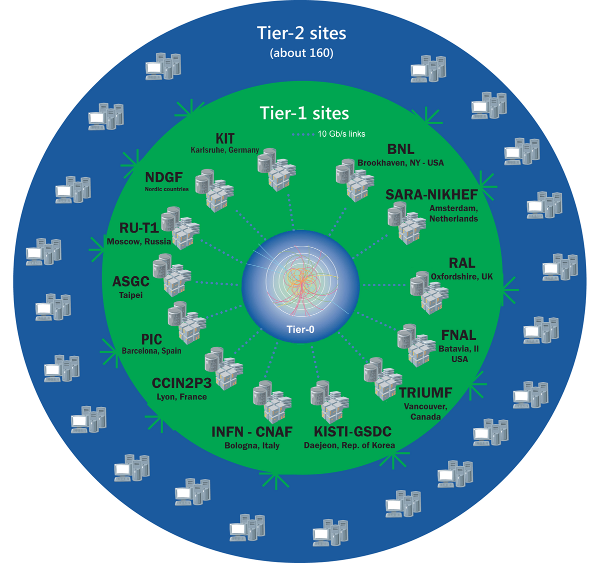
\includegraphics[width=0.5\textwidth]{img/CERNtiers}

\end{centering}

\protect\caption{CERN Tier distribution}
\end{figure}


The \ac{WLCG} is a global computing infrastructure whose mission
is to provide computing resources to store, distribute and analyze
the data generated by the \ac{LHC} seeking to be available equally
to all members, regardless of their location. A worldwide collaboration
between different experiments of the \ac{LHC} (ALICE, ATLAS, CMS
and LHCb, an scheme of them can be checked on~\ref{fig:cernexperiments})
and participating computing centers manage and organize their resources,
all coordinated by CERN~\cite{1_wlcg.web.cern.ch_2015}.

\begin{figure}
\begin{centering}\label{fig:cernexperiments}

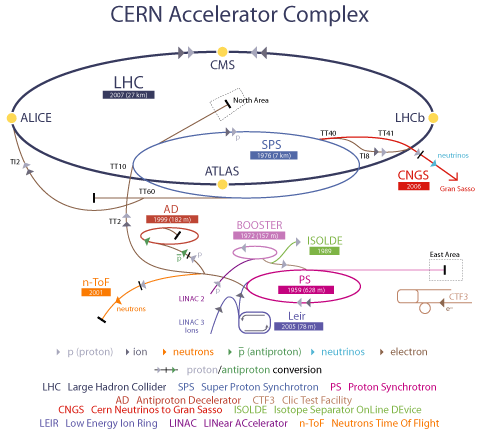
\includegraphics[width=1\textwidth]{img/CERNexperiments}

\end{centering}

\protect\caption{CERN experiments}
\end{figure}


A \ac{SE} provides uniform access to data storage resources. They
can support different data access protocols and interfaces, a \ac{SE}
may control simple disk servers, large disk arrays or tape-based \ac{MSS}. 

The \ac{SRM} is a middleware component whose function is to provide
dynamic space allocation and file management on shared storage components
on the grid. More precisely, the SRM is a grid service with several
different implementations and varying capabilities~\cite{SRM_2013_6829}.

The storage components used in the grid belong to the category of
software systems whose goal is to cluster storage resources and make
them available to data processing clients as if they were a unique
system. These products work by managing and distributing data across
mountpoints that are spread through many servers. Clients that want
to access the repository are redirected to the best machine according
to various criteria, typically given by some clustering algorithm.
There are different clustering techniques using various technologies
and the goal of such systems is always to hide to the users the complexity
linked to the “where is my file problem”. The central systems that
schedule analysis jobs to be submitted, or the users themselves do
not need to deal with details that are internal to the site (e.g.
the names of the mount points, which can change); they need to interact
with a coherent storage service that is offered and administered by
the site~\cite{1742-6596-513-3-032034}.

Some of the different solutions employed in the WLCG are:
\begin{itemize}
\item BestMAN: Disk or \ac{MSS} based storage server. 
\item CASTOR: Tape storage with disk buffer and large-scale \ac{MSS}.
\item dCache: An access point, multiple nodes. \ac{MSS} and large-scale
disk array storage systems
\item EOS: Follows the idea of a model transition from a hierarchical storage
system to a tier model.
\item StoRM: Takes advantage of the underlying file-systems to implement
the features offered by the SRM interface.
\item DPM (Disk Pool Manager): Disk-based, maximum 10TB per node. 
\end{itemize}

\section{Motivation\label{sec:Motivation}}


\subsection{Disk Pool Manager}

After this small presentation about CERN, we are in position to talk
about Disk Pool Manager. DPM is a lightweight storage solution for
grid sites, focusing on disk-based systems. It offers a simple way
to create an storage node on the network and offers compatibility
with relevant protocols (SRM, gridFTP, RFIO), for both file management
and access. It is focused on smaller sites (including simple installation
and configuration as well as easy maintenance), but also provides
all the needed functionality for a storage system on network/grid
(support for multiple server nodes, different namespaces or multiple
replicas in disk pools)~\cite{2_manzi_2015}. It is currently installed
in 165 different sites, with more than 190 instances running as of
September 2015, you can check this in figure~\ref{fig:currentusage}
and in~\cite{WLCG_stats}. 

\begin{figure}
\begin{centering}\label{fig:currentusage}

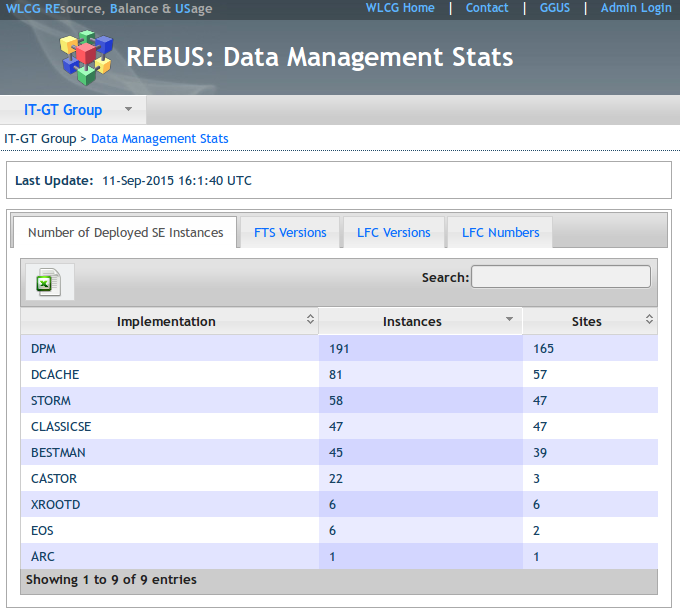
\includegraphics[width=1\textwidth]{img/DPMuse}

\end{centering}

\protect\caption{DPM current usage}
\end{figure}


Some of the most important supported features are: 
\begin{itemize}
\item Provide HTTP multi-stream transfers for high performance wide area
networks.
\item Support for third party copies. 
\item Support for X.509 authentication with proxy certificates and \ac{VOMS}
extensions 
\item Support for user credential delegations. 
\item Support for modern configuration and monitoring solutions based on
the industry standards Puppet and Nagios.
\end{itemize}

\subsection{Current goals}

The WLCG data transfer services have been one of the keys to the success
of the management of the huge volumes of LHC data, and bringing those
services and underlying infrastructure up to scale was the subject
of many of the large scale data challenges prior to the LHC switch
on. In recent years, the overall goal has been to leverage standards
and standard practices, and use them to contribute the components
that are needed to fulfill the complex problem of data access in High
Energy Physics while using technologies and toolsets that are attractive
also for non-\ac{HEP} communities, making long term sustainability
a closer goal. 

This is happening because, so far, all the bulk data movement has
relied on the gridFTP protocol. While it has been proven successful,
this protocol relies on dedicated software that must be maintained
by the \ac{HEP} grid community. This was needed in the first years,
but nowadays, in the Big Data era, there are many examples of large
scale data movement using more common protocols such as HTTP. This
change includes the advantage that there are many known solutions
to store and manage data using HTTP (including web caches, redirection
for load balancing or fail-over, etc.), that would not need dedicated
(or standalone) support from the \ac{HEP} community~\cite{1742-6596-396-3-032042}.

One of the IT-SDC-ID section contributions to the usage of HTTP in
High Energy Physics has been the evolution of the Disk Pool Manager
(DPM) architecture towards a scalable and flexible framework for designing
data management systems, called dmlite. There has been work invested
in implementing HTTP as an alternative to gridFTP. Therefore, a few
years ago, moving towards the adoption of standards to facilitate
its use and trying to eliminate the need for special tools, a WebDAV
interface (an extensión of the HTTP protocol) was implemented in Disk
Pool Manager~\cite{1742-6596-396-5-052006}. The main goal was to
facilitate the access to the storage network through common programs,
i.e. web browsers or WebDAV clients. 

However, this implementation is based on a primitive read-only interface
when accessed through a web browser, which limits the use cases to
simple directory browsing and file downloads. This makes still necessary
to use special tools for certain operations such as file uploads. 


\section{Objectives and scope\label{sec:Objectives-and-scope}}

Taking advantage of this WebDAV interface, the general goal of DPMbox
project is to offer a truly friendly interface that concentrates all
possible functionality in one tool that can be used with programs
known by users, namely web browsers. The purpose is not to create
a cloud storage system copycat, but to get advantage of the features
that DPM system already offers (performance, different accessing protocols,
data replication, etc.) adding the ease of use of the increasingly
widespread cloud storage systems like Dropbox, OneDrive or Google
Drive.

More specifically the system must allow users to browse and access
their data stored in DPM grid elements that provide the HTTP protocol
in a manner that is straight forward for unexperienced users. The
focus will be held mainly on usability and ease of use but other requirements
must also be taken into consideration, including, obviously, security
constraints. 

The development will focus on the functionality required by the IT-SDC-ID
section, pursuing effectiveness on DPM infrastructure. But one of
the future goals is that, after fulfilling these requirements, DPMbox
can be adapted easily to another contexts, enabling its general use
with any other system implementing a WebDAV protocol.

As a web development the project will use standard web technologies
as HTML5~\cite{2_w3.org_2015}, CSS3~\cite{3_w3.org_2015} or JavaScript~\cite{4_mozilla_developer_network_2015}
and like all software involved in DPM, the project will be developed
under the Apache License version 2.0~\cite{5_apache.org_2015}.


\section{Glossary}


\subsection{Acronyms}

\begin{acronym}
  \acro{AC}{Attribute Cetificate}
  \acro{ACL}{Access Control Lists}
  \acro{CERN}{European Organization for Nuclear Research}
  \acro{DAV}{Distributed Authoring and Versioning}
  \acro{DN}{Distinguished Name}
  \acro{DPM}{Disk Pool Manager}
  \acro{EGI}{European Grid Infrastructure}
  \acro{FQAN}{Fully Qualified Attribute Name}
  \acro{HEP}{High Energy Physics}
  \acro{LFC}{LCG File Catalog}
  \acro{LFN}{Logical File Name}
  \acro{LHC}{Large Hadron Collider}
  \acro{MSS}{Mass Storage System}
  \acro{PFN}{Physical File Name}
  \acro{PMI}{Privilege Management Infrastructure}
  \acro{RFIO}{Remote File Input Output}
  \acro{SE}{Storage Element}
  \acro{SFN}{Storage File Name}
  \acro{SRM}{Storage Resource Manager}
  \acro{TFG}{Trabajo Fin de Grado - Degree Thesis}
  \acro{UCA}{Universidad de Cádiz}
  \acro{UX}{User eXperience}
  \acro{VOMS}{Virtual Organization Membership Service}
  \acro{WLCG}{Worldwide LHC Computing Grid}
  \acro{XHR}{XMLHttpRequest}
  \acro{XML}{eXtended Markup Language}
\end{acronym}


\subsection{Definitions}
\begin{description}
\item [{Collection}] A collection is defined as a resource whose state
consists of at least a list of internal member URIs and a set of properties,
but which may have additional state such as entity bodies returned
by GET. In this work you can almost consider as a synonym to a directory.
Complete and formal definition can be found on section 5.2 of RFC
4918~\cite{RFC4918}.
\item [{Metalink}] Metalink is an extensible metadata file format that
describes one or more computer files available for download. It specifies
files appropriate for the user's language and operating system, facilitates
file verification and recovery from data corruption, and lists alternate
download sources (mirror URIs)~\cite{RFC5854,RFC6249}.
\item [{POSIX}] Acronym for Portable Operating System Interface, a family
of standards specified by the IEEE Computer Society for maintaining
compatibility between operating systems. POSIX defines the application
programming interface (API), along with command line shells and utility
interfaces, for software compatibility with variants of Unix and other
operating systems.
\item [{Proxy~Certificate}] The term Proxy Certificate is used to describe
a certificate that is derived from, and signed by, a normal X.509
Public Key End Entity Certificate or by another Proxy Certificate
for the purpose of providing restricted proxying and delegation within
a PKI (Public Key Infrastructure) based authentication system~\cite{rfc3820}.
\item [{X.509}] An ITU-T (Telecommunication Standardization Sector) standard
for a PKI (Public Key Infrastructure) and PMI (Privilege Management
Infrastructure). X.509 specifies, amongst other things, standard formats
for public key certificates, certificate revocation lists, attribute
certificates, and a certification path validation algorithm~\cite{rfc3820}.
\end{description}

\section{Document organization\label{sec:Document-organization}}

In this \emph{Introduction} you can read about the project motivation
and some descriptions about how the CERN works, giving some context
to the project. This is naturally followed by the \emph{State of the Art},
so the reader can completely envision the current system and environment
state. 

After that comes the \emph{Schedule}, all the organization and planning
stuff can be found there. 

Then, in the \emph{Project general description} you can read about
what has been developed in a non-technical way, before getting into
detail in the next section, \emph{Project development}, where all
things about how DPMbox has been built are shown: system analysis,
design, implementation and testing.

Next come \emph{Conclusions} and \emph{Acknowledgements}, where
we explain the final thoughts that have been reached after completing
the development.

Finally, an appendix is presented, where different manuals can be
found (\emph{Installation}, \emph{Development} and \emph{User}),
and also the \emph{License} under which this document is published.


\chapter{State of the art\label{chap:State-of-the}}

As said before, right now there is already web access implemented
in the Disk Pool Manager infrastructure. This has been developed as
part of the HTTP/WebDAV front-end and is built getting advantage of
the Apache WebDAV module, \code{mod\_dav}, and the proxy support
module, \code{mod\_gridsite}. To get a deeper understanding of how
it works a paper from his authors, Álvarez Ayllón et al., can be checked~\cite{1742-6596-396-5-052006}.

The Hypertext Transfer Protocol (HTTP)\textsuperscript{}is a well
known and widely implemented standard protocol based on a client-server
stateless model. It can be used as a data transfer protocol, where
users request a resource to a specific server, which then sends the
response back. 

Web Distributed Authoring and Versioning (WebDAV) is an extension
to the HTTP protocol that provides namespaces and metadata handling
through the web. 
\begin{description}
\item [{Namespace}] Users can create, rename, modify and remove elements
trough the web.
\item [{Metadata}] Users can create and retrieve resources, and also modify
its associated properties, as owner, description, permissions and
any other information that can be expressed as text or XML. 
\end{description}


For this goal it defines some new additional methods to the traditional
ones (POST, GET, PUT) like PROPFIND, MKCOL… It uses XML to encode
the answers, as the list of properties of a file, or the content of
a folder. Complete specification can be read in~\cite{RFC4918}. 

In the current web visualization you can explore a collection, download
the data and navigate through a collection. But is not possible to
upload data, there is no interaction. A reason for this is that HTML
forms don’t support more HTTP verbs/methods than just GET and POST,
and no PUT. So until now for this cases the use of CURL or a proper
WebDAV client is needed. The current view accessing a DPM server through
a web browser is depicted in~\ref{fig:webdavaccess}.

\begin{figure}
\begin{centering}

\label{fig:webdavaccess}

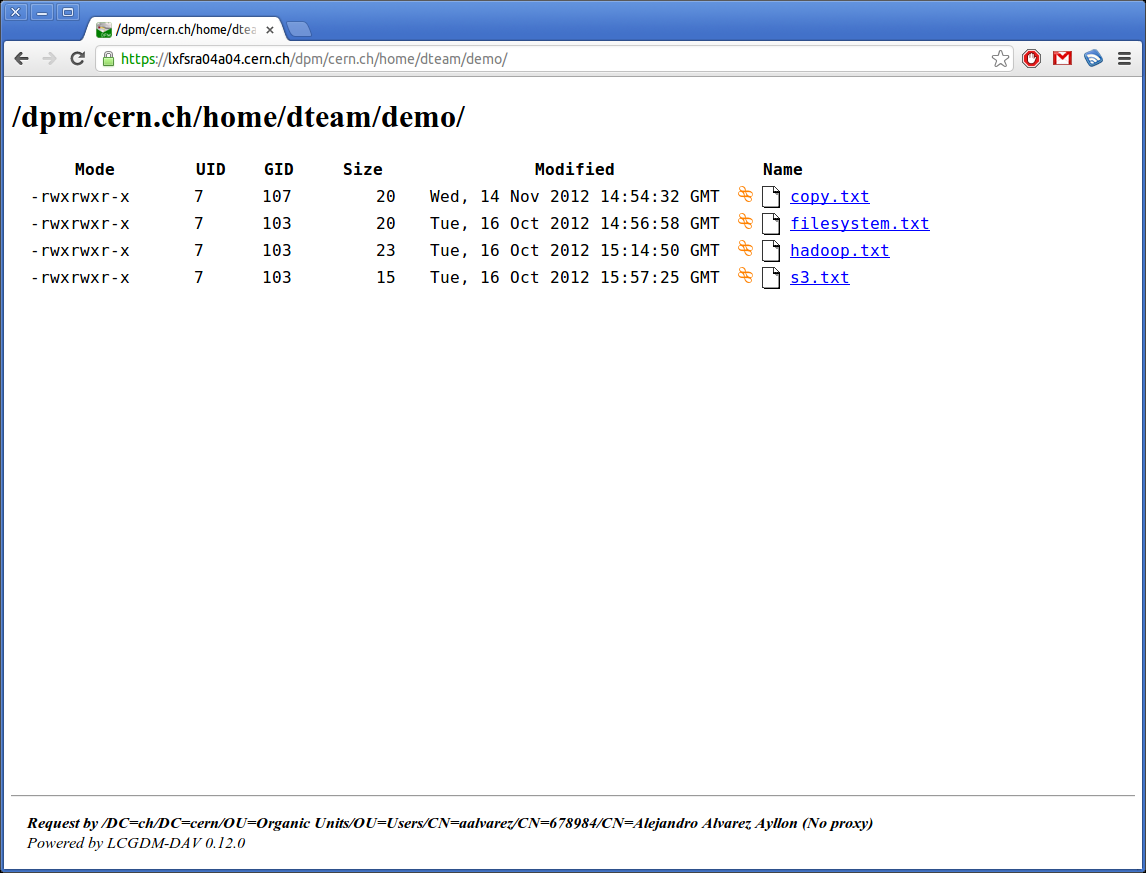
\includegraphics[width=1\textwidth]{img/DPM_currentaccess_1}

\end{centering}

\protect\caption{WebDAV access view}
\end{figure}



\section{DPM and LFC}

The \ac{DPM} and \ac{LFC} are two grid components with more than
240 endpoints available. 

The purpose of the \ac{LFC} is to allow the access and retrieval
of any file using just its \ac{LFN}, without the need of knowing
where exactly it is replicated. When a user does a request to an \ac{LFC},
it will return a list of \ac{SFN} where this file can be retrieved. 

\ac{DPM}is a lightweight storage system mostly targeted at Tier-2
and medium size sites, providing reliable and scalable storage while
keeping configuration and management simple. It maps a \ac{SFN} to
a Transfer URL (TURL), which is the association between a Physical
File Name (\ac{PFN}) and an access protocol such as \ac{RFIO}, HTTP
or gridFTP.


\section{Access}

Currently, when a user wants to retrieve a file, a catalog must be
queried for different replicas of that file. Then, the client will
be redirected to the site hosting that replica, and finally to its
actual physical location within that site. Generally this is done
automatically, but specific tools are needed. 

HTTP supports this kind of behavior as the response of a request can
be a redirection to a different location than the one originally demanded.
The functionality is the same, but as it is an extremely wide implemented
standard, data could be accessed from almost any kind of platform,
from servers to mobile devices. 

WebDAV give in addition, metadata handling. It is also a popular protocol,
with clients available for a wide variety of operating systems. 

With support to these standards users are allowed to access their
data easily and transparently, from any machine, through any platform,
and using clients they already know how to use, for instance, web
browsers. 


\subsection{HTTP clients}

A DAV server can be accessed safely using plain HTTP, which allows
using regular web browsers (Mozilla Firefox, Google Chrome, Opera...)
to explore a DAV endpoint an retrieve files. However, web browsers
don’t usually allow uploading files directly - without using a web
form - so for that purpose CURL can be used. CURL is a command line
interface able to interact with several protocols, being HTTP one
of them. We compare the support of some key features of two of the
most frequent tools used to access a web server in table \ref{tab:http_clients}. 

\begin{table}[h]
\label{tab:http_clients}

\begin{tabular}{cccccccc}
\textbf{Client} & \textbf{OS} & \textbf{GUI} & \textbf{CLI} & \textbf{X.509} & \textbf{X.509 proxies} & \textbf{Redirections} & \textbf{PUT}\tabularnewline
\hline 
CURL & Any & No & Yes & Yes & Yes & Yes & Yes\tabularnewline
Web browser & Any & Yes & No & Yes & Only IE & Yes & No\tabularnewline[\doublerulesep]
\end{tabular}
\begin{description}
\item [{OS}] Operating System 
\item [{GUI}] Graphical User Interface 
\item [{CLI}] Command Line Interface
\item [{X.509}] Support for client certificates
\item [{X.509~proxies}] Support for proxy certificates 
\item [{Redirections}] Follows redirections when needed
\item [{PUT}] Writing support 
\end{description}
\protect\caption{HTTP clients}
\end{table}



\subsection{WebDAV clients}

Yo perform namespace operations, such as creating directories, renaming
or fetching properties, WebDAV must be used. We present a comparison
between the most popular WebDAV clients on~\ref{tab:webdav_clients}. 

\begin{table}
\label{tab:webdav_clients}

\begin{tabular}{ccccccc}
\textbf{Client} & \textbf{OS} & \textbf{GUI} & \textbf{CLI} & \textbf{X.509} & \textbf{X.509 Proxies} & \textbf{Redirections}\tabularnewline
\hline 
Cadaver & {*}nix & No & Yes & Yes & No & No\tabularnewline
Davlib & OS X & Yes & No & No & No & Yes\tabularnewline[\doublerulesep]
Shared folder & Windows & Yes & Yes & Yes & Yes & Not on Win7\tabularnewline[\doublerulesep]
DavFS2 & {*}nix & N/A & Yes & Yes & No & No\tabularnewline[\doublerulesep]
gvfs ≥ 1.12.1 & Gnome 3 & Yes & No & No & No & Not on PUT\tabularnewline[\doublerulesep]
Dolphin & KDE & Yes & No & No & No & Yes\tabularnewline[\doublerulesep]
Cyberduck & Win, OS X & Yes & No & No & No & Yes\textsuperscript{1}\tabularnewline[\doublerulesep]
libneon & {*}nix & N/A & N/A & Yes & No & No\tabularnewline[\doublerulesep]
\end{tabular}

\bigskip

\bigskip

\bigskip

\emph{\textsuperscript{(1)} Added support for PUT redirections on version
4.4.4~\cite{1_trac.cyberduck.io_2015}}

\protect\caption{WebDAV clients}
\end{table}



\section{Security\label{sec:Security} }

In terms of authentication information for authorization, grids use
X.509 \ac{AC}s and \ac{PMI}s~\cite{wiki:PMI} to assign privileges
to users, and to carry the privileges around the Grid. \ac{DPM} uses
X.509 and a grid privilege management system called \ac{VOMS}. 

In a nutshell, \ac{VOMS} provides the tools to enable Virtual Organizations
and attribute-based authorization in distributed contexts. \ac{VOMS}
supports a rich registration process compliant with the \ac{EGI}policies
on VO registration services. Users can be organized in groups and
can be assigned roles and other types of attributes. User privileges,
in the shape of VO memberships and roles, are placed inside an X.509
\ac{AC} by the \ac{VOMS} server, signed by the \ac{VOMS} server,
and then embedded in the user's X.509 proxy certificate for carrying
around the grid~\cite{AlfieriCCdFGLS03}.

Once the clients are authenticated, the X.509 certificate \ac{DN}
is used as a \code{\_user name\_} and the \ac{VOMS} \ac{FQAN} are
used as \code{\_group names\_}. Apart from this, DPM authorization
follows the POSIX filesystem authorization semantics, and it supports
(and, indeed, requires) \ac{ACL} on its namespace..


\chapter{Schedule\label{chap:Schedule}}

In this section we cover the schedule the project has followed. Specifically
we talk about the the personnel involved, the chosen development methodology,
the stages the project has gone through and its planning.


\section{Life cycle model}

The ISO/IEC 12207-1~\cite{ISO12207} standard defines the life cycle
model as a 
\begin{quote}
“\emph{framework of processes and activities concerned with the life cycle
that may be organized into stages, which also acts as a common reference
for communication and understanding}”
\end{quote}


The chosen development methodology for DPMbox was the iterative and
incremental model, an structured and agile software development methodology. 

The life cycle is summarized in a set of iterations. The phases of
the life cycle are analysis, design, implementation, testing, operation
and maintenance. After performing the analysis (getting requirements
specification) and application design (defining the system's architecture),
we start to code already, obtaining a very limited initial release.
This version will be tested and in case of positive results, we go
back to the implementation phase where this initial version will be
expanded, adding new features or improving the existing ones. This
step has to be repeated as many times as necessary until the expected
final version has been reached, when the project moves to the exploitation
phase. If the tests don't give the expected results, we must return
to the analysis stage to find out the problems relating to this version
and redirect it. Finally, during exploitation phase, errors or mandatory
improvements could be expected. Then it will be time to move on to
the maintenance phase, where these incidents will be addressed before
moving back to the analysis phase. 

After summarizing this process, we can say that our model is incremental
and iterative, thereby we have created product versions that have
slowly grown in features and performance until a final product stage
has been reached. 


\section{Stages}

Here you can read a small brief about the features that particularize
each of the stages that DPMbox has gone through. CERN network access
has been granted for a year, so the development must be adjusted to
that access to allow the needs of on-site deployment, information
obtainment... You can get the big picture at a glance having a look
at the Gantt chart, figure~\vref{fig:gantt}.


\subsection{First stage, first approach}
\begin{itemize}
\item Get familiar with the CERN network, the IT-SDC-ID section and all
the terminology of its systems.
\item Disk Pool Manager investigate and learn about through its documentation.
\item Study different approaches and decide which one is the better option.
\item Master the concepts, verbs and particularities of the WebDAV protocol,
as it looks as the easiest way to approach DPM. 
\item Get everything ready for the first CERN visit, trying to assure to
make the most of the time I'll be there.
\end{itemize}

\subsection{Second stage, connection library}
\begin{itemize}
\item Deep learning about JavaScript, since a development based on this
language was chosen.
\item Study AJAX calls, the way of communicating with the WebDAV gateway.
\item Start to develop a WebDAV connection library. This follows a minimal
viable product approach, starting with a simple call just to read
the information about a WebDAV server, then read its contents then...
\item Prepare for the Naples DPM workshop. I was invited to contribute to
this annual DPM group meeting with a small presentation about DPMbox. 
\item Build of first working prototype.
\end{itemize}

\subsection{Third stage, user interface}
\begin{itemize}
\item Begin an intensive \ac{UX} learning.
\item Decide the final design between some different approaches.
\item Investigate w2ui, test it a lot. A jQuery UI based interface and other
possibilities were discarded.
\item Transform the sketch prototype into the actual interface.
\end{itemize}

\subsection{Fourth stage, integration}
\begin{itemize}
\item Extending the interface and the WebDAV connection library integrating
it into the Disk Pool Manager software stack.
\item Test the integration between the library and the interface.
\item Get everything ready for the second and final visit to CERN.
\item Build the second working prototype.
\end{itemize}

\subsection{Fifth stage, deployment}
\begin{itemize}
\item Complete a series of full tests. 
\item Deploy DPMbox on site.
\item Prepare the project's participation in the IX CUSL (Concurso Universitario
de Software Libre) final phase.
\item Address different issues and comments received from external feedback.
\end{itemize}
\begin{figure}
\begin{centering}

\label{fig:gantt}

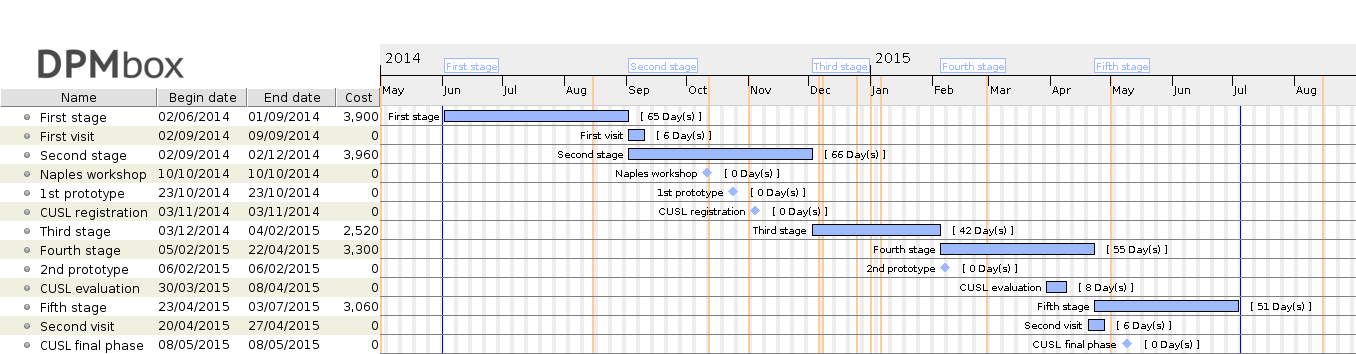
\includegraphics[angle=90,height=1\textheight]{img/GanttChart}

\end{centering}

\protect\caption{Gantt chart}
\end{figure}



\section{Organization}

The project has been developed entirely by the writer, student of
\emph{Universidad de Cadiz}, carrying out the work of analysis, design
and development, including also visual interface design. The project
development has been reviewed and guided by supervisors Alejandro
Álvarez Ayllón, current employee at CERN IT-SDC-ID section, and Manuel
Palomo Duarte, PhD Computer Science in \emph{Universidad de Cádiz}.


\section{Non-Human resources\label{sec:Non-Human-resources}}

As a free software project, DPMbox has been developed using a lot
of open source and free technologies: Git, jQuery, w2ui... You can
read more about the libraries and tools employed in the sections~\ref{sub:Version-control},~\ref{sub:Program-languages-and}
and~\prettyref{sub:Tools}. What is important to bring out in this
section is that these tools are not only free, as in speech, but also
free as in beer.

For the ordinary development, we have used a laptop with an Apache
local server, activating its WebDAV modules. In the hardware section
we have:
\begin{itemize}
\item HP Pavilion DV6 3040ES with the following technical specification:

\begin{itemize}
\item Intel Core i7 Q720 Processor
\item 4GB Memory
\item 128GB SSD Crucial M4
\item GNU/Linux Ubuntu 10.04 and GNU/Linux Mint 17 as OS
\end{itemize}
\end{itemize}


Then, to have some testing outside the local scope from time to time
an external cloud server has been hired:
\begin{itemize}
\item Digital Ocean SSD droplet with these characteristics:

\begin{itemize}
\item 1 Core Processor 
\item 512MB Memory 
\item 20GB SSD Disk 
\item 1TB Transfer 
\item GNU/Linux Ubuntu 14.04 32bits
\end{itemize}
\end{itemize}


Also, in different development stages DPMbox prototypes have been
deployed in DPM testing instances in CERN IT-SDC-ID section servers.
The configuration of these machines could be varied, with most of
them using Scientific Linux 6 as it OS.


\section{Costs}

Project total cost (C) is the aggregate of the material and human
resources cost.

\begin{centering}\bigskip

$TotalCost(C)=MaterialCost(C_{m})+PersonnelCost(C_{p})$

\end{centering}\bigskip

Material costs (C\textsubscript{m}) are constituted by the cost of
software (C\textsubscript{s}) and hardware (C\textsubscript{h}).

As seen on previous section the infrastructure requirements for the
development have been humble, basically the project has only need
a single PC computer with GNU/Linux and internet connection (about
400€ for a 10 month long contract). The tools and libraries used were
all free to use in this context, therefore neither requires cost.
The price of the personal computer used in the development was 790
€. Also the monthly rate of the Digital Ocean server is \$5 (though
this was really hired through GitHub Education developer pack~\cite{github_education_2015}).
The €/\$ exchange rate as of September 1st 2015 makes that 4.4€, so
the use of a Digital Ocean droplet for ten months will cost 44€.

\begin{centering}\bigskip

\[
MaterialCost(C_{m})=SoftwareCost(C_{s})+HardwareCost(C_{h})=0+400+790+44=1,234.8\lyxmathsym{€}
\]


\end{centering}\bigskip

In terms of time, the completion of this project required 1,395 hours
of work or 8.72 persons per month. In the Gantt chart it can be seen
that the project is planned to be finished in 279 days (each of the
five stages lifespan), but the project has matched in time with a
part-time job, so the amount of time dedicated to the project has
been 5 hours per day.

To calculate the staff wage we are taking three different documents:~\cite{salaries1_BOCM,salaries2_MichaelPage,salaries3_UCA}
(all of them in spanish and centered on spanish job positions since
the cost of developing with CERN based salaries would be very different).
The first one gives us a 1,850.12€ monthly wage for a group 1 worker
(University degree engineers and so), second one stands that a Systems
Analyst position has an average salary of 1,875€, and in the last
one we read that a Computer Engineer has a salary of 1,353.22€ per
month. With the data from this documents we have estimated a salary
that would be: 1,692.8€

\begin{centering}\bigskip

\[
Staff\,Cost=Monthly\,wage\,\text{×}\,Persons\,per\,month=1,692.8\times8.72=14,761,22\lyxmathsym{€}
\]


\end{centering}\bigskip

Also, the CERN visits have had a cost of 900€ each (including travels,
accommodation and subsistence allowance).

\begin{centering}\bigskip

\[
Personnel\,Cost(C_{p})=Staff\,Cost+Additional\,Cost=14,761.22+900+900=16,561.22\lyxmathsym{€}
\]


\end{centering}\bigskip

And with all this data we can now calculate the total costs of the
project:

\begin{centering}\bigskip

\[
C=C_{m}+C_{p}=1,234.8+16,561.22=17,796,02\lyxmathsym{€}
\]


\end{centering}\bigskip


\section{Risks}

A risk is defined as an uncertain event which should it occur, will
have an effect on the project meeting its objectives. The risk management
purpose is to reduce the probability and impact of threats, identifying,
studying and eliminating sources of risk before they threaten the
project's success. Based on this, we list a number of risks that may
affect DPMbox and should be addressed:
\begin{itemize}
\item The development team hasn't been able to meet or know directly the
needs of any final user. The aim is to develop a generalized software,
based on our assumptions as developers. There is a risk that the system
is not accepted in general terms by potential users.

\begin{itemize}
\item Impact: All phases could be affected, because the problem lie in the
of requirements definition. Therefore, all development on the basis
of these requirements may be in vain.
\item Probability: The probability of occurrence will depend on the needs
of the public to be targeted and the quality and reliability of software
obtained.
\item Priority: Avoiding this risk is a top priority, as it could mean having
worked for months in features not needed, or viceversa. 
\item Action~plan: To prevent this from happening, some working prototypes
are planned. They can be shown to some acquainted DPM users, that
way we can know their point of view.
\end{itemize}
\item Late delivery due to lack of knowledge about tools, languages, or
even more likely the ​​DPM system characteristics.

\begin{itemize}
\item Impact: This risk can affect all phases, because in all of them the
developer requires the use of the tools and a knowledge on the system.
\item Probability: The probability of occurrence is high since the developer
does not have any previous experience with the system.
\item Priority: The priority will be lower as the project progresses, the
learning curve is expected to be steep.
\item Action~plan: It would be ideal to know the different tools and having
ever used such a system like DPM, but this time is not possible to
avoid the risk. However, we will try to do a good learning process
for each tool, language, and also the system.
\end{itemize}
\end{itemize}

\chapter{Project general description\label{chap:Project-general-description}}

\begin{figure}[H]
\begin{centering}\label{fig:logo}


\includegraphics[width=0.25\textwidth]{DPMbox}

\end{centering}

\protect\caption{DPMbox logo}
\end{figure}



\section{Product outlook}

The Disk Pool Manager (DPM) is a lightweight grid storage component,
allowing access to data using commonly used grid protocols over the
\ac{WLCG}. The developed project, DPMbox, is its new web-based interface
developed in JavaScript. 

Its look and feel is similar to desktop file explorers, so a new user
won’t spend lots of time to adapt to its behaviour. In terms of it
functionality, it's possible to perform various operations, including
(multiple) file upload, (multiple) file download, (multiple) delete
of files and collections. Besides that you can also perform searches
based on various file properties inside a directory and sort the content
by those same properties. Its panels are slightly responsive for a
fast adjustment to your screen, and besides that, it has a flexible
layout, that you can adapt to suit your needs.

It has a very small size, 79KB (not including external libraries).
With all its libraries included (jQuery, w2ui) the load size could
be less than 200KB (all files minified).

The main purpose of DPMbox is to support the Disk Pool Manager system,
however, it follows the standard WebDAV RFC 4918~\cite{RFC4918}
aiming to be compatible with any WebDAV server. It has has been developed
modularly, and its internal library could be used to develop other
new applications.

Chrome/Chromium, FireFox 7+, Safari 5+ and IE 9+ are among supported
browsers.

\begin{figure}[H]
\begin{centering}\label{fig:fed_screenshot}

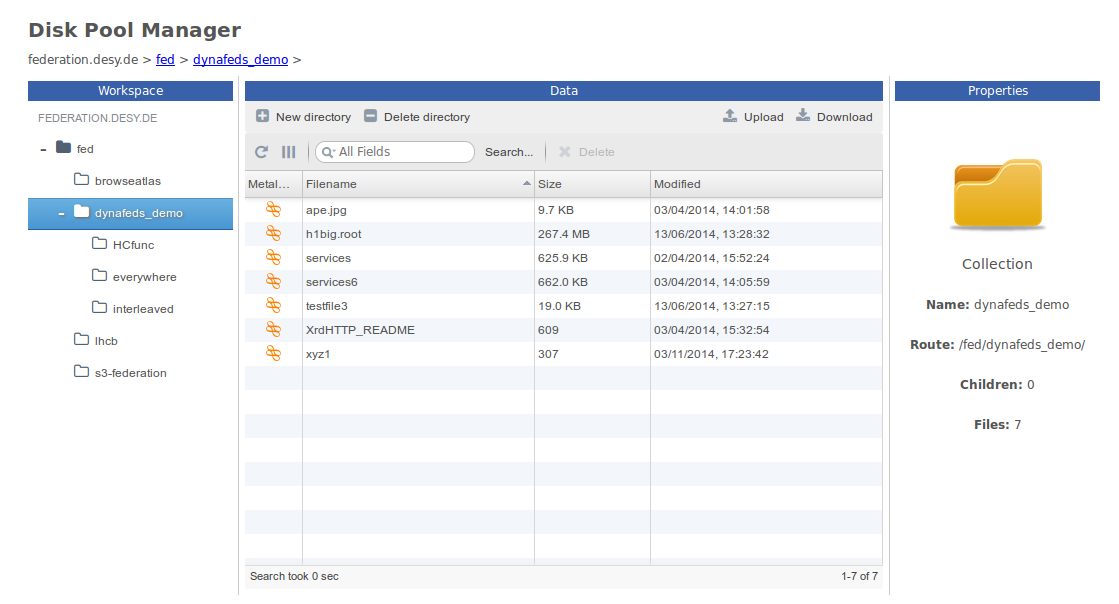
\includegraphics[width=0.5\textwidth]{img/FedScreenshot}

\end{centering}

\protect\caption{DPMbox in action}
\end{figure}



\section{Repositories}

DPMbox interface is integrated into version 0.16 of \code{lcgdm-dav}
package. After going through various testing stages is already, as
of September 2015, available to download and install from repositories
for Fedora 22 and Fedora 23. It's still on testing repositories for
EL-5, EL-6 and EL-7. By the way, EPEL (Extra Packages for Enterprise
Linux) is a volunteer-based community effort from the Fedora project
to create a repository of high-quality add-on packages that complement
the Fedora-based Red Hat Enterprise Linux (RHEL) and its compatible
spinoffs, such as CentOS and Scientific Linux.

The l\code{cgdm-dav} package status on the repositories can be checked
on~\ref{fig:lcgdm-dav_status}.

\begin{figure}[H]
\begin{centering}

\label{fig:lcgdm-dav_status}

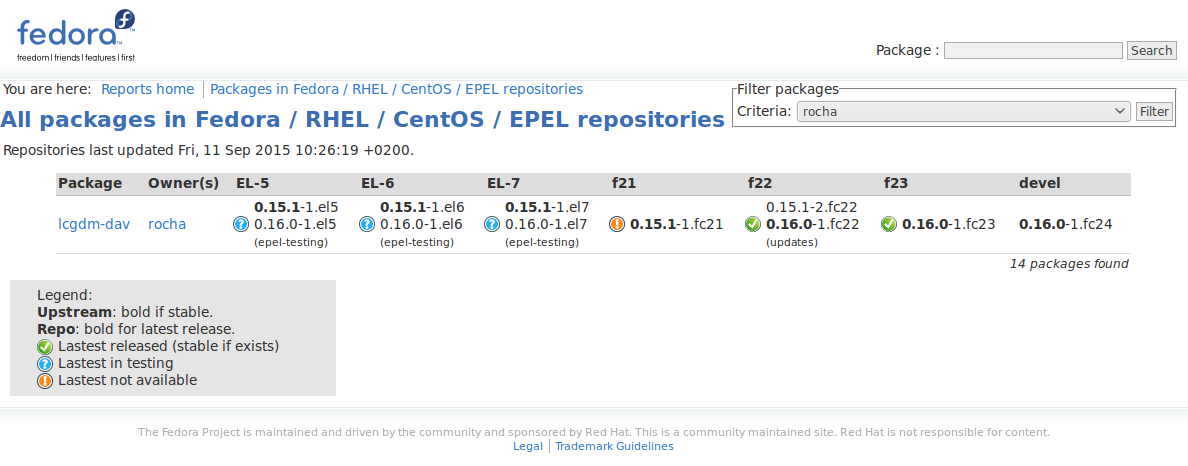
\includegraphics[width=1\textwidth]{img/lcgdm-dav_status}

\end{centering}

\protect\caption{lcgdm-dav package status}
\end{figure}



\section{User characteristics}

The vast majority of \ac{WLCG} users are members of \ac{LHC} experiments
or affiliated research projects and should normally use the official
software frameworks that are available per experiment or project.
Those frameworks in turn make use of more generic middleware components,
which are different in the different infrastructures that make up
WLCG: EGI (European Grid Infrastructure), NDGF (Nordic Data Grid Facility),
OSG (Open Science Grid) and other partners. For service administrators
and operations managers each participating infrastructure has documentation
on how to use or test services. 

Currently, the majority of users of the \ac{WLCG} come from the \ac{HEP}
community for which the \ac{WLCG} is a necessity to analyze the data
generated by the \ac{LHC} experiment at CERN in Geneva. However,
a growing number of \ac{WLCG} users come from many other scientific
disciplines, such as the biomedical field, earth science, astrophysics,
fusion science, etc.

Generally speaking, we can consider our target user a not necessarily
high level at technical user, but acquainted at file browser interfaces
or even cloud storing services. And anyway, as you can see, the potential
DPMbox user profile, being mostly science researchers, could be quite
heterogeneous. Furthermore one of the objectives is to attract new
users to this interface, particularly the non-\ac{HEP} users, so,
audacious it may sound, we are aiming to design a, universally appealing
interface, or at least the design won't be focused on a specific niche
audience. 


\chapter{Project development\label{chap:Project-development}}

In this chapter are described all the details related with how DPMbox
has been constructed: objectives, requirements, solution alternatives,
system analysis, design, implementation and testing.


\section{System objectives\label{sec:System-objectives}}

The main objectives of DPMbox, from a general point of view, are listed
below. These objectives summarize in a very roughly way the functionality
of the project:

\begin{table}[h]
\begin{tabular}{|>{\centering}p{0.15\textwidth}|>{\raggedright}p{0.8\textwidth}|}
\hline 
 & Create an integrated application\tabularnewline
\hline 
Description & DPMbox must be a piece of software that can be integrated with the
rest of Disk Pool Manager software stack.\tabularnewline
\hline 
\end{tabular}

\protect\caption{OBJ-1}
\end{table}


\begin{table}[h]
\begin{tabular}{|>{\centering}p{0.15\textwidth}|>{\raggedright}p{0.8\textwidth}|}
\hline 
 & Develop a usable interface\tabularnewline
\hline 
Description & The interface developed for DPMbox must be user appealing, being easy
to familiarize and fast to master, following standard recommendations
in terms of usability and accessibility.\tabularnewline
\hline 
\end{tabular}

\protect\caption{OBJ-2}
\end{table}


\begin{table}[h]
\begin{tabular}{|>{\centering}p{0.15\textwidth}|>{\raggedright}p{0.8\textwidth}|}
\hline 
 & Connect and interact with a WebDAV server\tabularnewline
\hline 
Description & The system must be able to access a WebDAV server, being able to read
and understand its information and commands, interacting with it in
a way the communication can flow both ways.\tabularnewline
\hline 
\end{tabular}

\protect\caption{OBJ-3}
\end{table}



\section{Requirements}

A requirement is a capability that a software product must possess
or something a product must do in order to ultimately satisfy a user
need. Requirements form the basis for any software development project,
as they drive all activities that follow. As a result, it is very
important to get requirements right, otherwise, the entire project
can fail. In fact, poor requirements are among the top reasons for
project failures.


\subsection{Functional}

The functional requirements define the functions of the software system
and its components.


\subsubsection{Files}

\begin{table}[H]
\begin{tabular}{|>{\centering}p{0.15\textwidth}|>{\raggedright}p{0.8\textwidth}|}
\hline 
 & Upload a file\tabularnewline
\hline 
Description & DPMbox must be able to upload a file to the system, either through
a web form or in a drag and drop fashion. \tabularnewline
\hline 
\end{tabular}

\protect\caption{FRQ-1}
\end{table}


\begin{table}[H]
\begin{tabular}{|>{\centering}p{0.15\textwidth}|>{\raggedright}p{0.8\textwidth}|}
\hline 
 & Download a file\tabularnewline
\hline 
Description & The system must be able to download files from the server and the
user must be able to save it on its local filesystem.\tabularnewline
\hline 
\end{tabular}\protect\caption{FRQ-2}
\end{table}


\begin{table}[H]
\begin{tabular}{|>{\centering}p{0.15\textwidth}|>{\raggedright}p{0.8\textwidth}|}
\hline 
 & Delete a file\tabularnewline
\hline 
Description & The interface must offer the possibility to remove a specific file
from the server.\tabularnewline
\hline 
\end{tabular}

\protect\caption{FRQ-3}
\end{table}



\subsubsection{Directories}

\begin{table}[H]
\begin{tabular}{|>{\centering}p{0.15\textwidth}|>{\raggedright}p{0.8\textwidth}|}
\hline 
 & Create a directory\tabularnewline
\hline 
Description & It must be possible to create a directory, giving a valid name.\tabularnewline
\hline 
\end{tabular}

\protect\caption{FRQ-4}
\end{table}


\begin{table}[H]
\begin{tabular}{|>{\centering}p{0.15\textwidth}|>{\raggedright}p{0.8\textwidth}|}
\hline 
 & Read a directory\tabularnewline
\hline 
Description & It should be possible to select a certain folder and read its content,
of files and collections.\tabularnewline
\hline 
\end{tabular}

\protect\caption{FRQ-5}
\end{table}


\begin{table}[H]
\begin{tabular}{|>{\centering}p{0.15\textwidth}|>{\raggedright}p{0.8\textwidth}|}
\hline 
 & Delete a directory\tabularnewline
\hline 
Description & The user should be allowed to delete a certain folder, being it empty
or not.\tabularnewline
\hline 
\end{tabular}

\protect\caption{FRQ-6}
\end{table}



\subsection{Information}

The information requirements detail data that the system uses during
the development and execution to properly perform its operations.

\begin{table}[h]
\begin{tabular}{|>{\centering}p{0.15\textwidth}|>{\raggedright}p{0.8\textwidth}|}
\hline 
 & File\tabularnewline
\hline 
Required information & \begin{itemize}
\item Filename
\item Size
\item Modification date
\item Metalink\end{itemize}
\tabularnewline
\hline 
\end{tabular}

\protect\caption{IRQ-1}
\end{table}


\begin{table}[H]
\begin{tabular}{|>{\centering}p{0.15\textwidth}|>{\raggedright}p{0.8\textwidth}|}
\hline 
 & Collection\tabularnewline
\hline 
Required information & \begin{itemize}
\item Name
\item Path
\item Children collections
\item Files contained\end{itemize}
\tabularnewline
\hline 
\end{tabular}

\protect\caption{IRQ-2}
\end{table}



\subsection{Non-functional}

Non-functional requirements specify criteria for various categories
that the software must meet to ensure a good level of quality beyond
its functions or operations.


\subsubsection{Performance}

\begin{table}[H]
\begin{tabular}{|>{\centering}p{0.15\textwidth}|>{\raggedright}p{0.8\textwidth}|}
\hline 
 & Fast loading\tabularnewline
\hline 
Description & The system must be able to load and perform operations in a reasonable
time.\tabularnewline
\hline 
\end{tabular}

\protect\caption{NRQ-1}
\end{table}



\subsubsection{Security}

\begin{table}[H]
\begin{tabular}{|>{\centering}p{0.15\textwidth}|>{\raggedright}p{0.8\textwidth}|}
\hline 
 & Protected from attacks\tabularnewline
\hline 
Description & DPMbox should react accordingly to possible attacks compromising the
system's security.\tabularnewline
\hline 
\end{tabular}

\protect\caption{NRQ-2}
\end{table}



\subsubsection{Technology}

\begin{table}[H]
\begin{tabular}{|>{\centering}p{0.15\textwidth}|>{\raggedright}p{0.8\textwidth}|}
\hline 
 & WebDAV server\tabularnewline
\hline 
Description & To connect to the DPM server, the WebDAV protocol must be used.\tabularnewline
\hline 
\end{tabular}

\protect\caption{NRQ-3}
\end{table}



\subsubsection{Maintainability}

\begin{table}[H]
\begin{tabular}{|>{\centering}p{0.15\textwidth}|>{\raggedright}p{0.8\textwidth}|}
\hline 
 & Ease to maintain\tabularnewline
\hline 
Description & The system, and specially its internal code, should be easy to read
and understand offering an easy maintenance.\tabularnewline
\hline 
\end{tabular}

\protect\caption{NRQ-4}
\end{table}



\subsubsection{Extensibility}

\begin{table}[H]
\begin{tabular}{|>{\centering}p{0.15\textwidth}|>{\raggedright}p{0.8\textwidth}|}
\hline 
 & Possibility to extend\tabularnewline
\hline 
Description & The system should be constructed in a way that future functionality
can be added with no harm. \tabularnewline
\hline 
\end{tabular}

\protect\caption{NRQ-5}
\end{table}



\subsubsection{Portability}

\begin{table}[H]
\label{tab:portability}

\begin{tabular}{|>{\centering}p{0.15\textwidth}|>{\raggedright}p{0.8\textwidth}|}
\hline 
 & Accessible from different systems\tabularnewline
\hline 
Description & The use of DPMbox can't be restricted to particular operating systems
and/or web browsers.\tabularnewline
\hline 
\end{tabular}

\protect\caption{NRQ-6}
\end{table}



\subsection{Interface}

The interface requirements are linked with the concepts and standards
described on section~\prettyref{sub:User-interface}, usability,
accessibility and user guidance.


\subsubsection{Usability and accessibility}

\begin{table}[H]
\begin{tabular}{|>{\centering}p{0.15\textwidth}|>{\raggedright}p{0.8\textwidth}|}
\hline 
 & A usable interface\tabularnewline
\hline 
Description & The system must comply with defined standards on the topics of usability,
accessibility and user guidance.\tabularnewline
\hline 
\end{tabular}

\protect\caption{NRQ-5}
\end{table}



\section{Solution alternatives}

Here we talk about technological alternatives that could have met
the needs arised from the system requirements, detailing the decisions
taken. 

Giving the particularities of the system we look at the strengths
and weaknesses of traditional web UIs and we see that JavaScript web
UIs address these weaknesses but raise their own issues, which, we
assert, can be addressed within the paradigm~\cite{1742-6596-396-5-052069}.


\subsection{Traditional web user interfaces }

The very first web pages were hypertext based, where links in one
page will load a different related page. Traditional web UIs follow
this paradigm but the content is dynamically generated based on the
parameters attached to a given link. Key characteristics of such UIs
are multi-page interface, full-page load for each user interaction,
and server-side view generation.

The key strengths of traditional web UIs include: 
\begin{itemize}
\item Cross-browser compatibility 
\item Bookmarkable URLs 
\item Search-engine friendly 
\item Accessibility friendly
\end{itemize}


The strengths are mostly due to the UI being essentially a set of
linked documents rather being highly interactive. The flip side of
these strengths is the following weaknesses: 
\begin{itemize}
\item Low interactivity
\item Slow loading 
\end{itemize}


Low interactivity prevents users from easily customizing data visualization.
Slow loading is due to a full-page load for each user interaction
and the need for a server-side call even for a new view of the same
data. We note that these weaknesses are largely inherent and cannot
be fully addressed within the paradigm of traditional web UIs, which
brings us to consider JavaScript web UIs. 


\subsection{JavaScript web user interfaces}

Modern web UIs can be highly interactive and provide a user experience
akin to a desktop application. Such UIs may be implemented with a
number of different technologies but we focus our attention on web
UIs built using JavaScript and AJAX. Key characteristics of such UIs
are single-page interface, data loaded on-demand via AJAX, and client-side
view generation. 

The key strengths of JavaScript web UIs, with respect to traditional
web UIs include: 
\begin{itemize}
\item High interactivity 
\item Fast-loading
\end{itemize}


High interactivity allows the user to easily customize data visualization.
Fast loading is due to data being loaded on demand and the ability
to generated new views of the same data on the client-side avoiding
a server-side call. The flip side of these strengths is the following
weaknesses: 
\begin{itemize}
\item Browser incompatibilities 
\item Slow client-side rendering 
\item Non-bookmarkable URLs 
\item Not search-engine friendly 
\item Not accessibility friendly
\end{itemize}


Comparing the above strengths and weaknesses with those of traditional
web UIs, it is immediately apparent that they are the converse of
each other. It is therefore worth attempting to address the weaknesses
of JavaScript web UIs, and we show in the next subsection that, unlike
those of traditional web UIs, they can be addressed within the paradigm. 


\subsection{Addressing JavaScript web user interface issues}

Several of the issues of JavaScript web UIs, identified in the previous
subsection, have already been resolved by improvements in web browsers
and JavaScript libraries. Browser incompatibilities have largely been
eliminated by improved standards compliance by the current releases
of the major web browsers. This is attested by the results of the
web standards project Acid3 tests, that check web browser compliance
with elements of various web standards, particularly the Document
Object Model (DOM) and JavaScript. Furthermore, JavaScript libraries,
such as jQuery, provide abstraction layers that cover most of the
remaining corner case browser incompatibilities. Faster hardware and
browsers mean that slow client-side rendering is no longer a major
issue and can often be resolved with basic tuning of UI code. 

Resolving the remaining issues requires explicit effort on the part
of the UI developer. Sustainable development, for example, can be
resolved by using a client-side MVC framework. URLs can be made bookmarkable
by explicit URL hash management using JavaScript library plugins.
Search-engine optimization and accessibility can be addressed in similar
ways. 

Although some explicit effort is required to resolve the issues of
JavaScript UIs, all the issues can be resolved within the paradigm.


\subsection{Graphical interface library}

To set the interface design, different frameworks and approaches were
tested, jQuery UI, the graphical library from the creators from jQuery,
was the first option. This library is a mature collection of GUI widgets,
animated visual effects, and themes implemented with jQuery. According
to JavaScript analytics service, Libscore, jQuery UI is used on over
176,000 websites, making it the second most popular JavaScript library
on the Web. Notable users include Pinterest, PayPal, IMDB, Huffington
Post, or Netflix. Like jQuery, is free and open-source and distributed
by the jQuery Foundation under the MIT License~\cite{1_jqueryui.com_2015}.

jQuery UI was selected because is a widely known library, and so,
the DPMbox interface will be easy to understand and maintain, and
could also be easily adapted to other uses or modified for extended
support in the future. Even a small prototype was developed using
this, but in a deeper research exploring alternatives, I stumble upon
w2ui, a “modern, intuitive JavaScript UI library for building rich
data-driven web application”. 

Using jQuery UI it would has been needed to use some other components
to implement certain interface components, for example zTree for the
directory folder management. jQuery UI is very useful but for a complete
user interface creation we were going to have to build everything
almost from scratch (toolbars, menus, file listings…) and a library
like zTree is extremely powerful but it’s also like a big dinosaur
with a bunch of files to load and manage. 

With this decision is possible that a bit of scope or control was
lost but using w2ui we stuck with not reinventing the wheel and KISS
(Keep It Simple, Stupid) design principles, making things easier to
understand, maintain and even expand. Indeed w2ui, as a framework
to develop a file browser interface, suits way better the needs of
DPMbox. You can read more about its features on section~\prettyref{sub:Program-languages-and}.

All the initially designed and proposed elements are present in the
final interface designed with w2ui. Upon a layout divided in a top
panel and three horizontal ones under it, you can find the sidebar
managing the directory tree, a grid in the center showing the files
and including a toolbar, and then in the right panel there is the
directory information. 


\subsubsection{Further alternatives}
\begin{labeling}{00.00.0000}
\item [{MochaUI}] Based on MooTools, a different JavaScript library, the
connection between these may not lead to best performance.
\item [{YUI~Library}] Discontinued by the end of 2014.
\item [{Knockoutjs}] Really small size, just 20KB, but also offering limited
options.
\item [{Kendo~UI}] Not free license.
\item [{Ember,~Dojo}] Both powerful and beautifully designed, but not
suitable if we want to have a small size interface.
\end{labeling}

\section{System analysis}

This section covers the analysis of the information system to be developed,
using mainly the UML modeling language. In particular, we cover: 
\begin{itemize}
\item The use cases that describe the steps in the usual processes of the
project.
\item The conceptual data model used in the application, based on the information
requirements.
\item The behavioural model is also presented, with some sequence diagrams
depicting the events that external actors generate, their order, and
possible inter-system events, 
\item And finally the UI model, with some navigation interfaces depicted.
\end{itemize}

\subsection{Use case model}

To describe the different behaviors of the system, we will use the
UML modeling language, which represents the functional requirements
of the system, focusing on what the system does and not the way it
does it. 


\subsubsection{Actors}

Here you can find the different roles that participate in the system.
You can see them on figure~\ref{fig:actors} Actors can be roles
of individuals, external systems or time (time events). In the case
of DPMbox only two kind of actors are presented since the system relies
on a permissions and virtual organizations security system (explained
on section~\prettyref{sec:Security}), therefore any operation on
the system executed by a certain user will be constrained to his permissions
and group membership. 

As you can see, we talk about user and anonymous user. We consider
a user, the one that the system know about and can check its permissions
accordingly. But the system also allows you to explore or perform
other operations (depending on the way security directives are set)
even if it knows nothing about you, that's an anonymous user.

\begin{figure}[h]
\begin{centering}

\label{fig:actors}

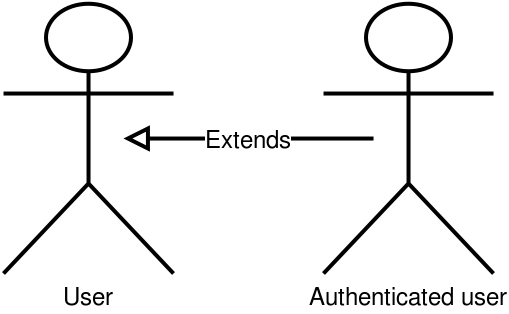
\includegraphics[scale=0.4]{img/Actors}

\end{centering}

\protect\caption{Actors}
\end{figure}



\subsubsection{User}

\begin{tabular}{|>{\centering}p{0.15\textwidth}|>{\raggedright}p{0.8\textwidth}|}
\hline 
 & User\tabularnewline
\hline 
Description & A user the system is able to check on its security scheme, it's somehow
\emph{registered } on the system.\tabularnewline
\hline 
\end{tabular}


\subsubsection{Authorized user}

\begin{tabular}{|>{\centering}p{0.15\textwidth}|>{\raggedright}p{0.8\textwidth}|}
\hline 
 & Anonymous user\tabularnewline
\hline 
Description & A user the system knows nothing about.\tabularnewline
\hline 
\end{tabular}


\subsubsection{Use cases}

Use cases describe the steps (and its deviations) to complete a certain
operation in the system.


\subsubsection{Read a collection}

\begin{tabular}{|>{\centering}p{0.15\textwidth}|>{\raggedright}p{0.8\textwidth}|}
\hline 
 & Read a collection\tabularnewline
\hline 
Actors & User or Anonymous user\tabularnewline
\hline 
Description & \tabularnewline
\hline 
Main scenario & \begin{enumerate}
\item A user clicks on a specific directory.
\item DPM server checks and accepts the request.\end{enumerate}
\tabularnewline
\hline 
Alternative flow & \begin{description}
\item [{2a}] The user is not allowed to perform that operation.\end{description}
\tabularnewline
\hline 
\end{tabular}


\subsubsection{Create a collection}

\begin{tabular}{|>{\centering}m{0.15\textwidth}|>{\raggedright}p{0.8\textwidth}|}
\hline 
 & Create a collection\tabularnewline
\hline 
Actors & User or Anonymous user\tabularnewline
\hline 
Description & \tabularnewline
\hline 
Main scenario & \begin{enumerate}
\item A user clicks on new directory button.
\item The user writes a collection name.
\item DPM server checks the name and accepts the request.\end{enumerate}
\tabularnewline
\hline 
Alternative flow & \begin{description}
\item [{2a}] The user cancels the operation.
\item [{3a}] The user is not allowed to perform that operation.
\item [{3b}] The given name is not valid.\end{description}
\tabularnewline
\hline 
\end{tabular}


\subsubsection{Delete a collection}

\begin{tabular}{|>{\centering}p{0.15\textwidth}|>{\raggedright}p{0.8\textwidth}|}
\hline 
 & Delete a collection\tabularnewline
\hline 
Actors & User or Anonymous user\tabularnewline
\hline 
Description & \tabularnewline
\hline 
Main scenario & \begin{enumerate}
\item A user clicks on delete directory button.
\item The user confirms the deletion.
\item DPM server checks and accepts the request.\end{enumerate}
\tabularnewline
\hline 
Alternative flow & \begin{description}
\item [{2a}] The user cancels the operation.
\item [{3a}] The user is not allowed to perform that operation.\end{description}
\tabularnewline
\hline 
\end{tabular}


\subsubsection{Download a file}

\begin{tabular}{|>{\centering}p{0.15\textwidth}|>{\raggedright}p{0.8\textwidth}|}
\hline 
 & Download a file\tabularnewline
\hline 
Actors & User or Anonymous user\tabularnewline
\hline 
Description & \tabularnewline
\hline 
Main scenario & \begin{enumerate}
\item A user clicks on download button.
\item The user selects the location to save the file.
\item DPM server checks and accepts the request.\end{enumerate}
\tabularnewline
\hline 
Alternative flow & \begin{description}
\item [{2a}] The user cancels the operation.
\item [{3a}] The user is not allowed to perform that operation.\end{description}
\tabularnewline
\hline 
\end{tabular}


\subsubsection{Upload a file}

\begin{tabular}{|>{\centering}p{0.15\textwidth}|>{\raggedright}p{0.8\textwidth}|}
\hline 
 & Upload a file\tabularnewline
\hline 
Actors & User or Anonymous user\tabularnewline
\hline 
Description & \tabularnewline
\hline 
Main scenario & \begin{enumerate}
\item A user clicks on upload button.
\item The user selects the file(s) to upload.
\item DPM server checks and accepts the request.\end{enumerate}
\tabularnewline
\hline 
Alternative flow & \begin{description}
\item [{2a}] The user cancels the operation.
\item [{3a}] The user is not allowed to perform that operation.\end{description}
\tabularnewline
\hline 
\end{tabular}


\subsubsection{Delete a file}

\begin{tabular}{|>{\centering}p{0.15\textwidth}|>{\raggedright}p{0.8\textwidth}|}
\hline 
 & Delete a file\tabularnewline
\hline 
Actors & User or Anonymous user\tabularnewline
\hline 
Description & \tabularnewline
\hline 
Main scenario & \begin{enumerate}
\item A user clicks on delete button.
\item The user confirms the deletion.
\item DPM server checks and accepts the request.\end{enumerate}
\tabularnewline
\hline 
Alternative flow & \begin{description}
\item [{2a}] The user cancels the operation. 
\item [{3a}] The user is not allowed to perform that operation.\end{description}
\tabularnewline
\hline 
\end{tabular}


\subsection{Domain data conceptual model}

This model is drawn from the information requirements. A conceptual
UML class diagram, in figure~\ref{fig:conceptualdatamodel}, is developed,
identifying classes, attributes, relationships, additional restrictions
and derivation rules, if any. 


\subsubsection{Files}

\begin{tabular}{|>{\centering}p{0.15\textwidth}|>{\raggedright}p{0.8\textwidth}|}
\hline 
\strong{Attribute} & \strong{Description}\tabularnewline
\hline 
Filename & The name of the file (including extension).\tabularnewline
\hline 
Size & The file size, in KB.\tabularnewline
\hline 
Modification date & The last date the file has been altered.\tabularnewline
\hline 
Metalink & The metalink information (actual hosting server, alternate locations...)\tabularnewline
\hline 
\end{tabular}


\subsubsection{Collections}

\begin{tabular}{|>{\centering}p{0.15\textwidth}|>{\raggedright}p{0.8\textwidth}|}
\hline 
\strong{Attribute} & \strong{Description}\tabularnewline
\hline 
Name & The name of the collection in the system.\tabularnewline
\hline 
Path & The router of the collection, starting from the server root.\tabularnewline
\hline 
Children collections & The list of collections within another one.\tabularnewline
\hline 
Files contained & The list of files inside that directory.\tabularnewline
\hline 
Expanded & It indicates if the collection node is expanded in the tree or not.\tabularnewline
\hline 
First parent & Tells if the node is the top element on the route.\tabularnewline
\hline 
\end{tabular}

\begin{figure}
\begin{centering}\label{fig:conceptualdatamodel}

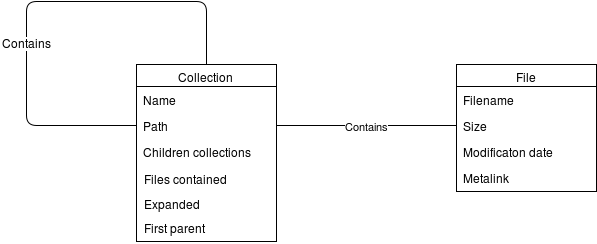
\includegraphics[width=0.8\textwidth]{img/ConceptualDataModel}

\end{centering}

\protect\caption{Domain data conceptual model}
\end{figure}



\subsection{Behavioural Model}

Not all possible sequence diagrams are shown (different use cases
and scenarios), we present a small sample that may be representative
of the the whole system:


\subsubsection{Create a collection}

\begin{figure}[h]
\begin{centering}

\label{fig:seqcreatecoll}

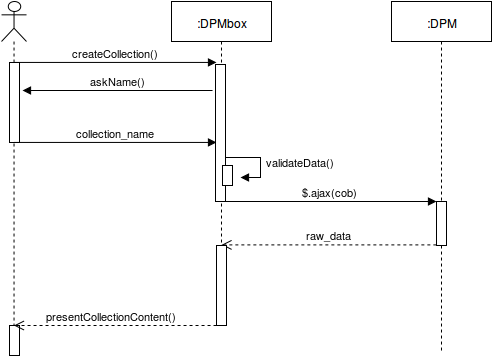
\includegraphics[width=0.6\textwidth]{img/SeqDiagram_CreateCollection}

\end{centering}

\protect\caption{Sequence diagram, create collection}


\end{figure}

\begin{enumerate}
\item A user clicks on new directory button.
\item DPMbox shows a text box asking for a name.
\item The user writes a collection name.
\item DPMbox validates the name.
\item DPMbox send the new collection request to the server.
\item DPM server checks and responds to the request.
\item DPMbox present the information to the user.
\end{enumerate}

\subsubsection{Download file}

\begin{figure}[h]
\begin{centering}

\label{fig:seqdnlfile}

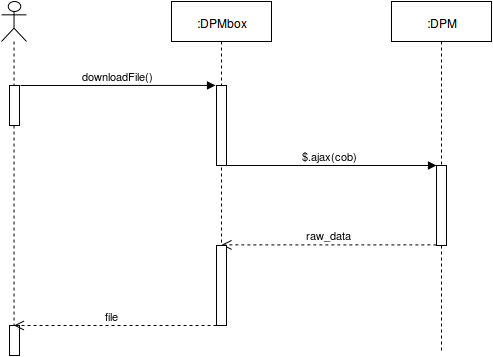
\includegraphics[width=0.6\textwidth]{img/SeqDiagram_DownloadFile}

\end{centering}

\protect\caption{Sequence diagram, download file}
\end{figure}

\begin{enumerate}
\item A user clicks on download button.
\item DPMbox send the download request to the server.
\item DPM server checks and responds to the request.
\item DPMbox present the file to the user.
\item The user selects the location to save the file.
\end{enumerate}

\subsubsection{Delete file}

\begin{figure}[h]
\begin{centering}

\label{fig:seqdeletefile}

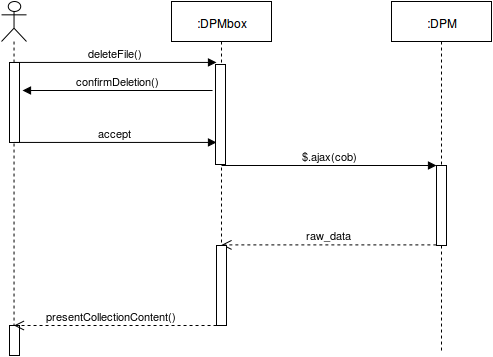
\includegraphics[width=0.6\textwidth]{img/SeqDiagram_DeleteFile}

\end{centering}

\protect\caption{Sequence diagram, delete file}
\end{figure}

\begin{enumerate}
\item A user clicks on delete button.
\item DPMbox shows the confirm deletion message.
\item The user confirms the deletion.
\item DPMbox send the deletion request to the server.
\item DPM server checks and responds to the request.
\item DPMbox present the information to the user.
\end{enumerate}

\subsection{User interface model}

This section provides an approximation to the appearance and navigation
through the user interface.


\subsubsection{Navigation model}

In the navigation model we can see that the main operation in DPMbox
is \emph{read collection}, this is so because after almost every
other operation the collection state is altered, so the content must
be checked again. This only not happens with the download functionality,
since the contents in the collection doesn't change after this operation.

\begin{figure}[h]
\begin{centering}

\label{fig:navmodel}

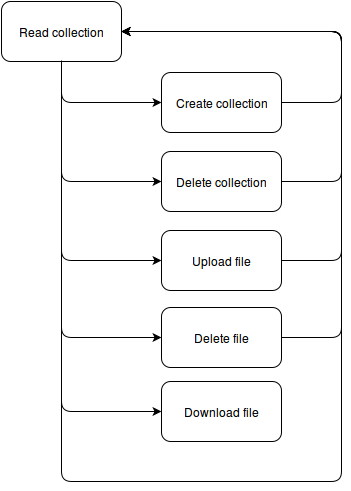
\includegraphics[width=0.4\textwidth]{img/NavigationDiagram}

\end{centering}

\protect\caption{Navigation model}
\end{figure}



\subsubsection{Prototypes}

You can check some sketched views of the user interface design with
the prototypes shown on figures~\prettyref{fig:intschememain} (main
screen),~\prettyref{fig:intschemeaction} (action required screen)
and~\prettyref{fig:intschemeerror} (error detected screen).

\begin{figure}[h]
\begin{centering}

\label{fig:intschememain}

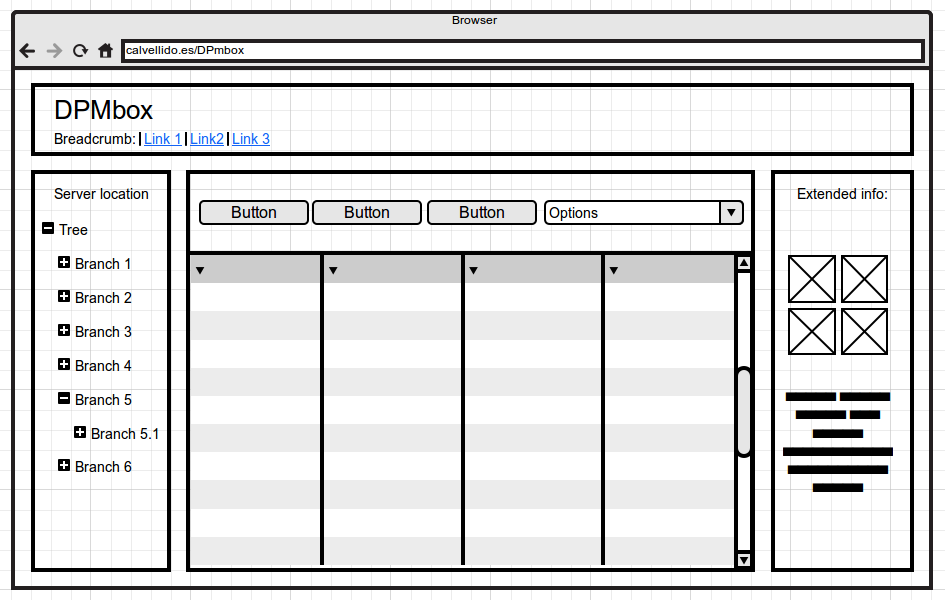
\includegraphics[width=1\textwidth]{img/design_scheme}

\end{centering}

\protect\caption{Interface design, main scheme}
\end{figure}


\begin{figure}[h]
\begin{centering}

\label{fig:intschemeaction}

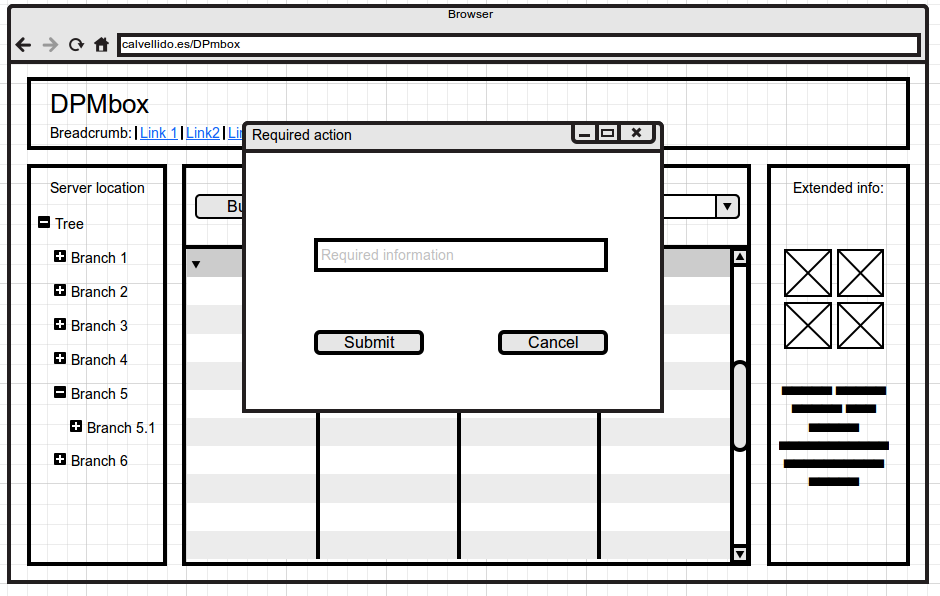
\includegraphics[width=1\textwidth]{img/design_action}

\end{centering}

\protect\caption{Interface design, action required}
\end{figure}


\begin{figure}[h]
\begin{centering}

\label{fig:intschemeerror}

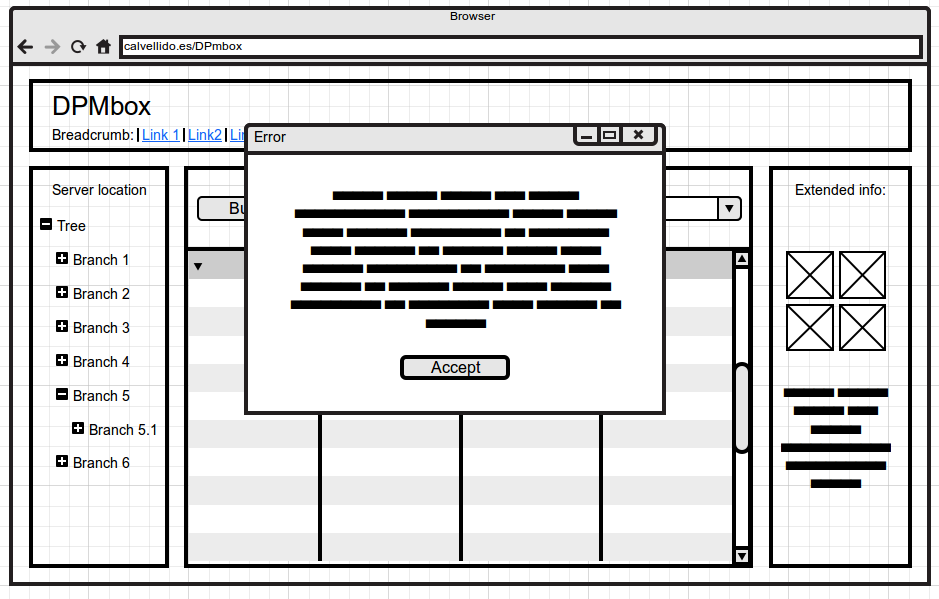
\includegraphics[width=1\textwidth]{img/design_error}

\end{centering}

\protect\caption{Interface design, error}
\end{figure}



\section{System design~\label{sec:System-design}}

DPMbox design has followed a minimal viable product approach, being
started as a WebDAV connection interface and then being adapted to
DPM specifications. It's been constructed modularly and could be basically
divided in two parts: the web user interface and the JavaScript API
that communicates with the server. 


\subsection{Logic architecture}

Schuldt in~\cite{reference_db_Schuldt09a} defines a multi-tier architecture
as 
\begin{quotation}
\emph{“A software architecture in which different software components, organized
in tiers (layers), provide dedicated functionality. The most common
occurrence of a multi-tier architecture is a three-tier architecture
consisting of a data management tier (mostly encompassing one or several
data- base servers), an application tier (business logic) and a client
tier (interface functionality). Novel deployments come with additional
tiers. Web information systems, for instance, encompass a dedicated
tier (web tier) between client and application layer. Conceptually,
a multi-tier architecture results from a repeated application of the
client/server paradigm. A component in one of the middle tiers is
client to the next lower tier and at the same time acts as server
to the next higher tier.”}
\end{quotation}


A three tier architecture is a very common architecture. It's typically
split into a presentation or GUI tier, an application logic tier,
and a data tier. An example can be seen on figure

\begin{figure}
\begin{centering}

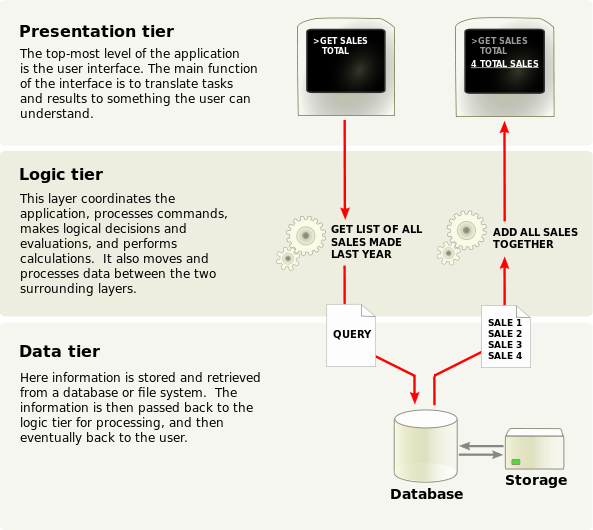
\includegraphics[width=1\textwidth]{img/Three-tier_application}

\end{centering}

\protect\caption{Visual overview of a Three-tiered application}
\end{figure}


The presentation or GUI tier contains the user interface of the application.
The presentation tier is \emph{dumb}, meaning it does not make any
application decisions. It just forwards the user's actions to the
application logic tier. If the user needs to enter information, this
is done in the presentation tier too.

The application logic tier makes all the application decisions. This
is where the business logic is located. The application logic knows
what is possible and what is allowed to do in the system. The application
logic reads and stores data into the data tier.

The data tier stores the data used in the application. The data tier
can typically store data safely, perform transactions or search through
large amounts of data quickly. 

The purpose of multitier architectures is to insulate the different
layers of the application from each other. The GUI client doesn't
know how the server is working internally, and the server doesn't
know how the database server works internally. They just communicate
via standard interfaces.

Web applications specially have another advantage. If you make updates
to the GUI client or the application logic running on the server,
all clients get the latest updates the next time they access the application.
The browser downloads the updated client, and the updated client accesses
the updated server. 

DPMbox is integrated into the DPM software stack. Thus, it must be
analyzed in that context, showing us that it is just another layer
of the whole system. This can be seen on~\ref{fig:logicscheme}.
The DPMbox layer doesn't know any operating details of the DPM layer,
they just connect trough a common interface, in this case a WebDAV
interface.

\begin{figure}[h]
\begin{centering}

\label{fig:logicscheme}

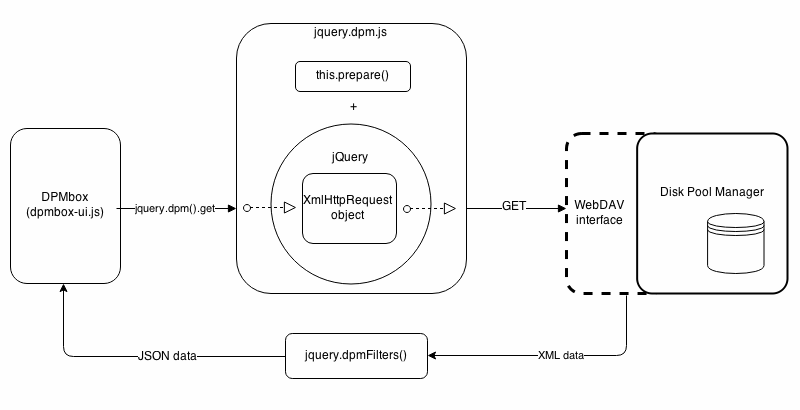
\includegraphics[width=1\textwidth]{img/DPMbox_globalscheme}

\end{centering}

\protect\caption{DPMbox logic scheme}
\end{figure}



\subsection{Physical architecture}

In this section, we describe the major hardware components that are
present in the physical architecture of our system. Again, for the
physical view, DPMbox can't be detached from the DPM architecture.
Physically a DPM server can be a group of machines or even just one,
but in a global view the physical architecture is a typical client-server
model. This is represented in figure~\ref{fig:physarch}.

\begin{figure}[h]
\begin{centering}\label{fig:physarch}

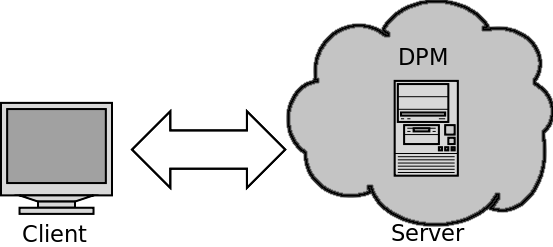
\includegraphics[width=0.5\textwidth]{img/Client-Server}

\end{centering}

\protect\caption{DPMbox physical architecture}
\end{figure}



\subsubsection{DPM server}

Apart from the special case of a purely test setup, is recommended
that a DPM server provides (at least):
\begin{itemize}
\item 2Ghz processor with 512MB of memory (not a hard requirement) 
\item Dual power supply 
\item Mirrored system disk 
\item Database backups 
\item It will usually runs on Scientific Linux, and the WebDAV interface
(including DPMbox view) is offered through Apache
\end{itemize}

\subsubsection{Client access}

The non-functional requirement NRQ-6, in~\prettyref{tab:portability}
indicates that the web platform should be accessible from any kind
of operating system through a web browser. Thus, the only restriction
to users is having a modern web browser that provides access and supports
the latest web standards.


\subsection{DPMbox WebDAV communication}

Taking the former DPM HTTP/WebDAV frontend implementation, the first
step in the development process was to build an API with JavaScript
that can interact with it. That API uses AJAX calls to perform the
HTTP/WebDAV requests and receives the data in an \ac{XHR} object.
This way it's possible to expose WebDAV standard methods like PROPFIND
or MKCOL and use the information provided by them in an HTML or any
other type of document through JavaScript and jQuery. 

What the library offers is (method with its corresponding WebDAV call
in brackets): 


\subsubsection{HTTP verbs}
\begin{description}
\item [{get}] (GET) 
\item [{post}] (POST) 
\item [{head}] (HEAD) 
\item [{mkcol,~createFolder}] (MKCOL) 
\item [{put,~createFile}] (PUT) 
\item [{remove}] (DELETE) 
\item [{report}] (REPORT) 
\item [{getVersionTreeReport}] (REPORT) 
\item [{checkout}] (CHECKOUT) 
\item [{uncheckout}] (UNCHEKCOUT) 
\item [{checkin}] (CHECKIN) 
\item [{versionControl}] (VERSION-CONTROL) 
\item [{lock}] (LOCK) 
\item [{unlock}] (UNLOCK) 
\item [{propfind,~getProperty}] (PROPFIND) 
\item [{proppatch,~setProperty,~removeProperty}] (PROPPATCH)
\end{description}
Besides the main verbs, the library takes care of global data as XML
headers and defines some additional methods.


\subsubsection{Additional methods}
\begin{description}
\item [{isCollection:}] Returns whether an element is a collection or not
by looking for a collection XML tag inside a resourcetype property.
For a DPM server there’s no need to use it since a DPM response includes
a specific property \code{iscollection} to check this, but the method
is needed for standard WebDAV server support.
\item [{getNodesByTag:}] Works exactly like the standard \code{getElementsByTagName},
however introduces the ability to filter those results by namespace,
which is important for handling WebDAV results.
\item [{seekToNode:}] Sets resource variable to first node matched via
\code{getNodesByTag}, and returns this, allowing further processing.
\item [{eachNode:}] Executes a function on each element.
\item [{nodeText:}] Get the text contained by a node.
\item [{nodeName:}] Returns the name of a node (the tag name, essentially).
\item [{extendbeforesend:}] jQuery.ajax option \code{beforeSend} may be
set to a function reference, and this function will fire prior to
the request being sent. It gets the XHR object, so this is the point
you will want to do things like set headers, for example.
\item [{prepare:}] Prepares the WebDAV call. Here we want to ensure integrity
of call object, verify WebDAV method requested, set any authorization
information (if necesssary), and return the modified call object.
WebDAV servers usually respond in XML but some WebDAV methods will
not return anything at all, or return an empty response. This matters
to jQuery in that the success method of a jQuery.ajax options object
won’t fire if the reponse could not be parsed (although the complete
method will). Is needed to be aware of what \code{dataType} of your
AJAX response will be, and set it appropriately.
\end{description}

\subsection{Files upload and redirection}

In the DPM architecture one entity handles the namespace with the
metadata, and other ones store the files with the actual data. This
means that any request must go through a server hosting the namespace
first, and then redirect to the disk node storing the physical file.
We execute a PUT call and the file won’t be yet uploaded but DPM will
answer back, then our web application has to try a second time. The
URL needed to actually do the PUT would look like this, you can see
the specific DPM node where the file will be uploaded, including a
token validating the transaction:
\begin{verbatim}
http://lxfsra04a04.cern.ch/srv/dpm/01/nogroup/2015-03-02/XHR.js.zip.2900489
.0?sfn=%2Fdpm%2Fcern.ch%2Fhome%2Fdteam%2Faalvarez%2Fpublic%2Fcollection_d
%2FXHR.js.zip&dpmtoken=dbf5fcbe-7c31-4849-aa57-b07c6b474f5e&token=ojkU%2
FdgyPqTYEvu4TfZAyueVDqQ%3D%401425288602%401
\end{verbatim}
\begin{figure}[H]
\begin{centering}\label{fig:redirection}

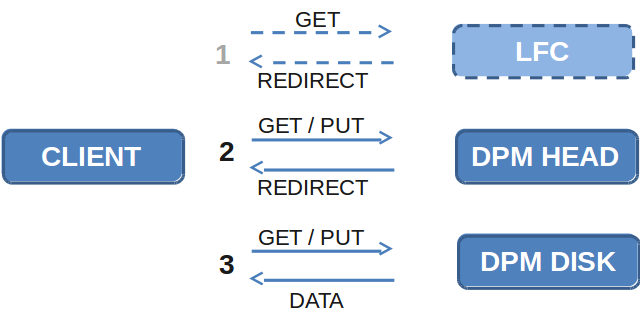
\includegraphics[width=0.4\textwidth]{img/redirection}

\end{centering}

\protect\caption{DPM redirection process}
\end{figure}


User agents commonly apply same-origin restrictions to network requests.
These restrictions prevent a client-side Web application as DPMbox
running from one origin from obtaining data retrieved from another
origin, and also limit unsafe HTTP requests that can be automatically
launched toward destinations that differ from the running application’s
origin. In user agents that follow this pattern, network requests
typically include user credentials with cross-origin requests, including
HTTP authentication and cookie information. As DPMbox relies heavily
on XHR (XML Http Request) calls this has to be handled carefully.

You can check a bit of history of XHR and CORS (Cross-Origin Resource
Sharing) and why this is happening on~\cite{1_cruz_2015}.

In early stages of the development, the DPM initial behaviour was
to answer with a 302 code indicating redirection, and then the browser
will try transparently to reach that new location. That would work
it out, but the thing is that 30x responses are treated as error by
CORS specification~\cite{W3C:CORS}:
\begin{quote}
\emph{This is the actual request. Apply the make a request steps and observe
the request rules below while making the request.\\
\\
If the response has an HTTP status code of 301, 302, 303, 307, or
308 Apply the cache and network error steps.\\
\\
(…)\\
\\
Whenever the network error steps are applied, terminate the algorithm
that invoked this set of steps and set the cross-origin request status
to network error.\\
\\
Note: This has no effect on setting of user credentials. I.e. if the
block cookies flag is unset, cookies will be set by the response.\\
\\
Whenever the cache and network error steps are applied, follow these
steps:\\
Remove the entries in the preflight result cache where origin field
value is a case-sensitive match for source origin and URL field value
is a case-sensitive match for request URL.\\
\\
Apply the network error steps acting as if the algorithm that invoked
the cache and network error steps invoked the network error steps
instead.}
\end{quote}
So with this configuration it would be impossible to get any information
of the response, not any header at a JavaScript level, specifically
the \code{Location} header. Finally, the solution given was manage
the uploads though a first empty PUT including a header \code{X-No-Redirect}
and the server will answer with a \code{202 Accepted} response. We
can extract any header from this type of response as it’s not treated
as error for XHR CORS requests.

After that we have to include this header information to our server
CORS security settings and add it to the directive \code{Access-Control-Expose-Headers.}
In short, it's necessary to configure the DPM server to response with
the headers included on~\prettyref{lis:Access-Control-Configuration-1}.
\begin{verse}
\begin{lstlisting}[caption={Access-Control Configuration},label={lis:Access-Control-Configuration-1},float,basicstyle={\footnotesize\ttfamily},columns=fullflexible]
Access-Control-Allow-Origin: UrlWhereDPMboxIsHosted.host 
Access-Control-Allow-Credentials: true 
Access-Control-Allow-Methods: ACL, CANCELUPLOAD, CHECKIN, CHECKOUT, COPY, DELETE, GET, HEAD, LOCK, MKCALENDAR, MKCOL, MOVE, OPTIONS, POST, PROPFIND, PROPPATCH, PUT, REPORT, SEARCH, UNCHECKOUT, UNLOCK, UPDATE, VERSION-CONTROL 
Access-Control-Allow-Headers: Authorization, Overwrite, Destination, Content-Type, Depth, User-Agent, Translate, Range, Content-Range, Timeout, X-File-Size, X-Requested-With, Accept, Accept-Version, If-Modified-Since, X-File-Name, Cache-Control, Location, Lock-Token, If, X-No-Redirect 
Access-Control-Expose-Headers: DAV, content-length, Allow, Location
\end{lstlisting}

\end{verse}

\subsection{User interface\label{sub:User-interface}}

As said by Donal Norman~\cite{Norman02}:
\begin{quote}
“\emph{When a device as simple as a door has to come with an instruction
manual—even a one-word manual—then it is a failure, poorly designed.
.}
\end{quote}


As one of the main objectives of DPMbox was to attract new users to
the system, the user interface design must be very easy to user appealing
to the final user. Following Mandel Golden rules of User Interface
Design~\cite{Mandel1997}:
\begin{itemize}
\item Place Users in Control 
\item Reduce Users' Memory Load 
\item Make the Interface Consistent
\end{itemize}


A way to accomplish this goals is to make the GUI quite similar to
the common file browsers that most people are used to.

\strong{Usability} is the extent to which a product can be used by
specified users to achieve specified goals with effectiveness, efficiency
and satisfaction in a specified context of use.

The concept of usability is defined of the ISO 9241 standard by effectiveness,
efficiency, and satisfaction of the user. Part 11~\cite{iso9241-11}
gives the following definition of usability: 
\begin{itemize}
\item Usability is measured by the extent to which the intended goals of
use of the overall system are achieved (effectiveness). 
\item The resources that have to be expended to achieve the intended goals
(efficiency). 
\item The extent to which the user finds the overall system acceptable (satisfaction). 
\end{itemize}


\strong{Accessibility} of a system describes its ease of reach, use
and understanding. In terms of user experience design it can also
be related to the overall comprehensibility of the information and
features. It contributes to shorten the learning curve attached with
the system. Accessibility in many contexts can be related to the ease
of use for people with disabilities and comes under usability.

The information presentation is described in Part 12 of the ISO 9241~\cite{iso9241-12}
standard for the organization of information (arrangement, alignment,
grouping, labels, location), for the display of graphical objects,
and for the coding of information (abbreviation, color, size, shape,
visual cues) by seven attributes. The “attributes of presented information”
represent the static aspects of the interface and can be generally
regarded as the “look” of the interface. The attributes are detailed
in the recommendations given in the standard. Each of the recommendations
supports one or more of the seven attributes. The seven presentation
attributes are: 
\begin{itemize}
\item Clarity: the information content is conveyed quickly and accurately. 
\item Discriminability: the displayed information can be distinguished accurately. 
\item Conciseness: users are not overloaded with extraneous information. 
\item Consistency: a unique design, conformity with user’s expectation. 
\item Detectability: the user’s attention is directed towards information
required. 
\item Legibility: information is easy to read. 
\item Comprehensibility: the meaning is clearly understandable, unambiguous,
interpretable, and recognizable. 
\end{itemize}


\strong{User~guidance} appears in Part 13 of the ISO 9241~\cite{iso9241-13}
standard, it describes that information should be readily distinguishable
from other displayed information and should be specific for the current
context of use. User guidance can be given by the following five means: 
\begin{itemize}
\item Prompts indicating explicitly (specific prompts) or implicitly (generic
prompts) that the system is available for input. 
\item Feedback informing about the user’s input timely, perceptible, and
non-intrusive. 
\item Status information indicating the continuing state of the application,
the system’s hardware and software components, and the user’s activities. 
\item Error management including error prevention, error correction, user
support for error management, and error messages. 
\item On-line help for system-initiated and user initiated requests with
specific information for the current context of use. 
\end{itemize}

\subsubsection{Sketch}

Thereby, the GUI of DPMbox has been designed following these guidelines.
In the figure~\ref{fig:design_prototype} you can see an initial
prototyped design. Upon a layout divided in a top panel and three
horizontal ones under it you can find the sidebar managing the directory
tree, a grid in the center showing the files including a toolbar,
and then in the right panel there is the directory information. 

\begin{figure}
\begin{center}\label{fig:design_prototype}

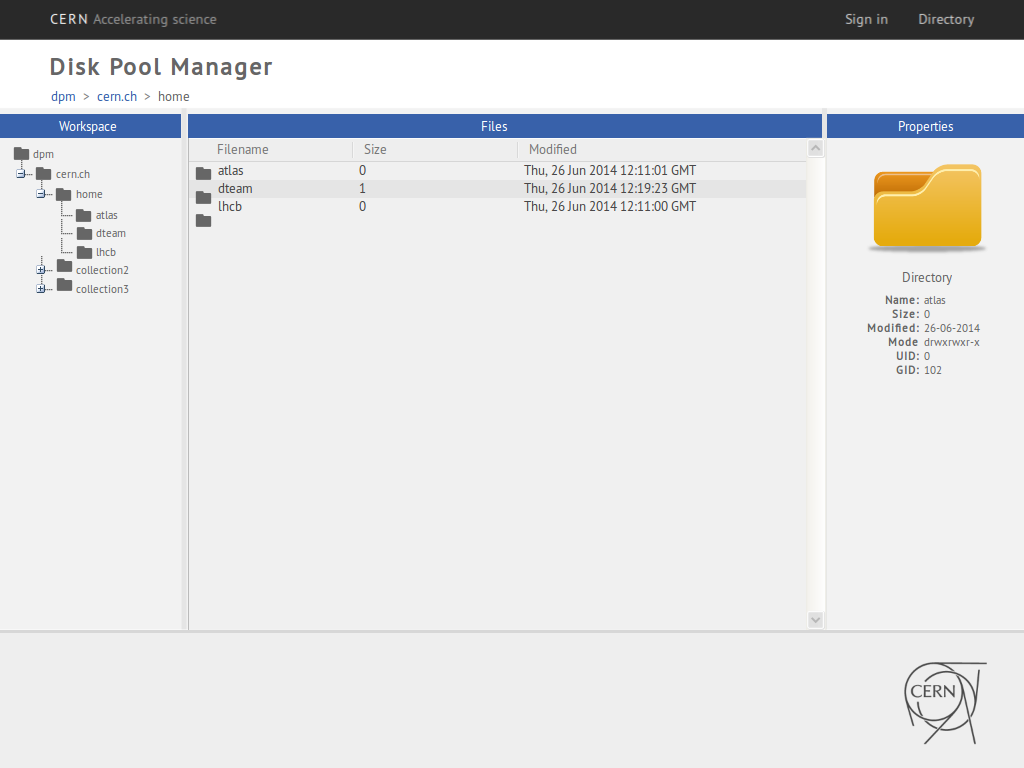
\includegraphics[width=1\textwidth]{img/DPMbox_interface_sketch}

\end{center}

\protect\caption{DPMbox design prototype}
\end{figure}



\section{Libraries and tools}


\subsection{Version control\label{sub:Version-control}}

Git has been used, getting advantage of the GitHub platform. Git is
a distributed revision control system with an emphasis on speed, data
integrity, and support for distributed, non-linear workflows.Git was
initially designed and developed by Linus Torvalds for Linux kernel
development in 2005, and has since become one of the most widely adopted
version control systems for software development.

The DPMbox repository can be checked (and forged!) on~\cite{11_valencia_calvellido_2015}.


\subsection{Program languages and technologies\label{sub:Program-languages-and}}


\subsubsection{HTML }

HTML (Hyper Text Markup Language) is the text markup language normally
used in World Wide Web (WWW). It was created by Tim Berners-Lee (former
CERN researcher) in 1986 from two existing tools: the concept of hypertext
and SGML. HTML allows you to define both the structure and location
of the items displayed on a Web page and the relations between the
different components of a Web site by using hyperlinks. The interpretation
of HTML documents is performed by Web browsers such as Mozilla Firefox
or Google Chrome and others. The interpretation may make the final
presentation vary in small details. Therefore the development of HTML
is adjusted to the maximum to the standards set by the W3C~\cite{2_w3.org_2015}.


\subsubsection{CSS}

The term CSS, which stands for Cascading Style Sheets, refers to the
formal language used to define the presentation of structured documents
written in HTML, XML and XHTML by extension. The World Wide Web Consortium
(W3C) is the agency responsible for developing the specification of
style sheets that serve as a standard for browsers. The objective
of CSS is separate the structure of a Web document from its visual
representation~\cite{3_w3.org_2015}.

The CSS from w2ui framework has been adapted accordingly to suit the
needs of DPMbox.


\subsubsection{JavaScript}

JavaScript is a high level, dynamic, untyped, and interpreted programming
language. It has been standardized in the ECMAScript language specification~\cite{EcmaScript}.
Alongside HTML and CSS, it is one of the three essential technologies
of World Wide Web content production; the majority of websites employ
it and it is supported by all modern web browsers without plug-ins.
JavaScript is prototype-based with first-class functions, making it
a multi-paradigm language, supporting object-oriented, imperative,
and functional programming styles. It has an API for working with
text, arrays, dates and regular expressions, but does not include
any I/O, such as networking, storage or graphics facilities, relying
for these upon the host environment in which it is embedded~\cite{4_mozilla_developer_network_2015}.

ECMAScript 6 includes interesting syntax and structural improvements
but it was in process of approval while DPMbox was being developed,
thus the standard followed has been ECMAScript 5.1~\cite{EcmaScript}.


\subsubsection{jQuery}

jQuery is a cross-platform JavaScript library designed to simplify
the client-side scripting of HTML. jQuery is the most popular JavaScript
library in use today, with installation on 65\% of the top 10 million
highest-trafficked sites on the Web~\cite{w3techs.com_2015}. jQuery
is free, open-source software licensed under the MIT License.

Version used in DPMbox development is version 2.1.3.


\subsubsection{w2ui}

W2UI is a small JavaScript UI library with a complete set of widgets
that covers a wide range of interface design elements: layout, grid,
sidebar, toolbar, tabs, fields, popup and other utilities. It has
been created by Vitali Malinouski and it's licensed under MIT license.
Some of its features are:
\begin{itemize}
\item Complete w2ui library is only 69kb (minified and gziped) and provides
extremely fast load and execution. It is 9 times smaller then ExtJS
and 7 times smaller then Kendo UI. It is just a bit over the size
of jQuery.
\item It’s really easy to use with simple and standard API methods, JSON
friendly, and it has a stable and good support from its main developer.
\item It has no dependencies except jQuery, is all-in-one solution. It contains
all most common UI widgets: layout, grid, sidebar, tabs, toolbar,
popup, field controls and forms. No need to put together a collection
of mismatched plugins or more libraries.
\item The library heavily uses HTML5 and CSS3 and yet supports all major
modern browsers. Latest Chrome, FireFox 7+, Safari 5+ and IE 9+ are
among supported browsers.
\end{itemize}
Version used by DPMbox is version 1.4.2..


\subsubsection{XML}

XML stands for eXtensible Markup Language, is a markup language developed
by the World Wide Web Consortium (W3C) used to store data in a human
readable form. It is proposed as a standard for exchanging structured
information between different platforms. 

WebDAV servers, which DPMbox relies on, answers all requests with
XML content.


\subsubsection{JSON}

JSON (JavaScript Object Notation) is an open standard format that
uses human-readable text to transmit data objects consisting of attribute–value
pairs. It is the primary data format used for asynchronous browser/server
communication (AJAJ), largely replacing XML (used by AJAX).

DPMbox UI uses JSON instead of XML, so the responses received from
the server are parsed and translated to JSON format.


\subsection{Tools \label{sub:Tools}}

As stated on section~\prettyref{sec:Non-Human-resources}, GNU/Linux
Ubuntu 10.04, and also GNU/Linux Mint 17 were the OS where DPMbox
has been developed.


\subsubsection{Apache}

The Apache HTTP Server is the world's most widely used web server
software. Originally based on the NCSA HTTPd server, development of
Apache began in early 1995 after work on the NCSA code stalled. Apache
played a key role in the initial growth of the World Wide Web, quickly
overtaking NCSA HTTPd as the dominant HTTP server, and has remained
most popular since April 1996. In 2009, it became the first web server
software to serve more than 100 million websites.

Version used for development has been version 2.2.14. On production
DPM servers Apache 2.2.15 is typically used.


\subsubsection{Geany}

Geany is a lightweight cross-platform GUI based text editor using
Scintilla and GTK+, including basic Integrated Development Environment
(IDE) features. It is designed to have short load times, with limited
dependency on separate packages or external libraries. It is available
for a wide range of operating systems, such as BSD, Linux, Mac OS
X, Solaris and Windows. Among the supported programming languages
and markup languages are C, C++, C\#, Java, JavaScript, PHP, HTML,
\LaTeX{}, CSS, Python, Perl, Ruby, Pascal, Haskell, Erlang, Vala and
many others.

Version used to develop DPMbox is 1.24.1.


\subsubsection{Firefox Developer Edition}

Firefox Developer Edition is a version of Firefox tailored for developers,
featuring the latest Firefox features and experimental developer tools.
It provides easy accessibility for a wide array of developer tools
which help in making debugging easy and help in faster and more professional
development. Tools include Valence, WebIDE, Page Inspector, Web Console,
JavaScript Debugger, Network Monitor...

Version used has been version 35.0a2.


\subsubsection{Firebug}

Firebug is a free and open-source web browser extension for Mozilla
Firefox that facilitates the live debugging, editing, and monitoring
of any website's CSS, HTML, DOM, XHR, and JavaScript. Firebug is licensed
under the BSD license and was initially written in January 2006 by
Joe Hewitt, one of the original Firefox creators. The Firebug Working
Group oversees the open source development and extension of Firebug.
It has two major implementations: an extension for Mozilla Firefox
and a bookmarklet implementation called Firebug Lite which can be
used with Google Chrome. In addition to debugging web pages, Firebug
is a useful tool for web security testing and web page performance
analysis.

Versions used have been verison 1.114b1 and version 2.0.12.


\subsubsection{JSHint}

JSHint is a static code analysis tool used in software development
for checking if JavaScript source code complies with coding rules.
It was forked from Douglas Crockford's JSLint project, as it was felt
that the original did not allow enough customization options. 

This tool has been used to ensured the good quality of the written
code. It was used through Geany and Firefox Developer Edition with
version used being version 2.4.0.


\section{Implementation}


\subsection{HTML}


\subsubsection{index.html}

It is actually just a container for the JavaScript generated interface.


\subsection{CSS}


\subsubsection{w2ui.css}

w2ui UI framework styles sheet.


\subsubsection{style.css}

Some rules indicating size, font and colors for the DPMbox interface
appearance and a slight overriding over some w2ui CSS rules to adapt
them accordingly.


\subsection{JavaScript}


\subsubsection{config.js}

A file to store the server and other configuration values that could
arise in the future.


\subsubsection{dpmbox-ui.js }

The user interface, constructed over the w2ui library. In this file
we use the data obtained through jquery.dpm.js, after being parsed
and translated to JSON by a method of jquery.dpmFilters.js. Considering
that is a petition on the network, the way to use it is by taking
advantage of jQuery AJAX callbacks, i.e. a success response. The listing~\prettyref{lis:jquery.dpm.js---GET-usage}
would represent what happens here.


\subsubsection{jquery.dpm.js }

This is the \emph{API}, or the library that actually communicates
with the DPM server dealing with the HTTP/WebDAV frontend. Through
this library we can use methods of the WebDAV standard like PROPFIND
or MKCOL in an HTML environment and thus manage the information they
provide. This API use XMLHttpRequest operations, also known as XHR.
These are basically AJAX calls that perform the HTTP/WebDAV requests
and receive the data in a JavaScript XHR object. An XMLHttpRequest
support GET, POST, PUT, and basically any HTTP method, and is available
in any browser, even in old ones like Internet Explorer 6 or Firefox
3.

In~\prettyref{lis:jquery.dpm.js---GET} we show a simplified version
of the API, a GET example is shown but the other verbs are are implemented
in a similar way, though considering some particularities (like the
PROPFIND needing a depth parameter). 

\begin{lstlisting}[caption={jquery.dpm.js - GET},label={lis:jquery.dpm.js---GET},language=Java,float,basicstyle={\footnotesize\ttfamily},columns=fullflexible]
$.fn.extend($,{ 	
	dpm: function(res) { 		
		var api = function() {
			this.get = function(cob) { 				
				this.prepare(cob, 'GET'); 				
				return this.send(cob); 			
			};
			this.prepare = function(cob, typ) { 				
				cob = cob || {}; 				
				cob.url = resourceUrl; 			
				cob.headers = cob.headers || {};
				cob.type = typ || 'GET'; 				
				cob.dataType  = cob.dataType || 'xml'; 			
			};
			this.send = function(cob) { 				
				lastRequest = $.ajax(cob); 				
				return lastRequest; 			
			};
		}; 		
		return new api;     
	} 
};
\end{lstlisting}


\code{cob} is the jQuery AJAX call object, in the prepare function
the DAV call is built. There it’s needed to ensure integrity of the
call object, verify the DAV method requested and set any authorization
information (if necessary). The headers that will include that information
are set by the \code{SetRequestHeader} AJAX method. After that, the
\code{send} function does the actual HTTP send through an AJAX request.

To use this API in an HTML document we just call the function needed,
which as we have seen is basically an AJAX call that we can process
if it success. In~\prettyref{lis:jquery.dpm.js---GET-usage} there
is an example reading an XML file and other one creating a test collection: 

\begin{lstlisting}[caption={jquery.dpm.js - GET usage},label={lis:jquery.dpm.js---GET-usage},language=Java,float,basicstyle={\footnotesize\ttfamily},columns=fullflexible]
// #get 
$.dpm(url + 'testxml.xml').get({ 	
	complete: function() { 		
		console.log('#get'); 	
	}, 	
	success:  function(dat, stat) { 		
		console.log(jQuery.dpm(dat).getNodesByTag('acl')); 	
	} 
});
//#mkcol 
$.dpm(url + 'test').mkcol({ 	
	complete:  function(dat, stat) { 		
		console.log('#mkcol'); 	}, 	
	async: false 
});

/* 
 * A proper call, setting the (firstly parsed) data on the interface
 * A function to refresh the grid content  
 */ 
function refreshContent(directory_route){     
	$.dpm(server + directory_route).readFolder({         
		success:    function(dat) {             
			w2ui.grid.clear();             
			w2ui.grid.add(dat);         },         
		dataFilter: $.dpmFilters.filesDPM     
	}); 
}
\end{lstlisting}


In the API there are also other methods developed in order to work
properly with the data, as seen on listing~\prettyref{lis:jquery.dpm.js---Additional}.
For example to traverse the nodes received in a PROPFIND, or to select
a specific property. 

\begin{lstlisting}[caption={jquery.dpm.js - Additional method},label={lis:jquery.dpm.js---Additional},language=Java,float,basicstyle={\footnotesize\ttfamily},columns=fullflexible]
this.getAllProperties = function(cob) { 	
	cob.data = XmlHeader + '<D:propfind xmlns:D="DAV:"><D:allprop/>';
	if(isArray(cob.includes)) { 		
		cob.data    +=  '<D:include>';
		for(var i=0; i < d.includes.length; i++) { 			
			cob.body  += '<D:' + d.includes[i] + '/>'; 		
		}
		cob.data    +=  '</D:include>'; 	
	}
	cob.data      += '</D:propfind>'; 	
	return this.propFind(cob); 
};
\end{lstlisting}



\subsubsection{jquery.dpmFilters.js}

WebDAV answers with XML data and the DPMbox interface understands
JSON, therefore some parsers are needed, and they are located in this
file. One of these filters can be checked on~\prettyref{lis:jquery.dpmFilters.js}.
A typical XML response of the server can be analyzed on listing~\prettyref{lis:xmlresponse}.

\begin{lstlisting}[caption={jquery.dpmFilters.js},label={lis:jquery.dpmFilters.js},language=Java,float,basicstyle={\footnotesize\ttfamily},columns=fullflexible]
(function($) { 
	$.fn.extend($,{ dpmFilters: { 			
		/* Returns an array of contained nodes not collections*/
		files: function(dat) {
			var davTree = [];
			$.dpm(dat).seekToNode('response').eachNode(function(node_response) {
				if (!$.dpm(node_response).isCollection())
					davTree.push(node_response);                  					
			});                  					
			return davTree;              			
		}          		
	}});
})(jQuery); 
\end{lstlisting}


\begin{lstlisting}[caption={XML response},label={lis:xmlresponse},language=XML,float,basicstyle={\footnotesize\ttfamily},columns=fullflexible]
<D:multistatus xmlns:D="DAV:" xmlns:ns0="DAV:"> 	
	<D:response xmlns:lcgdm="LCGDM:" xmlns:lp3="LCGDM:" xmlns:lp1="DAV:" xmlns:lp2="http://apache.org/dav/props/"> 		<D:href>/dpm/cern.ch/home/dteam/aalvarez/public/test_collection/</D:href> 		
		<D:propstat> 			
			<D:prop> 				
				<lcgdm:type>0</lcgdm:type> 				
				<lp1:resourcetype> 					
					<D:collection></D:collection> 				
				</lp1:resourcetype> 				
				<lp1:creationdate>2015-04-04T09:51:59Z</lp1:creationdate> 				
				<lp1:getlastmodified>Fri, 27 Feb 2015 18:57:50 GMT</lp1:getlastmodified> 				
				<lp3:lastaccessed>Sat, 04 Apr 2015 09:51:59 GMT</lp3:lastaccessed> 				
				<lp1:getetag>5c317-54f0be2e</lp1:getetag> 				
				<lp1:getcontentlength>0</lp1:getcontentlength> 				
				<lp1:displayname>test_collection</lp1:displayname> 				
				<lp1:iscollection>1</lp1:iscollection> 				
				<lp3:guid></lp3:guid> 				
				<lp3:mode>040775</lp3:mode> 				
				<lp3:sumtype></lp3:sumtype> 				
				<lp3:sumvalue></lp3:sumvalue> 				
				<lp3:fileid>377623</lp3:fileid> 				
				<lp3:status>-</lp3:status> 				
				<lp3:xattr>{"type": 0, "normPath": "\/dpm\/cern.ch\/home\/dteam\/aalvarez\/public\/test_collection"}</lp3:xattr> 				
				<lp1:owner>3</lp1:owner> 				
				<lp1:group>102</lp1:group> 			
			</D:prop> 			
			<D:status>HTTP/1.1 200 OK</D:status> 		
		</D:propstat> 	
	</D:response> 
</D:multistatus>
\end{lstlisting}



\subsubsection{w2ui-1.4.2.js}

The main w2ui file, it hasn't been altered.


\section{Testing and validation}

This chapter describes the tests that DPMbox has been undergoing through
its development, whether they were manual or automated.


\subsection{Unit testing}

Unit testing is a method by which individual units of source code
are tested to determine if they are working properly. This is done
by invoking a unit of work in the system and then checks a single
assumption about the behavior of that unit of work. A unit of work
could include a single method, a whole class or multiple classes working
together to achieve one single logical purpose that can be verified.

In DPMbox, all the functions exposed in our DPM library fit perfectly
in this definition, and so can be submitted to unit tests. For this
purpose a small test suite called \code{tests.js} was being built
during the implementation phase and as new modules for the application
were being implemented, new tests were also added and performed. A
small portion of this file is included on~\ref{lis:tests}.

\begin{lstlisting}[caption={tests.js},label={lis:tests},language=Java,float,basicstyle={\footnotesize\ttfamily},columns=fullflexible]
function tests(){
	var url = config.url();

	//#createFolder     
	$.dpm(url + 'test').createFolder({         
		complete:  function(dat, stat) {             
		console.log('#createFolder');         
		},         
		async: false //Set synchronous to complete this test before the next one     
	});

	//#remove     
	$.dpm(url + 'test').remove({         
		complete:  function(dat, stat) {             
			console.log('#remove folder');         
		},         
		async: false //Set synchronous to complete this test before the next one     
	});
}
\end{lstlisting}



\subsection{Integration testing}

As the name suggests, in integration testing the idea is to test how
parts of the system work together, the integration of the parts. Integration
tests are similar to unit tests, but the difference is that while
unit tests are isolated from other components, integration tests are
not. The purpose of integration testing is to verify that the previously
independently tested work units still behave as expected after assembling
them. These assemblages (or groups of units), are exercised through
their interfaces using black box testing, success and error cases
being simulated via appropriate parameter and data inputs. 

Given the DPMbox architecture, we have to test the integration between
the connection library, the filters and the graphical interface. For
this we have followed an approach called a “big bang” integration,
where most of the developed modules are coupled together to form a
complete software system or major part of the system. Thereby we have
accomplished the integration testing by checking its associated functional
requirement whenever a new feature was added to the system (uploading
a file, deleting a collection... and so on), in a full assembled environment
for this functionality. 

To perform these tests we have done a lot of manual testing through
the graphical user interface in its early conceptions, and also for
automating purposes a testing framework was used, whose name is DalekJS. 

DalekJS is an open source UI testing tool written in JavaScript that
can launch and automate the browser, click and follow links, capture
screenshots or fill and submit forms. It works on Windows, Linux or
Mac, it's easy to install, only depending on Node.js, it has an API
as easy to use as jQuery, and it even integrates reporting~\cite{2_dalekjs.com_2015}.

The \emph{de facto} standard Selenium was also considered but finally
DalekJS was chosen given its simplicity, ease to use, and specially
because the tests can be written in JavaScript and using elements
selectors in the same way as jQuery does. By using the same language
and syntax as in the development we could write the tests faster.
By the way, DalekJS uses the WebDriver JSON-Wire protocol to communicate
with the browsers it utilizes, a technology emerged from Selenium
and now a W3 standard~\cite{2_webdriver_2015}.

In the listing~\ref{lis:tests-Dalek} an example of DalekJS in use
can be seen. In this small test we connect to a storage demo site,
then as the default interface is the old one we click on the link
to set DPMbox, we wait for the body to get loaded and after that we
assert that a file that we expect to be there (ape.jpg), has been
read indeed. We use a selector in jQuery style checking that the row
in the w2ui grid with id corresponding to our file has been created,
this id has a fixed format including the file path. In listing~\ref{lis:tests-Dalek-output}
you can see the output of running this test using the headless browser
PhantomJS~\cite{1_phantomjs.org_2015}.

\begin{lstlisting}[caption={DalekJS test},label={lis:tests-Dalek},language=Java,float,basicstyle={\footnotesize\ttfamily},columns=fullflexible]
module.exports = { 
	'DPMbox initial read test': function (test) {
	test 		
		.open('http://federation.desy.de/fed/dynafeds_demo/') 		.click('a[href="javascript:setNewUI();"]') 		
		.waitForElement('body') 		.assert.exists('#grid_grid_rec_\\/fed\\/dynafeds_demo\\/ape\\.jpg','the file ape.jpg has been read') 		
		.done(); 	
	} 
}; 
\end{lstlisting}


\begin{lstlisting}[caption={DalekJS output},label={lis:tests-Dalek-output},language=Java,float,basicstyle={\footnotesize\ttfamily},columns=fullflexible]
Running tests 
Running Browser: PhantomJS 
OS: linux 64bit 
Browser Version: 1.9.8
RUNNING TEST - "DPMbox initial read test" 
> OPEN http://federation.desy.de/fed/dynafeds_demo/ 
> CLICK a[href="javascript:setNewUI();"] 
> WAITFORELEMENT  
v EXISTS the file ape.jpg has been read 
v 1 Assertions run 
v TEST - "DPMbox initial read test" SUCCEEDED
1/1 assertions passed. Elapsed Time: 10.46 sec  
\end{lstlisting}



\subsection{System testing}

Once we know that each part of the system is correctly assembled,
we can take another step. System testing is the type of testing to
check the behaviour of a complete and fully integrated software product
based on the software requirements specification. The main focus of
this testing is to evaluate how the software will behave in its actual
use, with the end-user requirements in mind (thereby including functional
and non-functional requirements).

Like we have faced the integration testing, we accomplished the system
testing by checking every functional requirement again, this time
not only on a completely assembled environment for each functionality
but in a mature system in its final development stages. 

And also, given that the system could be considered near to its completion,
we have to test the non-functional requirements too, like its performance.


\subsubsection{Security tests}

DPMbox must be a secure system, this is underwritten by the non-functional
requirement NRQ-2. As the system relies on the DPM security, DPMbox
responsibility is to be protected from attacks being made through
it, e.g. code injection attacks.

It is well known that the web technology has a dangerous feature:
it allows data and code to be mixed together, i.e. when a string containing
both data and code is processed by the web technology, the code can
be identified and sent to the JavaScript engine for execution. This
feature is made by design, so JavaScript code can be embedded freely
inside HTML pages. Unfortunately, the consequence of this feature
is that if developers just want to process data but use the wrong
APIs, the code in the mixture can be automatically and mistakenly
triggered. If such a data-and-code mixture comes from an untrustworthy
place, malicious code can be injected and executed inside the application.
A special type of this attack is called Cross-Site Scripting (XSS),
which, according to the OWASP top-ten list, is currently the third
most common security risk in web applications (https://www.owasp.org/index.php/Top\_10\_2013-Top\_10).

To avoid this, all inputs in DPMbox are encoded and sanitized through
a function getting advantage of the browser's built-in functionality.
Encoding is the act of escaping user input so that the browser interprets
it only as data, not as code.


\subsubsection{Cross-browser compatibility}

The non-functional requirement NRQ-6 states that the platform can’t
be restricted to particular operating systems and/or web browsers,
so we needed to test that DPMbox is accessible from different platforms.

For this purpose the tool BrowserStack has been used (\href{http://www.browserstack.com}{browserstack.com}).
It is a cross-browser testing tool, to test public websites and protected
servers, on a cloud infrastructure of desktop and mobile browsers.
Websites can be tested interactively, or through the use of Selenium
or JavaScript automated test suites. The features include 700+ real
browsers, local testing, screenshots, responsive tests or developer
tools.

After the use of this tool we can assure that DPMbox can be accessed
through these browsers at different resolutions on any operating system
they are running:
\begin{itemize}
\item Google Chrome/Chromium, any version higher than v17
\item Mozilla Firefox, starting on version 7
\item Apple Safari, a more recent version than release 5
\item Microsoft Internet Explorer, version 9 onwards
\end{itemize}

\subsubsection{Code quality}

In terms of maintainability and extensibility, our code has enough
explanatory comments, follows a clean structure and it's been built
modularly. Though this is hard to prove conclusively, another cornerstone
to satisfy these requirements is to rely on a correct code syntax,
something that can be effectively verified automatically. Hence, the
DPMbox source code quality has been checked by using an automatic
verification tool, which checks that the code complies with the naming
conventions, syntax, and other recommendation standards. The tool
is called JSHint, a fork from Douglas Crockford's JSLint project,
as it was felt that the original did not allow enough customization
options~\cite{JSLint_7355524}.


\subsection{Acceptance testing}

Acceptance tests are intended to verify that the application is stable
for the deployment on production environment. To prove that the product
was ready for the move to production, similar tests to the ones described
before were performed, but this time on some of the DPM team test
servers. 

Particularly, the DPM team checked DPMbox behaviour with big collections,
the directories with 10k and 100k files. The system takes a while
to load, but then goes softly and can cope reasonably well with 100k
entries, and you can even apply the sorting or the filtering. However
with this kind of directories, sometimes the memory consumption went
very very high for some time (up to a gigabyte) and then fell back
to ∼500MB, something that could be problematic. This can also happen
with the standard WebDAV/HTTP interface or connecting through a WebDAV
client, since this is something inherent with this enormously big
number of files in the collection. Anyhow, a solution for this is
proposed as future work, DPMbox can detect when the collection has
a lot of files and alert the user before reading the collection completely
asking if he wants to continue.


\chapter{Conclusions and future work\label{chap:Conclusions-and-future} }

In this chapter we present what we think that are the main contributions
of this work and some conclusions and achievements about what has
been done. We also sketch a few ideas about the future of DPMbox and
how to improve it.


\section{Contribution}

The main benefit provided with this development is the introduction
of a new interface for the Disk Pool Manager system. With it the users
can work with their data stored in DPM grid elements in a manner that
is straight forward for unexperienced users and convenient for all.

DPMbox is a project emerged from a real and specific need and, if
we check the initial proposal and the system objectives in~\prettyref{sec:Objectives-and-scope}
and~\prettyref{sec:System-objectives}, after the development process,
we can say that the project has achieved those goals. 

DPMbox can connect and interact with a WebDAV server correctly (so
it can be used to get a simple but effective interface in any WebDAV
server), it covers all the main functionality in a straight forward
way, and it's properly integrated into the DPM environment. Being
more specific, DPMbox can upload, download or remove files, and create,
read or delete collections, and since it can accomplish this taking
care of the non-functional requirements too, we can say that DPMbox
has been a successful project. 

Besides that, another DPMbox contribution is the implementation of
an independent communication library. The proposed architecture, modular
and decoupled into the pure graphical part and its data communication
component, provides some advantages. It allows the extension of the
interface by adding new features, or gives the possibility that a
front-end engineer could envision a different interface proposal integrating
just the DPMbox communications library.

After its development process this new interface implementation is
already in use in the Disk Pool Manager, it's available to download
and install from repositories for Fedora 22 and Fedora 23, and through
testing repositories for EL-5, EL-6 and EL-7, and we aim to have regular
updates with fixes and new functionalities.


\subsection{Lessons learned}

Considering that the project itself has met its own objectives, the
other goals, or as we can say, the transversal objectives of the project,
has far exceeded my expectations. On a strictly personal level, the
work on this project has been an exciting journey. It's comforting
to face a project of this nature and even get to know the place where
the World Wide Web was born. 

In the learning aspect, this project has been a really useful JavaScript
training ground for me. I can say that I've deepened and strengthened
my knowledge in JavaScript and the main web development technologies
(HTML, CSS), and more specifically in user interface creation, enough
to face any future front-end development. I've also got a great practice
handling external libraries and frameworks as well as understanding
its documentation and integrating them into a project. 

And beyond that, the list of things that this project has brought
me is long: 
\begin{itemize}
\item I got the opportunity to collaborate with an international work team,
and by extension with the exciting work done in a research center
like CERN. 
\item I have learned to organize and plan a project, and to stick to a schedule.
\item The project has faced me to make decisions, like the chosen technology
or the architecture to use. 
\item I have gained knowledge in how to build an ​​architecture, and in
the use of tools and patterns that are often used for professional
development.
\item I've learned the importance that a well documented and organized source
code has in its future evolution.
\item I have been able to get feedback of other developers and users, and
to share ideas of the development future direction. It is really thrilling,
and you learn a lot, watching someone external using your product
for the first time.
\item This project gave me enough confidence to face future projects that
need to meet the real requirements of users.
\end{itemize}


One thing that I probably might need to improve for the future is
the ability to get a better abstraction of a whole system, especially
in systems so complex as the DPM and the WLCG. Sometimes the vast
complexity of the entire system can dissuade you from a detail-less
vision needed to focus on what really matters for your project.

Summarizing, acquiring a basic competence in all the involved technologies
was a major challenge, and it hasn't been easy to deal with the various
unknown concepts concerning the system's environment. Furthermore,
some setbacks appeared in different phases along the development process,
but finally, I am really pleased with the obtained result and the
process to get there. This project has made me grow as a person, student
and professional.


\section{CUSL awarded}

As a free software project, DPMbox has been since the beginning an
active partaker in the ninth edition of the “Concurso Universitario
de Software Libre” (CUSL, Free Software University Contest). You can
check some milestones on the project's Gantt chart~\vpageref{fig:gantt}. 

\begin{figure}
\begin{centering}


\includegraphics[width=0.5\textwidth]{img/CUSL_logo}

\end{centering}

\protect\caption{IX CUSL logo}
\end{figure}


The CUSL is a contest of free software/hardware development and free
technical documentation. It is an initiative somewhat similar to the
Google Summer of Code, but specifically aimed to the spanish university
and high school students, and organized by a group of free software
university offices. Its main objective is to encourage the creation
and contribute to the consolidation of the free software community
at university. After nine editions, more than 700 projects and a thousand
students have took part through the years. 

This year the closing event, where finalist participants showcases
their projects, was held in Zaragoza on May 7th and 8th. And finally,
after all the competition process, in its ninth edition DPMbox was
awarded with a first prize, being considered the Best Web Project~\cite{1_concursosoftwarelibre.org_2015}
by the evaluation committee~\cite{2_concursosoftwarelibre.org_2015}.


\section{Future work}

This \ac{TFG} ends but the DPMbox development continues. As a free/libre
open source software development, licensed by the Apache license,
the future development might be interesting, and I will keep contributing
to it. 

One of the most interesting and feasible improvements would be adding
ROOT files support. ROOT is a modular scientific software framework
that provides all the functionalities needed to deal with big data
processing, statistical analysis, visualization and storage {[}1{]}.
It's developed by CERN and it's used by almost all experiments throughout
High Energy and Nuclear Physics to write, read and analyze data, but
it is also used in other applications such as astronomy and data mining.
ROOT provides a machine-independent compressed binary format, including
both the data and its description. These files can be structured into
internal ‘directories’, and the directories may contain other directories.
{[}2{]}. There's a project called JsROOT that intends to implement
ROOT graphics for web browsers, and reading of binary files is supported
{[}3{]}. An example of this in action is shown on~\ref{fig:JsROOT-example}.
Adding ROOT files support to DPMbox might be very useful and it can
be achieved through this project.

---- {[}1{]} ROOT: https://root.cern.ch 

---- {[}2{]} ROOT I/O in JavaScript: http://iopscience.iop.org/article/10.1088/1742-6596/396/5/052011/pdf 

---- {[}3{]} JSROOT: https://github.com/linev/jsroot

\begin{figure}
\begin{centering}

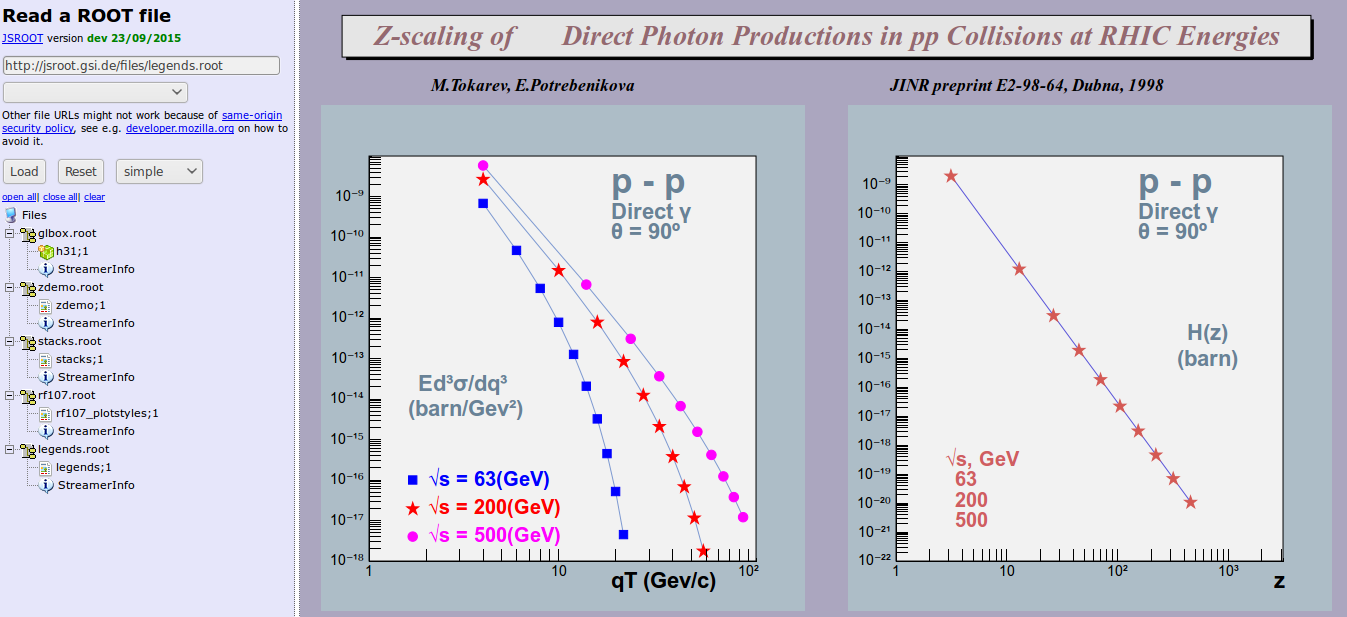
\includegraphics[width=0.8\textwidth]{img/JsROOT}

\end{centering}

\protect\caption{JsROOT example\label{fig:JsROOT-example}}
\end{figure}


In terms of improvements and bugs, after receiving some external feedback
from the DPM team, there is already a number of issues opened on the
DPMbox repository (\href{https://github.com/calvellido/DPMbox/issues}{https://github.com/calvellido/DPMbox/issues}).
The list of things to be addressed includes: 
\begin{itemize}
\item Renaming, for files and collections. For files, this should be feasible
through a \code{MOVE} into the same location. 
\item Show extended information about a collection.
\item Offer more information about the files. Also giving the possibility
to show that information on the right panel, like it happens for collections.
\item Implement a better system for uploads, and also for downloads. Sort
of an upload/download manager including, for example, a progress bar.
\item Improve the error message pop-ups to the final user, trying to show
more information or being less technical.
\item Give the user some configuration options (as sizes or data fields),
going towards a more customizable interface.
\item Show the \code{lcgdm-dav} package version that the system is using.
This is something already implemented in the old interface and it
could be very useful for systems maintenance and testing.
\item Add a huge directory alert. In the DPM network some directories might
contain an enormously number of files (up to hundreds of thousands),
so it would be good to warn the user before opening a collection like
this. 
\end{itemize}
And also, though not being something particularly necessary for DPM,
it would be interesting to:
\begin{itemize}
\item Implement versioning and locks support. Offer the possibility to access
files versions or even revert to a previous version, and delete them.
It could be a good addition the possibility to see which file is locked
for editing by other users. 
\item Add the functionality to drag \& drop a file from your local file
system. With latest HTML5 standards and browser features this shouldn't
be something complicated to implement.
\end{itemize}

\chapter{Acknowledgements\label{chap:Acknowledgements}}

First of all, this work couldn't exist without free software and the
free software community. I am thankful for the contributors who dedicate
their time and efforts to enable people from around the world to use,
study, share and improve free software. Cheers for all the advocates
out there that still think we can make the world a better place through
this.

I want to say thanks to all the people involved at CUSL, for their
work and and the efforts dedicated to maintain such an interesting
initiative through all these years. I also want to say thanks to the
CERN IT-SDC-ID section and the DPM team for the help and the feedback.

I want to thank my supervisors, Manuel Palomo Duarte and Alejandro
Álvarez Ayllón, for helping and advising me all this time, and for
giving me this unforgettable opportunity to contribute to global knowledge
(even if it is with this very minimal and humble contribution).

And last but foremost: 

\emph{Gracias, a mis padres en particular, porque por ellos he llegado hasta
aquí, y a mi familia en general, por apoyarme siempre en la persecución
de mis sueños. }

\appendix


\chapter{Installation manual\label{chap:Installation-manual}}

Installation instructions and some recommendations to set a Disk Pool
Manager instance are listed below.


\section{DPM installation}


\subsection{Installing Scientific Linux 6 }

Image: \href{file:http://linuxsoft.cern.ch/cern/slc6X/iso/SLC_6.6_x86_64_dvd.iso}{linuxsoft.cern.ch/cern/slc6X/iso/SLC\_{}6.6\_{}x86\_{}64\_{}dvd.iso}
\begin{itemize}
\item Install new system
\item Follow the installer instructions
\item Choose \emph{Basic Server / Customize Later}
\item Wait ⌚
\item Reboot, then the system will be updated
\item Please wait again ⌚
\item It's a good idea to redirect local port 2222 to the port 22 of the
virtual machine (so you get SSH connection)
\end{itemize}

\subsection{Installing DPM manually}

DPMbox is already on repositories (please check its status as of September
2015 in~\prettyref{fig:lcgdm-dav_status}), just in case you want
to use the latest version of the packages at the moment you can add
the continuous build repository.


\subsubsection{Repository}
\begin{verbatim}
wget http://svn.cern.ch/guest/lcgdm/extras/build/repos/lcgdm-cbuilds-el6.repo
-P /etc/yum.repos.d
\end{verbatim}

\subsubsection{Install DPM}

Packages
\begin{verbatim}
yum install lcgdm-dav-server dmlite-plugins-adapter dpm-server-mysql
dpm-name-server-mysql dpm
\end{verbatim}

\subsubsection{Install MySQL}
\begin{verbatim}
yum install mysql-server
chkconfig mysqld on
service mysqld start
\end{verbatim}

\subsubsection{Create the tables and the user}
\begin{verbatim}
mysql < /usr/share/lcgdm/create_dpns_tables_mysql.sql 
mysql < /usr/share/lcgdm/create_dpm_tables_mysql.sql 
mysql 
	grant all on cns_db.* to dpmmgr@localhost identified by 'dpmmgr';
	grant all on dpm_db.* to dpmmgr@localhost identified by 'dpmmgr';
\end{verbatim}

\subsubsection{Generate a grid security certificate}
\begin{verbatim}
cd /etc/grid-security
openssl genrsa -out hostkey.pem 1024 
chmod 0400 hostkey.pem
openssl req -new -key hostkey.pem -out hostreq.csr -subj "/DC=es/CN=`hostname -f`" 
openssl x509 -req -days 365 -in hostreq.csr -signkey hostkey.pem -out hostcert.pem 
mkdir dpmmgr
cp hostkey.pem dpmmgr/dpmkey.pem 
cp hostcert.pem dpmmgr/dpmcert.pem 
chown dpmmgr.dpmmgr dpmmgr/*
\end{verbatim}

\subsubsection{Trust this new certificate as CA}
\begin{verbatim}
mkdir /etc/grid-security/certificates 
cd /etc/grid-security/certificates 
cp ../hostcert.pem myca.pem 
ln -s myca.pem $( openssl x509 -hash -noout -in myca.pem )".0"
\end{verbatim}

\subsubsection{Trick the DNS tables}

In /etc/hosts, add your host and host.domain to the end of the list
for 127.0.0.1 y ::1


\subsubsection{Configure DPM y DPNS}

Change /etc/sysconfig/dpm setting this value:
\begin{verbatim}
DPNS_HOST=`hostname` 
\end{verbatim}
Create/etc/NSCONFIG and add:
\begin{verbatim}
dpmmgr/dpmmgr@localhost 
\end{verbatim}
Create/etc/DPMCONFIG and add:
\begin{verbatim}
dpmmgr/dpmmgr@localhost
\end{verbatim}


Then:
\begin{verbatim}
groupadd dpmmgr && useradd -g dpmmgr dpmmgr 
\end{verbatim}
Set in /etc/shift.conf: 
\begin{verbatim}
DPM TRUST host.domain
DPNS TRUST host.domain
RFIOD TRUST host.domain
RFIOD WTRUST host.domain
RFIOD RTRUST host.domain
RFIOD XTRUST host.domain
RFIOD FTRUST host.domain

export DPNS_HOST=localhost
export DPM_HOST=localhost - service dpnsdaemon restart - service dpm restart
\end{verbatim}

\subsubsection{Validate}
\begin{verbatim}
dpns-ls
dpm-qryconf
\end{verbatim}
If you see no message at all, everything is ok.


\subsubsection{Load on startup}
\begin{verbatim}
chkconfig dpnsdaemon on 
chkconfig dpm on
\end{verbatim}

\subsubsection{Add a base}

Create directory:
\begin{verbatim}
dpns-mkdir -p /dpm/domain/home/public 
dpns-chmod 0777 /dpm/domain/home/public
\end{verbatim}
Create a place where files can be hosted:
\begin{verbatim}
dpm-addpool --poolname default --def_filesize 100M 
mkdir /storage 
chown dpmmgr.dpmmgr /storage 
dpm-addfs --poolname default --server host.domain --fs /storage/ 
dpm-qryconf
\end{verbatim}

\subsubsection{Configurate DAV}
\begin{verbatim}
cd /etc/httpd/conf/ 
	Modificar httpd.conf 
	User dpmmgr 
	Group dpmmgr 
	Elimina o comenta las líneas 
		LoadModule dav_module modules/mod_dav.so 
		LoadModule dav_fs_module modules/mod_dav_fs.so 
cd /etc/httpd/conf.d/ 
	rm -f ssl.conf welcome.conf zgridsite.conf 
	En zlcgdm-dav.conf 
		SSLVerifyClient require => SSLVerifyClient optional 
		NSSecureRedirect Off 
		Añade Write to DiskFlags y NSFlags 
		NSRedirectPort 8080 4443 (puertos expuestos al exterior) service httpd restart
\end{verbatim}
Configure the firewall to ports 443 and 80 and that should be all. 

If you are setting this machine on a virtual system, add a redirection
from 443 to 4443 and from 80 a 8080, also you can relax the security
directives disabling the firewall:
\begin{verbatim}
service iptables stop / chkconfig iptables off
\end{verbatim}
Or deactivating selinux:
\begin{verbatim}
setenforce 0 
vim /etc/selinux/config SELINUX=permissive
\end{verbatim}
From an external machine accessing \code{https://localhost:8080/dpm/}
something should appear now. 


\section{DPMbox installation}

DPMbox it's included on build 0.16.0-1 of \code{lcgdm-dav}, on RPM
repositories, as of September 2015 it is on testing channel for EPEL
5, 6, 7 and on stable for Fedora 22 and 23. This can be checked on~\prettyref{fig:lcgdm-dav_status} 

This update can be installed with the \textquotedbl{}yum\textquotedbl{}
update program. Use su -c '\code{yum update lcgdm-dav}' at the command
line. For more information, refer to \textquotedbl{}Managing Software
with yum\textquotedbl{}, available at \href{http://docs.fedoraproject.org/yum/}{http://docs.fedoraproject.org/yum/}


\chapter{Developer manual\label{chap:Developer-manual}}


\section{DPM server environment}

It's recommended to test DPMbox against a proper DPM machine. You
can install a DPM instance following the guide above:~\nameref{chap:Installation-manual}.

When installed DPMbox files will be located on the path:
\begin{verbatim}
/usr/share/lcgdm-dav/lcgdm-dav/DPMbox/
\end{verbatim}


Also you can download last DPMbox version from its code repository
address~\cite{11_valencia_calvellido_2015}. Be aware that you should
not touch the server and root parameters in the config.js file as
they will be obtained automatically from the location (those lines
on config.js will be already set). 


\section{WebDAV server environment}

You may encounter problems setting an instance of DPM running. In
that case you can still dig into DPMbox by testing it on a WebDAV
server. You only need an Apache server and a couple of modules.

Follow your system recommendations to install Apache server. The WebDAV
modules \code{mod\_dav} and \code{mod\_dav\_fs} are bundled with
any version of Apache ≥ 2.0~\cite{apache_mod_dav}~\cite{apache_mod_dav_fs},
so enable them, and then indicate Apache where the WebDAV filesystem
will be hosted on your system. 

These operations could vary from system to system, but the following
are guide steps to install a WebDAV server on a Linux Debian based
system~\cite{install_webdav}. For other OS some instructions will
be very similar, even identical:


\subsection{Install Apache}

Our implementation of WebDAV will be established on Apache through
the use of the WebDAV module.

First, you will need to install Apache from Ubuntu's default repositories.
\begin{verbatim}
sudo apt-get update
sudo apt-get install apache2
\end{verbatim}


You now have a fully functioning web server installed. It should be
accessible already by navigating to your server's IP address in a
web browser. 


\subsection{Enable WebDAV}

Apache has built-in support for WebDAV with a few modules. We simply
have to enable them to get access to their functions.

Enable the WebDAV modules with the following two commands:
\begin{verbatim}
sudo a2enmod dav
sudo a2enmod dav_fs
\end{verbatim}


We now need to restart the server to implement the changes:
\begin{verbatim}
sudo service apache2 restart
\end{verbatim}


WebDAV as a functionality is now enabled, but we still haven't configured
it correctly yet for our server. 


\subsection{Create the FileSystem}

We will create a directory that will house our WebDAV file content.

The default document root of the Apache server on Ubuntu is located
at \code{/var/www}. However, we will be creating an alias, which
will allow us to keep our directory content elsewhere.

In this guide, we will place our WebDAV content at \code{/webdav/}
\begin{verbatim}
sudo mkdir /webdav
\end{verbatim}


Give the web user, which is \code{www-data}, ownership of the new
directory, so that it can serve content correctly:
\begin{verbatim}
sudo chown www-data /webdav
\end{verbatim}

\subsection{Set Up Password Protection}

We can create an authentication procedure for accessing the directory
content by creating an htpasswd file.

We will place it outside of the content directory so that it will
not be accessible to users of our system. Create a username within
the command call and you will be prompted for an associated password:
\begin{verbatim}
sudo htpasswd -c /etc/apache2/webdav.password username
\end{verbatim}


Right now, anybody can view the username and hashed password in the
file. We will assign group ownership of the file to www-data and then
lock down the permissions for everyone else:
\begin{verbatim}
sudo chown root:www-data /etc/apache2/webdav.password 
sudo chmod 640 /etc/apache2/webdav.password
\end{verbatim}

\subsection{Configure Apache}

Now, we will have to configure access to our content directory and
tell Apache to use the WebDAV modules to serve that location. We will
also have to note the authentication scheme we've created.

Edit the main virtual host configuration with root privileges:
\begin{verbatim}
sudo nano /etc/apache2/sites-available/default
\end{verbatim}


Here, our web content is served out of /var/www like normal. We will
add some information that will allow Apache to treat content in our
new directory as WebDAV material.

Below the directory listings, we will add an alias directive to tell
Apache that requests for \textquotedbl{}/webdav\textquotedbl{} should
be served out of the /webdav directory we created.

We will then add options to allow authentication using the methods
we established.
\begin{verbatim}
. . . 
. . . 
<Directory /var/www/> 
	Options Indexes FollowSymLinks MultiViews 
	AllowOverride None 
	Order allow,deny 
	allow from all 
</Directory>

Alias /webdav /webdav

<Location /webdav> 
	Options Indexes 
	DAV On AuthType Basic AuthName "webdav" 
	AuthUserFile /etc/apache2/webdav.password 
	Require valid-user 
</Location>
. . . 
. . .
\end{verbatim}


Save and close the file.

Restart Apache with the following command:
\begin{verbatim}
sudo service apache2 restart
\end{verbatim}

\subsection{Test the Results}

You can test the results of you configuration first in a web browser,
and then in a WebDAV client. 


\subsubsection{Web Browser Test}

To test that your authentication is working correctly, navigate to
your server's IP address or domain name using a web browser.

You should see the default Apache index.html file:

\begin{figure}
\begin{center}


\includegraphics{img/ApacheItWorks}

\end{center}

\protect\caption{Apache default index file}
\end{figure}


This demonstrates that the regular web functionality is working.

Now, navigate to your IP address or domain name followed by \textquotedbl{}/webdav\textquotedbl{}:
\begin{verbatim}
your_IP_address_or_domain/webdav
\end{verbatim}


You should be prompted for the username and password combination you
set up earlier. Afterwards, you should see an empty directory listing:

\begin{figure}
\begin{center}

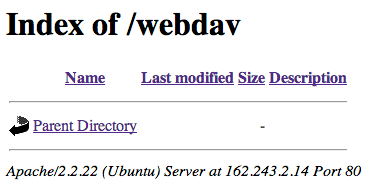
\includegraphics{img/EmptyWebDAV}

\end{center}

\protect\caption{Empty WebDAV}
\end{figure}


We don't currently have any content here, but we'll be able to change
that by accessing the same area with a WebDAV client. 


\subsubsection{WebDAV Client Test}

There are many WebDAV clients and support for WebDAV access is baked
into many popular file managers.

For simplicity's sake, we'll use an easy command-line WebDAV client
called \textquotedbl{}cadaver\textquotedbl{} in this guide.

Preferably from another droplet or Linux machine, install cadaver
from the default repositories:
\begin{verbatim}
sudo apt-get install cadaver
\end{verbatim}


Now, let's create a file that we'll upload to the WebDAV directory:
\begin{verbatim}
cd ~ 
touch testfile
\end{verbatim}


Next, we'll connect using the same location we used to access from
the browser:
\begin{verbatim}
cadaver http://your_IP_address_or_domain/webdav

Authentication required for webdav on server `162.243.2.14': 
Username:
\end{verbatim}


You must type the \textquotedbl{}http://\textquotedbl{} portion for
cadaver to find your server correctly. We will need to authenticate
again, and then we'll be dropped into a command-line interface.
\begin{verbatim}
dav:/webdav/>
\end{verbatim}


From here, we can operate the client and host at the same time using
commands that are similar to regular Linux commands.

To list the contents of the server directory, type:
\begin{verbatim}
ls

Listing collection `/webdav/': collection is empty.
\end{verbatim}


The directory is empty. Let's change that uploading our test file:
\begin{verbatim}
put testfile
\end{verbatim}


We can try the list command again and see the file is now on the server:
\begin{verbatim}
ls

Listing collection `/webdav/': succeeded. 
	testfile 0 Sep 20 19:36
\end{verbatim}


We can make a directory and change into it by typing:
\begin{verbatim}
mkdir hello 
cd hello
\end{verbatim}


We can then create a file by typing:
\begin{verbatim}
edit file.html
\end{verbatim}


We can insert whatever content we want:
\begin{verbatim}
<h1>Hi!!!</h1>
\end{verbatim}


When we are finished, we can type exit to close the connection:
\begin{verbatim}
exit
\end{verbatim}


Now, if we go back to our web browser, the changes that we've made
are visible:
\begin{verbatim}
your_IP_address_or_domain/webdav
\end{verbatim}
\begin{figure}
\begin{center}

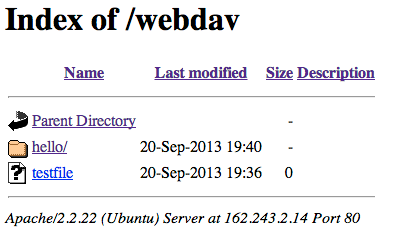
\includegraphics{img/WebDAV_content}

\end{center}

\protect\caption{WebDAV content}
\end{figure}



\subsection{Conclusion}

You should now have a WebDAV directory complete with basic authentication.
If your directory contains content that absolutely must be kept secure,
you might want to implement an SSL solution on top of the password
authentication. 

Many file managers and clients exist that can seamlessly access and
modify WebDAV content as if it were additional local storage. WebDAV
allows for a much more dynamic HTTP experience than is traditionally
possible.


\subsection{DPMbox integration}

You can download last DPMbox version from its code repository address~\cite{11_valencia_calvellido_2015}. 

To use it on an Apache environment, extract the DPMbox distribution
on your server and access through your browser to the existing index.html.
Before testing on your local context, or if you are using DPMbox to
connect to an external DPM server, please assign the values on config.js
file properly. 

The server value must be filled with something like 'http://lxfsra04a04.cern.ch'
or 'localhost' and the root parameter (the directory at where the
interface will start to read WebDAV content) should be set to anything
like '/dpm/cern.ch/home/dteam/aalvarez/public/' or '/webdav/' (trailing
backslash needed).


\subsection{Cross-Origin Resource Sharing (CORS) policy}

If you are testing DPMbox with a WebDAV server located beyond your
own machine, please read this section carefully to make DPMbox work
properly.

In the DPM architecture one entity handles the namespace with the
metadata, and other ones store the files with the actual data. This
means that any request must go through a server hosting the namespace
first, and then redirect to the disk node storing the physical file.
We execute a PUT call and the file won’t be yet uploaded but DPM will
answer back, then our web application has to try a second time. The
URL needed to actually do the PUT would look like this, you can see
the specific DPM node where the file will be uploaded, including a
token validating the transaction:
\begin{verbatim}
http://lxfsra04a04.cern.ch/srv/dpm/01/nogroup/2015-03-02/XHR.js.zip.2900489
.0?sfn=%2Fdpm%2Fcern.ch%2Fhome%2Fdteam%2Faalvarez%2Fpublic%2Fcollection_d
%2FXHR.js.zip&dpmtoken=dbf5fcbe-7c31-4849-aa57-b07c6b474f5e&token=ojkU%2
FdgyPqTYEvu4TfZAyueVDqQ%3D%401425288602%401
\end{verbatim}
User agents commonly apply same-origin restrictions to network requests.
These restrictions prevent a client-side Web application as DPMbox
running from one origin from obtaining data retrieved from another
origin, and also limit unsafe HTTP requests that can be automatically
launched toward destinations that differ from the running application’s
origin. In user agents that follow this pattern, network requests
typically include user credentials with cross-origin requests, including
HTTP authentication and cookie information. As DPMbox relies heavily
on XHR calls this has to be handled carefully or you’ll face a lot
of error messages like this:
\begin{verbatim}
Cross-Origin Request Blocked: The Same Origin Policy disallows reading the 
remote resource at http://lxfsra04a04.cern.ch/dpm/cern.ch/home/dteam/aalvarez/
public/test5.file. (Reason: CORS header 'Access-Control-Allow-Origin' missing).
\end{verbatim}
You can check a bit of history of XHR and CORS and why this is happening
on~\cite{1_cruz_2015}.

The CORS headers response configuration for an Apache WebDAV server
that gets connections from DPMbox must look like~\prettyref{lis:CORSconfig}.
\begin{verse}
\begin{lstlisting}[caption={Access-Control Configuration},label={lis:CORSconfig},float,basicstyle={\footnotesize\ttfamily},columns=fullflexible]
Access-Control-Allow-Origin: UrlWhereDPMboxIsHosted.host 
Access-Control-Allow-Credentials: true 
Access-Control-Allow-Methods: ACL, CANCELUPLOAD, CHECKIN, CHECKOUT, COPY, DELETE, GET, HEAD, LOCK, MKCALENDAR, MKCOL, MOVE, OPTIONS, POST, PROPFIND, PROPPATCH, PUT, REPORT, SEARCH, UNCHECKOUT, UNLOCK, UPDATE, VERSION-CONTROL 
Access-Control-Allow-Headers: Authorization, Overwrite, Destination, Content-Type, Depth, User-Agent, Translate, Range, Content-Range, Timeout, X-File-Size, X-Requested-With, Accept, Accept-Version, If-Modified-Since, X-File-Name, Cache-Control, Location, Lock-Token, If, X-No-Redirect 
Access-Control-Expose-Headers: DAV, content-length, Allow, Location
\end{lstlisting}

\end{verse}

\section{Extending DPMbox}

Once the DPM or WebDAV server is up and running you can start playing
with DPMbox. As you have seen DPMbox works basically through three
files: 
\begin{description}
\item [{dpmbox-ui.js}] User interface code
\item [{jquery.dpm.js}] Server interaction code
\item [{jquery.dpmFilters.js}] Filters to adapt the server response information 
\end{description}


You can find more information about the content and organization of
these files in the section \nameref{sec:System-design}. 

Be careful when changing the context if you are developing on local
and deploying over some external server. Also, as the interface is
based on an external library, please read its documentation and follow
its developer recommendations and advices~\cite{8_w2ui_2015}.

And you are all set, happy coding!


\chapter{User manual\label{chap:User-manual}}

\renewcommand{\textflush}{flushepinormal}\setlength\epigraphwidth{.6\textwidth}\setlength\afterepigraphskip{2\baselineskip}\setlength{\epigraphrule}{0pt}\epigraphhead[40]{\epigraph{\emph{``Any product that needs a manual to work is broken.''}}{--- Elon Musk, \emph{founder of Paypal, SpaceX or Tesla}~\cite{1_musk_2015}}}

Based on the words of Elon Musk, one of the main design goals in DPMbox
was to make this user manual unnecessary. Even so, here it is in case
someone thinks DPMbox is \emph{broken}.


\section{Introduction}

The Disk Pool Manager (DPM) is a lightweight grid storage component,
allowing access to data using commonly used grid protocols. DPMbox
is its new web-based interface developed in JavaScript. Its look and
feel is similar to desktop file explorers, so you won’t spend lots
of time to adapt to its behaviour.

You can perform various operations with application data including
(multiple) file upload, (multiple) file download, (multiple) delete
of files and collections. Besides that you can also perform searches
based on various file properties inside a directory and sort the content
by those same properties.

Its panels are slightly responsive for a fast adjustment to your screen,
and besides that, it has a flexible layout, that you can adapt to
suit your needs.

An overview of the main interface is attached, please check~\prettyref{fig:dpmbox_functionality}.


\section{Functionality}

DPMbox functionality include:
\begin{itemize}
\item Collections exploring and navigation
\item Collections creation and deletion
\item Files download, including massive download
\item Files upload, including massive upload
\item Files removing
\item Filter and/or order the content inside a collection
\item Search inside a collection
\item Get metalinks
\end{itemize}
\begin{figure}[H]
\label{fig:dpmbox_functionality}

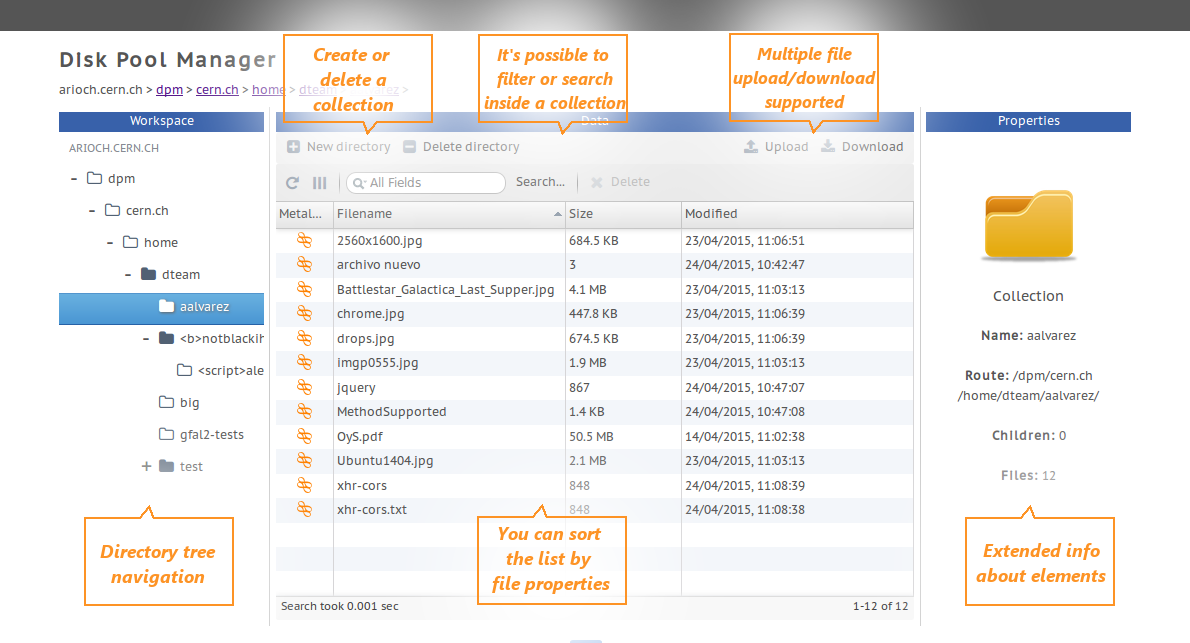
\includegraphics[width=1\textwidth]{img/DPMbox-screenshot_comments}

\protect\caption{DPMbox main functionality}
\end{figure}



\section{Requirements}

In order to use DPMbox on your system, the DPM server must be updated
to at least \code{lcgdm-dav} version 0.16. If you are unsure about
this, please ask your Disk Pool Manager administrator about this.

Besides that, the requirements are reduced to the web browser version
you are using. It's strictly recommended that you use an updated browser,
specifically DPMbox will work on (not restricted to):
\begin{itemize}
\item Google Chrome/Chromium, any version higher than v17
\item Mozilla Firefox, starting on version 7
\item Apple Safari, a more recent version than release 5
\item Microsoft Internet Explorer, version 9 onwards
\end{itemize}

\section{How to use DPMbox}

Just write the location of the DPM server that you would like to access.
If the server is already updated you will be presented in your browser
with a brand new interface that will look like the one in figure~\ref{fig:dpmbox_functionality}.

If, for any reason, you have problems using DPMbox a switchback link
has been added to get back to the old and plain WebDAV interface.
It will be located on the left down corner of your browser, a small
caption of text like in~\ref{fig:oldinterface_link}. Every other
new access will remember your interface choice (if you have cookies
activated on your browser), though you can at any time change again
to DPMbox and viceversa.

\begin{figure}[H]
\begin{centering}

\label{fig:oldinterface_link}


\includegraphics{img/howtouse_2}

\end{centering}\protect\caption{How to use - Old interface link}
\end{figure}


A folder icon on the left panel set on white indicates that the directory
hasn't been yet read, so it could have more children or not. Clicking
on the directory name will read the collection information from the
server, presenting you the files contained on the center panel, and
expanding the directory tree if there are children inside that route.
When a directory is read, a + or a − icon are added to the left of
the collection name, by them you can expand and collapse the tree
hanging from that node.

Yoy can see a visual representation of the main functionalities in
the figures attached: navigation~\ref{fig:howto-navigation}, files
uploading~\ref{fig:howto-uploading}, create and delete collections~\ref{fig:howto-collections},
filtering and searching~\ref{fig:howto-searching} and sorting~\ref{fig:howto-sorting}.

\clearpage

\begin{figure}[H]
\label{fig:howto-navigation}

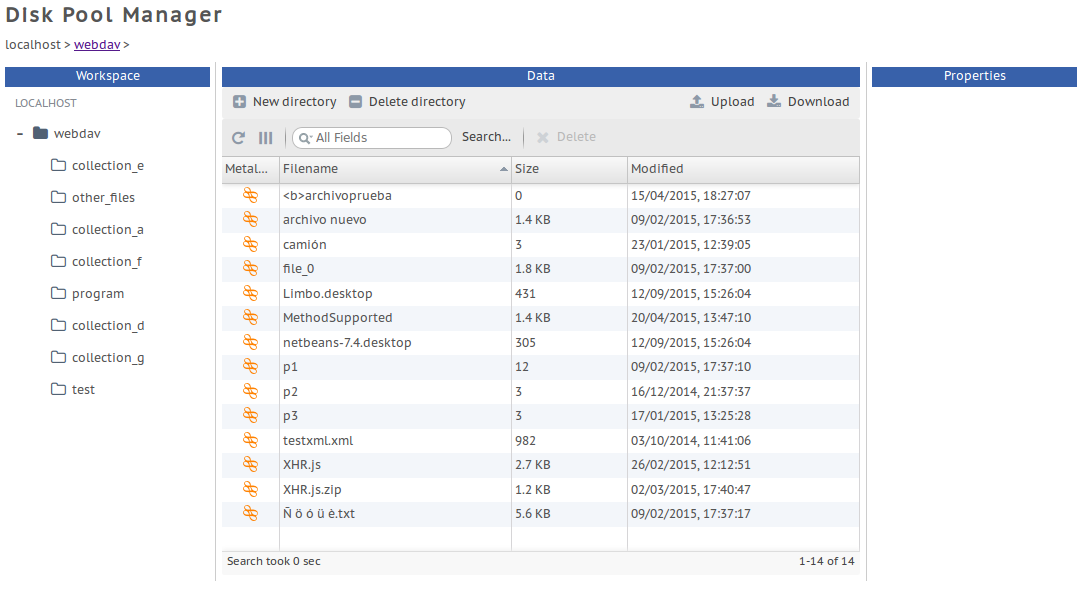
\includegraphics[width=0.5\textwidth]{img/howtouse_1}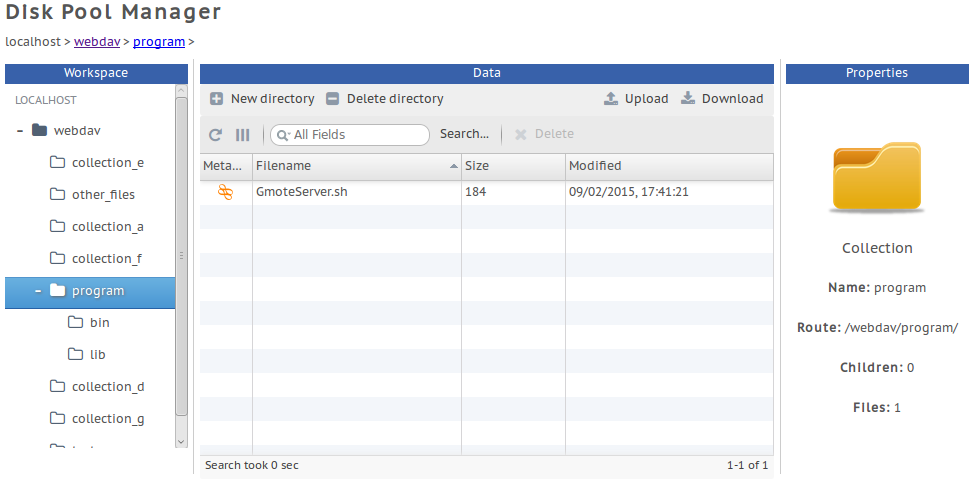
\includegraphics[width=0.5\textwidth]{img/howtouse_3}

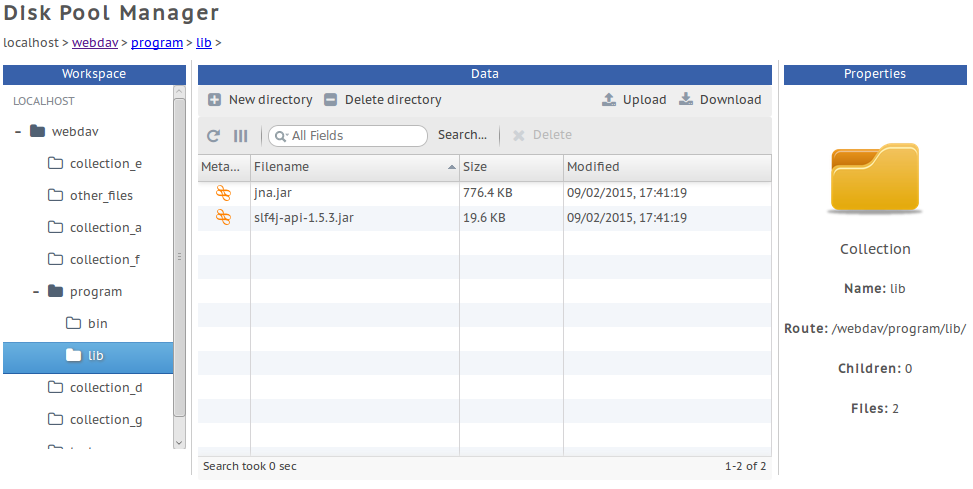
\includegraphics[width=0.5\textwidth]{img/howtouse_4}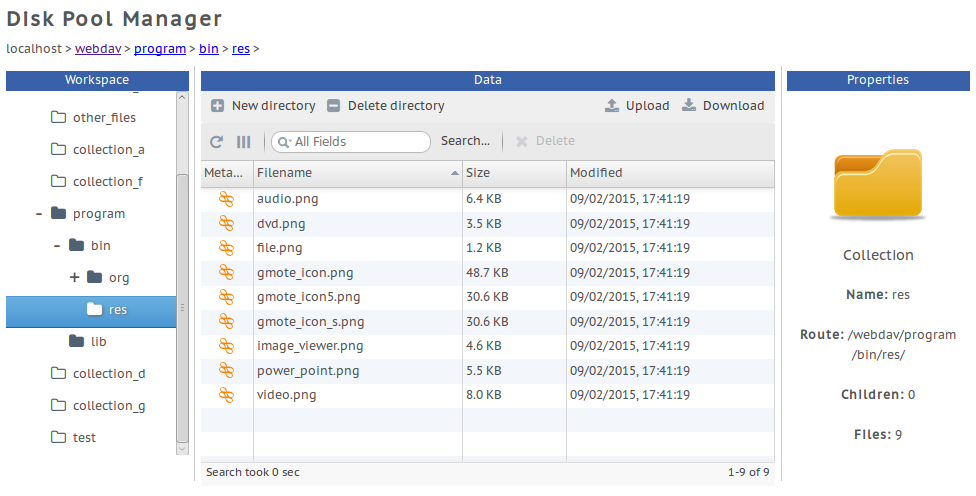
\includegraphics[width=0.5\textwidth]{img/howtouse_5}

\protect\caption{How to use - Navigation}
\end{figure}


\begin{figure}[H]
\label{fig:howto-uploading}

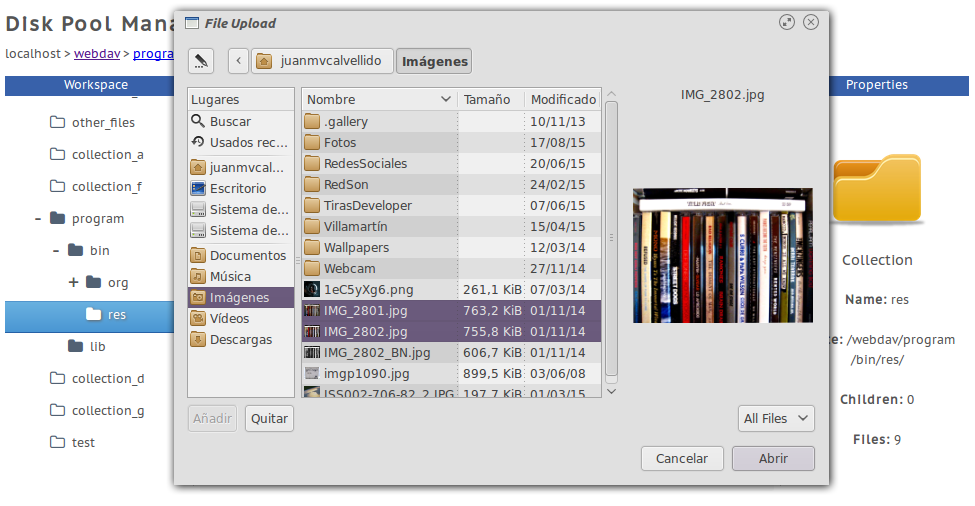
\includegraphics[width=0.5\textwidth]{img/howtouse_6}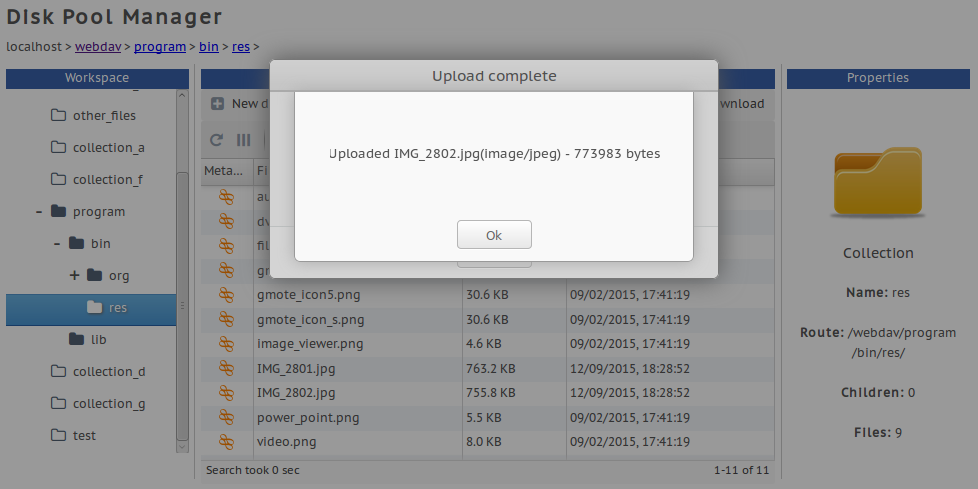
\includegraphics[width=0.5\textwidth]{img/howtouse_7}

\protect\caption{How to use - Uploading}
\end{figure}


\begin{figure}[H]
\label{fig:howto-collections}

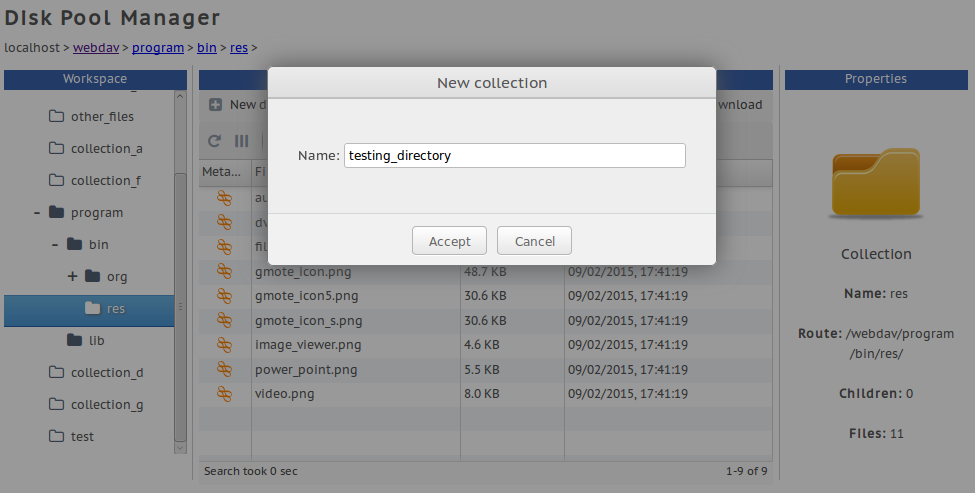
\includegraphics[width=0.5\textwidth]{img/howtouse_11}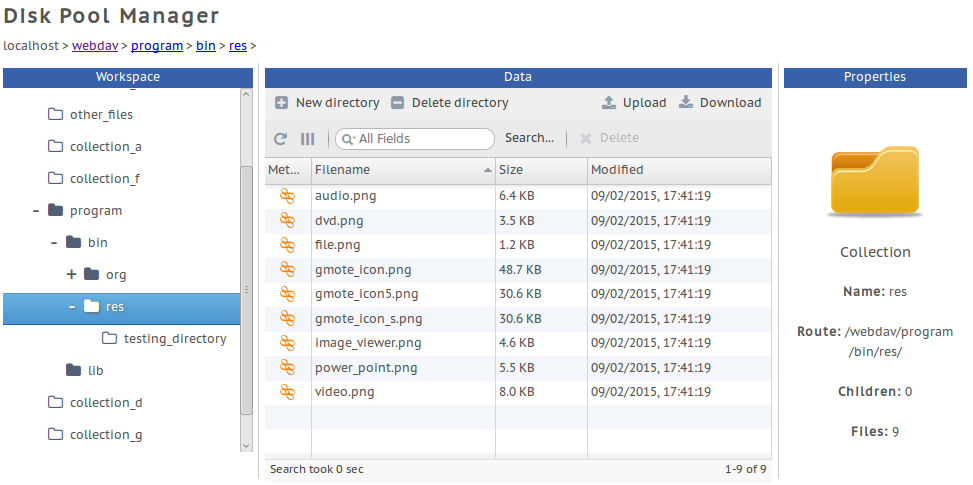
\includegraphics[width=0.5\textwidth]{img/howtouse_12}

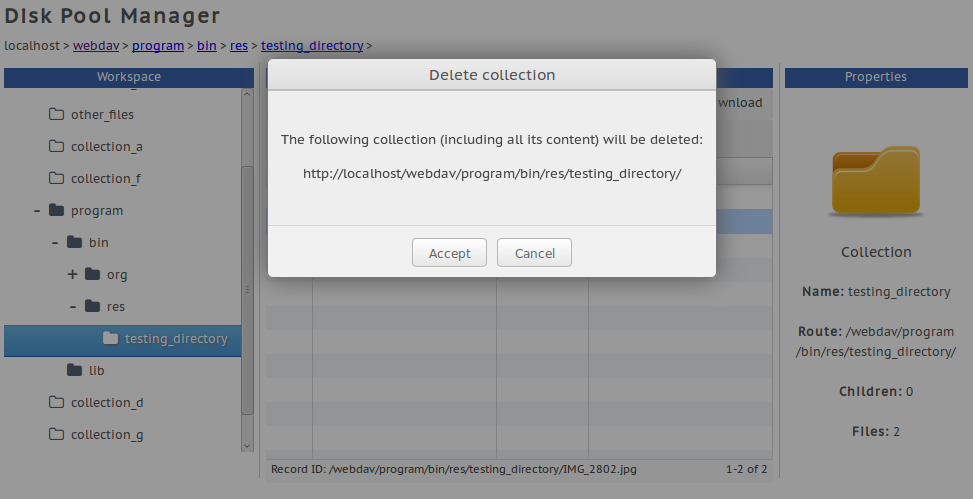
\includegraphics[width=0.5\textwidth]{img/howtouse_13}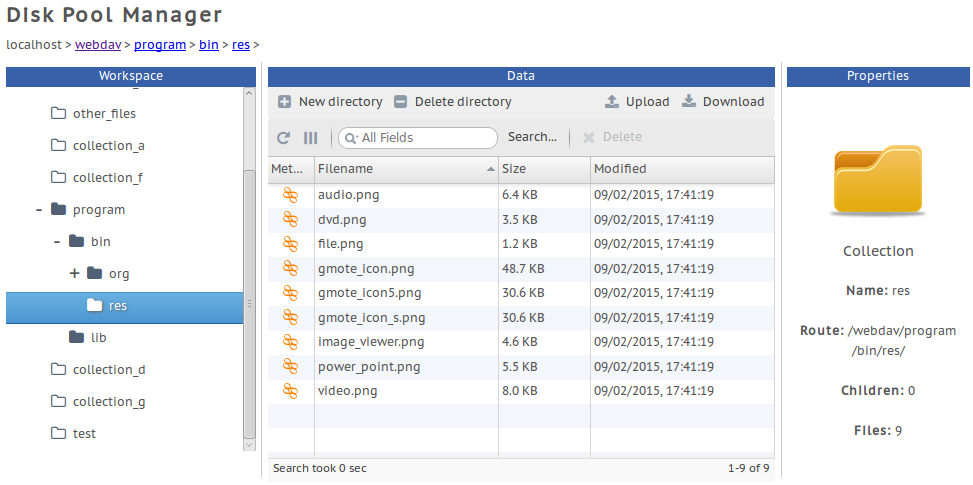
\includegraphics[width=0.5\textwidth]{img/howtouse_14}

\protect\caption{How to use - Create and delete collection}
\end{figure}


\begin{figure}[H]
\label{fig:howto-searching}

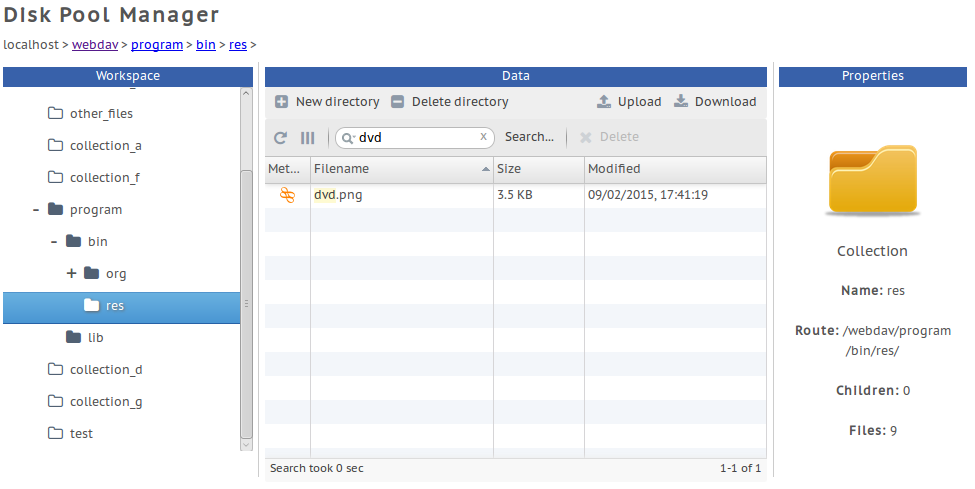
\includegraphics[width=0.5\textwidth]{img/howtouse_15}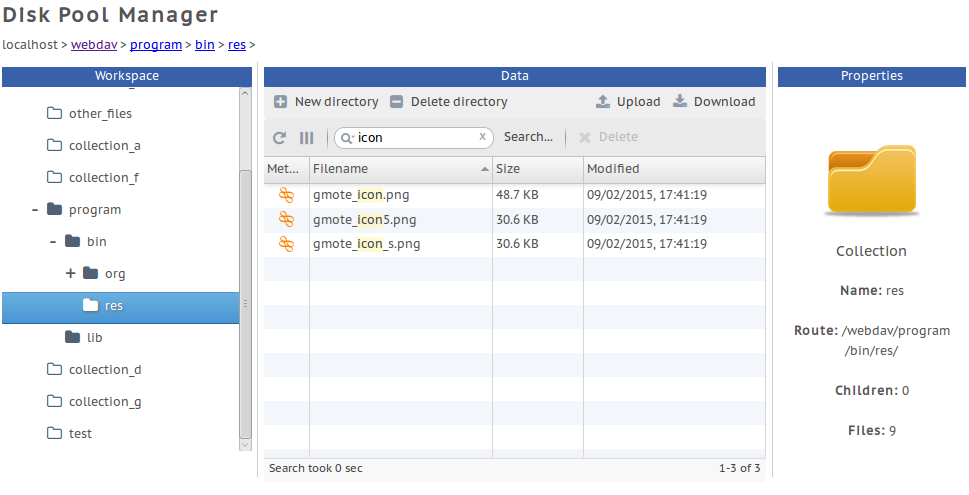
\includegraphics[width=0.5\textwidth]{img/howtouse_16}

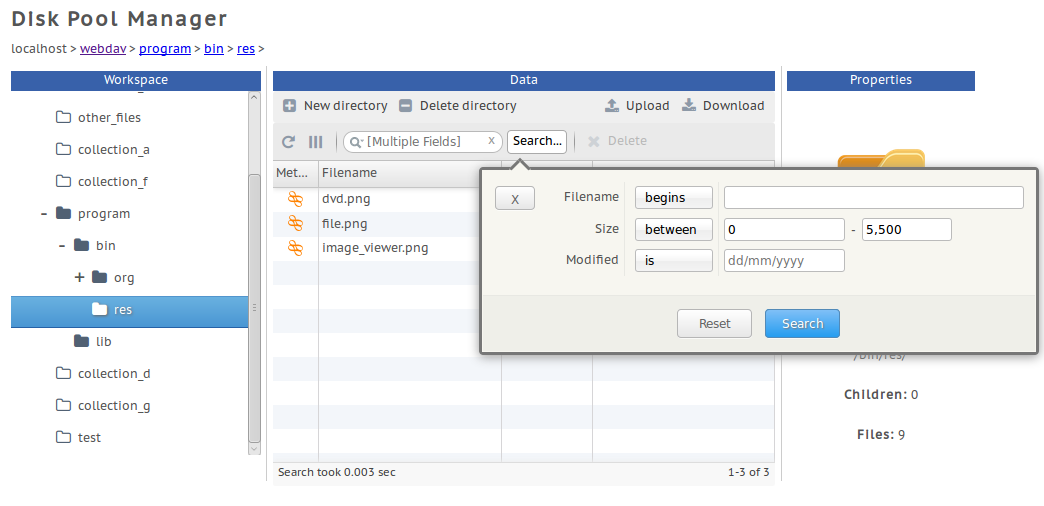
\includegraphics[width=0.5\textwidth]{img/howtouse_17}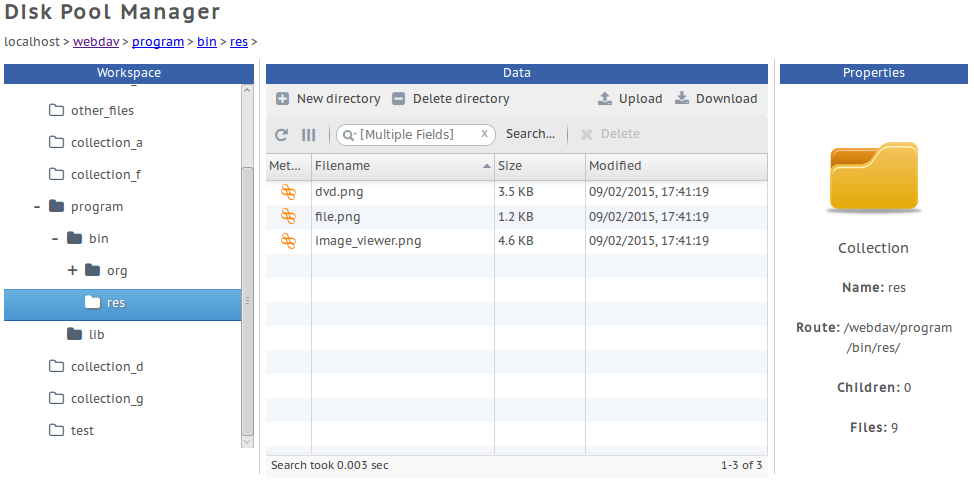
\includegraphics[width=0.5\textwidth]{img/howtouse_18}

\protect\caption{How to use - Filtering and searching}
\end{figure}


\begin{figure}[H]
\label{fig:howto-sorting}

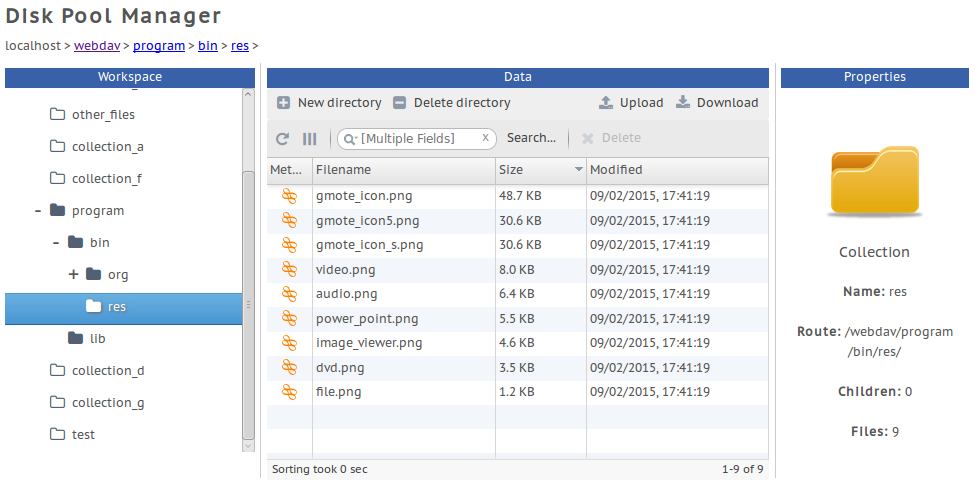
\includegraphics[width=0.5\textwidth]{img/howtouse_19}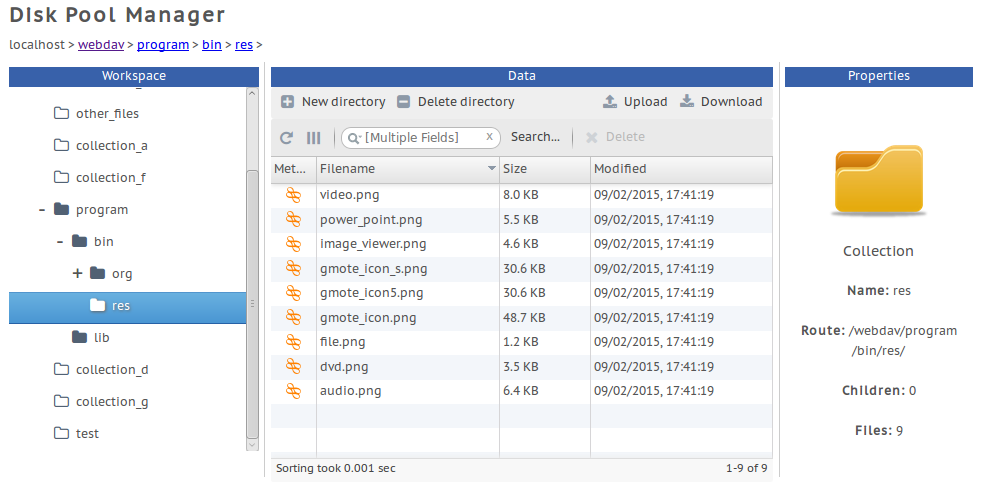
\includegraphics[width=0.5\textwidth]{img/howtouse_20}

\protect\caption{How to use - Sorting}
\end{figure}


\bibliographystyle{splncs03}
\bibliography{references}



\addchap{GNU Free Documentation License\label{chap:GNU-Free-Documentation}}

\begin{center}
       Version 1.3, 3 November 2008
 
Copyright \copyright{} 2000, 2001, 2002, 2007, 2008  Free Software Foundation, Inc.

  \bigskip\texttt{<http://fsf.org/>}\bigskip

Everyone is permitted to copy and distribute verbatim copies  of this license document, but changing it is not allowed. \end{center}
\begin{center} {\bf\large Preamble} \end{center}
The purpose of this License is to make a manual, textbook, or other functional and useful document ``free'' in the sense of freedom: to assure everyone the effective freedom to copy and redistribute it, with or without modifying it, either commercially or noncommercially. Secondarily, this License preserves for the author and publisher a way to get credit for their work, while not being considered responsible for modifications made by others.

This License is a kind of ``copyleft'', which means that derivative works of the document must themselves be free in the same sense.  It complements the GNU General Public License, which is a copyleft license designed for free software.

We have designed this License in order to use it for manuals for free software, because free software needs free documentation: a free program should come with manuals providing the same freedoms that the software does.  But this License is not limited to software manuals; it can be used for any textual work, regardless of subject matter or whether it is published as a printed book.  We recommend this License principally for works whose purpose is instruction or reference.
\begin{center} {\Large\bf 1. APPLICABILITY AND DEFINITIONS\par} \phantomsection \addcontentsline{toc}{section}{1. APPLICABILITY AND DEFINITIONS} \end{center}
This License applies to any manual or other work, in any medium, that contains a notice placed by the copyright holder saying it can be distributed under the terms of this License.  Such a notice grants a world-wide, royalty-free license, unlimited in duration, to use that work under the conditions stated herein.  The ``\textbf{Document}'', below, refers to any such manual or work.  Any member of the public is a licensee, and is addressed as ``\textbf{you}''.  You accept the license if you copy, modify or distribute the work in a way requiring permission under copyright law.

A ``\textbf{Modified Version}'' of the Document means any work containing the Document or a portion of it, either copied verbatim, or with modifications and/or translated into another language.

A ``\textbf{Secondary Section}'' is a named appendix or a front-matter section of the Document that deals exclusively with the relationship of the publishers or authors of the Document to the Document's overall subject (or to related matters) and contains nothing that could fall directly within that overall subject.  (Thus, if the Document is in part a textbook of mathematics, a Secondary Section may not explain any mathematics.)  The relationship could be a matter of historical connection with the subject or with related matters, or of legal, commercial, philosophical, ethical or political position regarding them.

The ``\textbf{Invariant Sections}'' are certain Secondary Sections whose titles are designated, as being those of Invariant Sections, in the notice that says that the Document is released under this License.  If a section does not fit the above definition of Secondary then it is not allowed to be designated as Invariant.  The Document may contain zero Invariant Sections.  If the Document does not identify any Invariant Sections then there are none.

The ``\textbf{Cover Texts}'' are certain short passages of text that are listed, as Front-Cover Texts or Back-Cover Texts, in the notice that says that the Document is released under this License.  A Front-Cover Text may be at most 5 words, and a Back-Cover Text may be at most 25 words.

A ``\textbf{Transparent}'' copy of the Document means a machine-readable copy, represented in a format whose specification is available to the general public, that is suitable for revising the document straightforwardly with generic text editors or (for images composed of pixels) generic paint programs or (for drawings) some widely available drawing editor, and that is suitable for input to text formatters or for automatic translation to a variety of formats suitable for input to text formatters.  A copy made in an otherwise Transparent file format whose markup, or absence of markup, has been arranged to thwart or discourage subsequent modification by readers is not Transparent. An image format is not Transparent if used for any substantial amount of text.  A copy that is not ``Transparent'' is called ``\textbf{Opaque}''.

Examples of suitable formats for Transparent copies include plain ASCII without markup, Texinfo input format, LaTeX input format, SGML or XML using a publicly available DTD, and standard-conforming simple HTML, PostScript or PDF designed for human modification.  Examples of transparent image formats include PNG, XCF and JPG.  Opaque formats include proprietary formats that can be read and edited only by proprietary word processors, SGML or XML for which the DTD and/or processing tools are not generally available, and the machine-generated HTML, PostScript or PDF produced by some word processors for output purposes only.

The ``\textbf{Title Page}'' means, for a printed book, the title page itself, plus such following pages as are needed to hold, legibly, the material this License requires to appear in the title page.  For works in formats which do not have any title page as such, ``Title Page'' means the text near the most prominent appearance of the work's title, preceding the beginning of the body of the text.

The ``\textbf{publisher}'' means any person or entity that distributes copies of the Document to the public.

A section ``\textbf{Entitled XYZ}'' means a named subunit of the Document whose title either is precisely XYZ or contains XYZ in parentheses following text that translates XYZ in another language.  (Here XYZ stands for a specific section name mentioned below, such as ``\textbf{Acknowledgements}'', ``\textbf{Dedications}'', ``\textbf{Endorsements}'', or ``\textbf{History}''.)   To ``\textbf{Preserve the Title}'' of such a section when you modify the Document means that it remains a section ``Entitled XYZ'' according to this definition.

The Document may include Warranty Disclaimers next to the notice which states that this License applies to the Document.  These Warranty Disclaimers are considered to be included by reference in this License, but only as regards disclaiming warranties: any other implication that these Warranty Disclaimers may have is void and has no effect on the meaning of this License.
\begin{center} {\Large\bf 2. VERBATIM COPYING\par} \phantomsection \addcontentsline{toc}{section}{2. VERBATIM COPYING} \end{center}
You may copy and distribute the Document in any medium, either commercially or noncommercially, provided that this License, the copyright notices, and the license notice saying this License applies to the Document are reproduced in all copies, and that you add no other conditions whatsoever to those of this License.  You may not use technical measures to obstruct or control the reading or further copying of the copies you make or distribute.  However, you may accept compensation in exchange for copies.  If you distribute a large enough number of copies you must also follow the conditions in section~3.

You may also lend copies, under the same conditions stated above, and you may publicly display copies.
\begin{center} {\Large\bf 3. COPYING IN QUANTITY\par} \phantomsection \addcontentsline{toc}{section}{3. COPYING IN QUANTITY} \end{center}
If you publish printed copies (or copies in media that commonly have printed covers) of the Document, numbering more than 100, and the Document's license notice requires Cover Texts, you must enclose the copies in covers that carry, clearly and legibly, all these Cover Texts: Front-Cover Texts on the front cover, and Back-Cover Texts on the back cover.  Both covers must also clearly and legibly identify you as the publisher of these copies.  The front cover must present the full title with all words of the title equally prominent and visible.  You may add other material on the covers in addition. Copying with changes limited to the covers, as long as they preserve the title of the Document and satisfy these conditions, can be treated as verbatim copying in other respects.

If the required texts for either cover are too voluminous to fit legibly, you should put the first ones listed (as many as fit reasonably) on the actual cover, and continue the rest onto adjacent pages.

If you publish or distribute Opaque copies of the Document numbering more than 100, you must either include a machine-readable Transparent copy along with each Opaque copy, or state in or with each Opaque copy a computer-network location from which the general network-using public has access to download using public-standard network protocols a complete Transparent copy of the Document, free of added material. If you use the latter option, you must take reasonably prudent steps, when you begin distribution of Opaque copies in quantity, to ensure that this Transparent copy will remain thus accessible at the stated location until at least one year after the last time you distribute an Opaque copy (directly or through your agents or retailers) of that edition to the public.

It is requested, but not required, that you contact the authors of the Document well before redistributing any large number of copies, to give them a chance to provide you with an updated version of the Document.
\begin{center} {\Large\bf 4. MODIFICATIONS\par} \phantomsection \addcontentsline{toc}{section}{4. MODIFICATIONS} \end{center}
You may copy and distribute a Modified Version of the Document under the conditions of sections 2 and 3 above, provided that you release the Modified Version under precisely this License, with the Modified Version filling the role of the Document, thus licensing distribution and modification of the Modified Version to whoever possesses a copy of it.  In addition, you must do these things in the Modified Version:

\begin{itemize} \item[A.]     Use in the Title Page (and on the covers, if any) a title distinct    from that of the Document, and from those of previous versions    (which should, if there were any, be listed in the History section    of the Document).  You may use the same title as a previous version    if the original publisher of that version gives permission.     \item[B.]    List on the Title Page, as authors, one or more persons or entities    responsible for authorship of the modifications in the Modified    Version, together with at least five of the principal authors of the    Document (all of its principal authors, if it has fewer than five),    unless they release you from this requirement.     \item[C.]    State on the Title page the name of the publisher of the    Modified Version, as the publisher.     \item[D.]    Preserve all the copyright notices of the Document.     \item[E.]    Add an appropriate copyright notice for your modifications    adjacent to the other copyright notices.     \item[F.]    Include, immediately after the copyright notices, a license notice    giving the public permission to use the Modified Version under the    terms of this License, in the form shown in the Addendum below.     \item[G.]    Preserve in that license notice the full lists of Invariant Sections    and required Cover Texts given in the Document's license notice.     \item[H.]    Include an unaltered copy of this License.     \item[I.]    Preserve the section Entitled ``History'', Preserve its Title, and add    to it an item stating at least the title, year, new authors, and    publisher of the Modified Version as given on the Title Page.  If    there is no section Entitled ``History'' in the Document, create one    stating the title, year, authors, and publisher of the Document as    given on its Title Page, then add an item describing the Modified    Version as stated in the previous sentence.     \item[J.]    Preserve the network location, if any, given in the Document for    public access to a Transparent copy of the Document, and likewise    the network locations given in the Document for previous versions    it was based on.  These may be placed in the ``History'' section.    You may omit a network location for a work that was published at    least four years before the Document itself, or if the original    publisher of the version it refers to gives permission.     \item[K.]    For any section Entitled ``Acknowledgements'' or ``Dedications'',    Preserve the Title of the section, and preserve in the section all    the substance and tone of each of the contributor acknowledgements    and/or dedications given therein.     \item[L.]    Preserve all the Invariant Sections of the Document,    unaltered in their text and in their titles.  Section numbers    or the equivalent are not considered part of the section titles.     \item[M.]    Delete any section Entitled ``Endorsements''.  Such a section    may not be included in the Modified Version.     \item[N.]    Do not retitle any existing section to be Entitled ``Endorsements''    or to conflict in title with any Invariant Section.     \item[O.]    Preserve any Warranty Disclaimers. \end{itemize}

If the Modified Version includes new front-matter sections or appendices that qualify as Secondary Sections and contain no material copied from the Document, you may at your option designate some or all of these sections as invariant.  To do this, add their titles to the list of Invariant Sections in the Modified Version's license notice. These titles must be distinct from any other section titles.

You may add a section Entitled ``Endorsements'', provided it contains nothing but endorsements of your Modified Version by various parties---for example, statements of peer review or that the text has been approved by an organization as the authoritative definition of a standard.

You may add a passage of up to five words as a Front-Cover Text, and a passage of up to 25 words as a Back-Cover Text, to the end of the list of Cover Texts in the Modified Version.  Only one passage of Front-Cover Text and one of Back-Cover Text may be added by (or through arrangements made by) any one entity.  If the Document already includes a cover text for the same cover, previously added by you or by arrangement made by the same entity you are acting on behalf of, you may not add another; but you may replace the old one, on explicit permission from the previous publisher that added the old one.

The author(s) and publisher(s) of the Document do not by this License give permission to use their names for publicity for or to assert or imply endorsement of any Modified Version.
\begin{center} {\Large\bf 5. COMBINING DOCUMENTS\par} \phantomsection \addcontentsline{toc}{section}{5. COMBINING DOCUMENTS} \end{center}
You may combine the Document with other documents released under this License, under the terms defined in section~4 above for modified versions, provided that you include in the combination all of the Invariant Sections of all of the original documents, unmodified, and list them all as Invariant Sections of your combined work in its license notice, and that you preserve all their Warranty Disclaimers.
The combined work need only contain one copy of this License, and multiple identical Invariant Sections may be replaced with a single copy.  If there are multiple Invariant Sections with the same name but different contents, make the title of each such section unique by adding at the end of it, in parentheses, the name of the original author or publisher of that section if known, or else a unique number. Make the same adjustment to the section titles in the list of Invariant Sections in the license notice of the combined work.

In the combination, you must combine any sections Entitled ``History'' in the various original documents, forming one section Entitled ``History''; likewise combine any sections Entitled ``Acknowledgements'', and any sections Entitled ``Dedications''.  You must delete all sections Entitled ``Endorsements''.
\begin{center} {\Large\bf 6. COLLECTIONS OF DOCUMENTS\par} \phantomsection \addcontentsline{toc}{section}{6. COLLECTIONS OF DOCUMENTS} \end{center}
You may make a collection consisting of the Document and other documents released under this License, and replace the individual copies of this License in the various documents with a single copy that is included in the collection, provided that you follow the rules of this License for verbatim copying of each of the documents in all other respects.

You may extract a single document from such a collection, and distribute it individually under this License, provided you insert a copy of this License into the extracted document, and follow this License in all other respects regarding verbatim copying of that document.
\begin{center} {\Large\bf 7. AGGREGATION WITH INDEPENDENT WORKS\par} \phantomsection \addcontentsline{toc}{section}{7. AGGREGATION WITH INDEPENDENT WORKS} \end{center}
A compilation of the Document or its derivatives with other separate and independent documents or works, in or on a volume of a storage or distribution medium, is called an ``aggregate'' if the copyright resulting from the compilation is not used to limit the legal rights of the compilation's users beyond what the individual works permit. When the Document is included in an aggregate, this License does not apply to the other works in the aggregate which are not themselves derivative works of the Document.

If the Cover Text requirement of section~3 is applicable to these copies of the Document, then if the Document is less than one half of the entire aggregate, the Document's Cover Texts may be placed on covers that bracket the Document within the aggregate, or the electronic equivalent of covers if the Document is in electronic form. Otherwise they must appear on printed covers that bracket the whole aggregate.
\begin{center} {\Large\bf 8. TRANSLATION\par} \phantomsection \addcontentsline{toc}{section}{8. TRANSLATION} \end{center}
Translation is considered a kind of modification, so you may distribute translations of the Document under the terms of section~4. Replacing Invariant Sections with translations requires special permission from their copyright holders, but you may include translations of some or all Invariant Sections in addition to the original versions of these Invariant Sections.  You may include a translation of this License, and all the license notices in the Document, and any Warranty Disclaimers, provided that you also include the original English version of this License and the original versions of those notices and disclaimers.  In case of a disagreement between the translation and the original version of this License or a notice or disclaimer, the original version will prevail.

If a section in the Document is Entitled ``Acknowledgements'', ``Dedications'', or ``History'', the requirement (section~4) to Preserve its Title (section~1) will typically require changing the actual title.
\begin{center} {\Large\bf 9. TERMINATION\par} \phantomsection \addcontentsline{toc}{section}{9. TERMINATION} \end{center}
You may not copy, modify, sublicense, or distribute the Document except as expressly provided under this License.  Any attempt otherwise to copy, modify, sublicense, or distribute it is void, and will automatically terminate your rights under this License.

However, if you cease all violation of this License, then your license from a particular copyright holder is reinstated (a) provisionally, unless and until the copyright holder explicitly and finally terminates your license, and (b) permanently, if the copyright holder fails to notify you of the violation by some reasonable means prior to 60 days after the cessation.

Moreover, your license from a particular copyright holder is reinstated permanently if the copyright holder notifies you of the violation by some reasonable means, this is the first time you have received notice of violation of this License (for any work) from that copyright holder, and you cure the violation prior to 30 days after your receipt of the notice.

Termination of your rights under this section does not terminate the licenses of parties who have received copies or rights from you under this License.  If your rights have been terminated and not permanently reinstated, receipt of a copy of some or all of the same material does not give you any rights to use it.
\begin{center} {\Large\bf 10. FUTURE REVISIONS OF THIS LICENSE\par} \phantomsection \addcontentsline{toc}{section}{10. FUTURE REVISIONS OF THIS LICENSE} \end{center}
The Free Software Foundation may publish new, revised versions of the GNU Free Documentation License from time to time.  Such new versions will be similar in spirit to the present version, but may differ in detail to address new problems or concerns.  See \texttt{http://www.gnu.org/copyleft/}.

Each version of the License is given a distinguishing version number. If the Document specifies that a particular numbered version of this License ``or any later version'' applies to it, you have the option of following the terms and conditions either of that specified version or of any later version that has been published (not as a draft) by the Free Software Foundation.  If the Document does not specify a version number of this License, you may choose any version ever published (not as a draft) by the Free Software Foundation.  If the Document specifies that a proxy can decide which future versions of this License can be used, that proxy's public statement of acceptance of a version permanently authorizes you to choose that version for the Document.
\begin{center} {\Large\bf 11. RELICENSING\par} \phantomsection \addcontentsline{toc}{section}{11. RELICENSING} \end{center}
``Massive Multiauthor Collaboration Site'' (or ``MMC Site'') means any World Wide Web server that publishes copyrightable works and also provides prominent facilities for anybody to edit those works.  A public wiki that anybody can edit is an example of such a server.  A ``Massive Multiauthor Collaboration'' (or ``MMC'') contained in the site means any set of copyrightable works thus published on the MMC site.

``CC-BY-SA'' means the Creative Commons Attribution-Share Alike 3.0 license published by Creative Commons Corporation, a not-for-profit corporation with a principal place of business in San Francisco, California, as well as future copyleft versions of that license published by that same organization.
``Incorporate'' means to publish or republish a Document, in whole or in part, as part of another Document.

An MMC is ``eligible for relicensing'' if it is licensed under this License, and if all works that were first published under this License somewhere other than this MMC, and subsequently incorporated in whole or in part into the MMC, (1) had no cover texts or invariant sections, and (2) were thus incorporated prior to November 1, 2008.
The operator of an MMC Site may republish an MMC contained in the site under CC-BY-SA on the same site at any time before August 1, 2009, provided the MMC is eligible for relicensing.
\begin{center} {\Large\bf ADDENDUM: How to use this License for your documents\par} \phantomsection \addcontentsline{toc}{section}{ADDENDUM: How to use this License for your documents} \end{center}
To use this License in a document you have written, include a copy of the License in the document and put the following copyright and license notices just after the title page:
\bigskip \begin{quote}     Copyright \copyright{}  YEAR  YOUR NAME.     Permission is granted to copy, distribute and/or modify this document     under the terms of the GNU Free Documentation License, Version 1.3     or any later version published by the Free Software Foundation;     with no Invariant Sections, no Front-Cover Texts, and no Back-Cover Texts.     A copy of the license is included in the section entitled ``GNU     Free Documentation License''. \end{quote} \bigskip      If you have Invariant Sections, Front-Cover Texts and Back-Cover Texts, replace the ``with \dots\ Texts.''\ line with this:
\bigskip \begin{quote}     with the Invariant Sections being LIST THEIR TITLES, with the     Front-Cover Texts being LIST, and with the Back-Cover Texts being LIST. \end{quote} \bigskip      If you have Invariant Sections without Cover Texts, or some other combination of the three, merge those two alternatives to suit the situation.

If your document contains nontrivial examples of program code, we recommend releasing these examples in parallel under your choice of free software license, such as the GNU General Public License, to permit their use in free software.
%---------------------------------------------------------------------
\end{document}
